\chapter{Experiments with feature transforms from simulation}
\label{chap:expts}

We now present our experiments to evaluate the different ways of transferring information from simulation to hardware described in the previous sections. We start by describing hardware experiments with feature transforms, followed by simulation experiments that study the effect of inaccurate simulations. 

%\section{Experiments}

Our key experiments with the domain-specific feature transform and the data-driven feature transform are conducted on the ATRIAS robot hardware. We also include experiments on a 7-link biped in simulation. 

The experiments described in this Section are:
\begin{itemize}
    \item Hardware experiments learning parameters of a feedback-based reactively stepping controller - optimizing 5 and 9 parameters 
    \item Simulation experiments on a neuromuscular controller for humanoid robots - optimizing 16 parameters of the controller
    \item Simulation experiments with a 50-dimensional virtual neuromuscular controller for the ATRIAS robot -  studying the effect of deteriorating simulation on performance
\end{itemize}

\section{Experiments with the DoG Transform}
\label{sec:dog_expts}
\subsection{Hardware experiments with the 5-dimensional controller}
\label{sec:hdw_5d}
The first set of hardware experiments were conducted on a 5-dimensional controller, described in Section~\ref{sec:raibert_cont} on the ATRIAS robot. The target speed profile for these experiments was $0.4 m/s \text{ (15 steps)} - 1.0 m/s \text{ (15 steps)} - 0.2 m/s \text{ (15 steps)} - 0 m/s \text{ (5 steps)}$. The total number of steps before the controller shut off were $50$. The cost function that was optimized was:
\begin{equation}
    \label{eq:hdw_cost}
    cost = 
    \begin{cases}
		100 - x_{fall} , \text{\small{if fall}} \\
		||v_{avg} - v_{tgt}||, \text{\small{if walk}}\\
	\end{cases}
\end{equation}

where $x_{fall}$ is the distance in meters covered before falling, $v_{avg}$ is the average speed per step and $v_{tgt}$ is the target velocity profile in $m/s$. 

Random sampling is an effective way of determining how difficult or easy a particular problem is. If random sampling can easily stumble upon successful solutions, the optimization has to be very sample-efficient and reliable to justify the added computational cost. As noted in \cite{calandra2016bayesian}, random sampling often performs better than optimization methods like gradient descent in higher dimensions. 

We sampled 100 random 5-dimensional controllers on hardware and 10 of them walked for this target speed profile. This means that random sampling has a 1/10 chance of sampling a good point. In simulation, 276 points out of 1000 randomly sampled points walked, implying a 1/4 success rate. This highlights the difference between hardware and simulation, making this a tougher problem on hardware.

\begin{figure}[t]
\centering
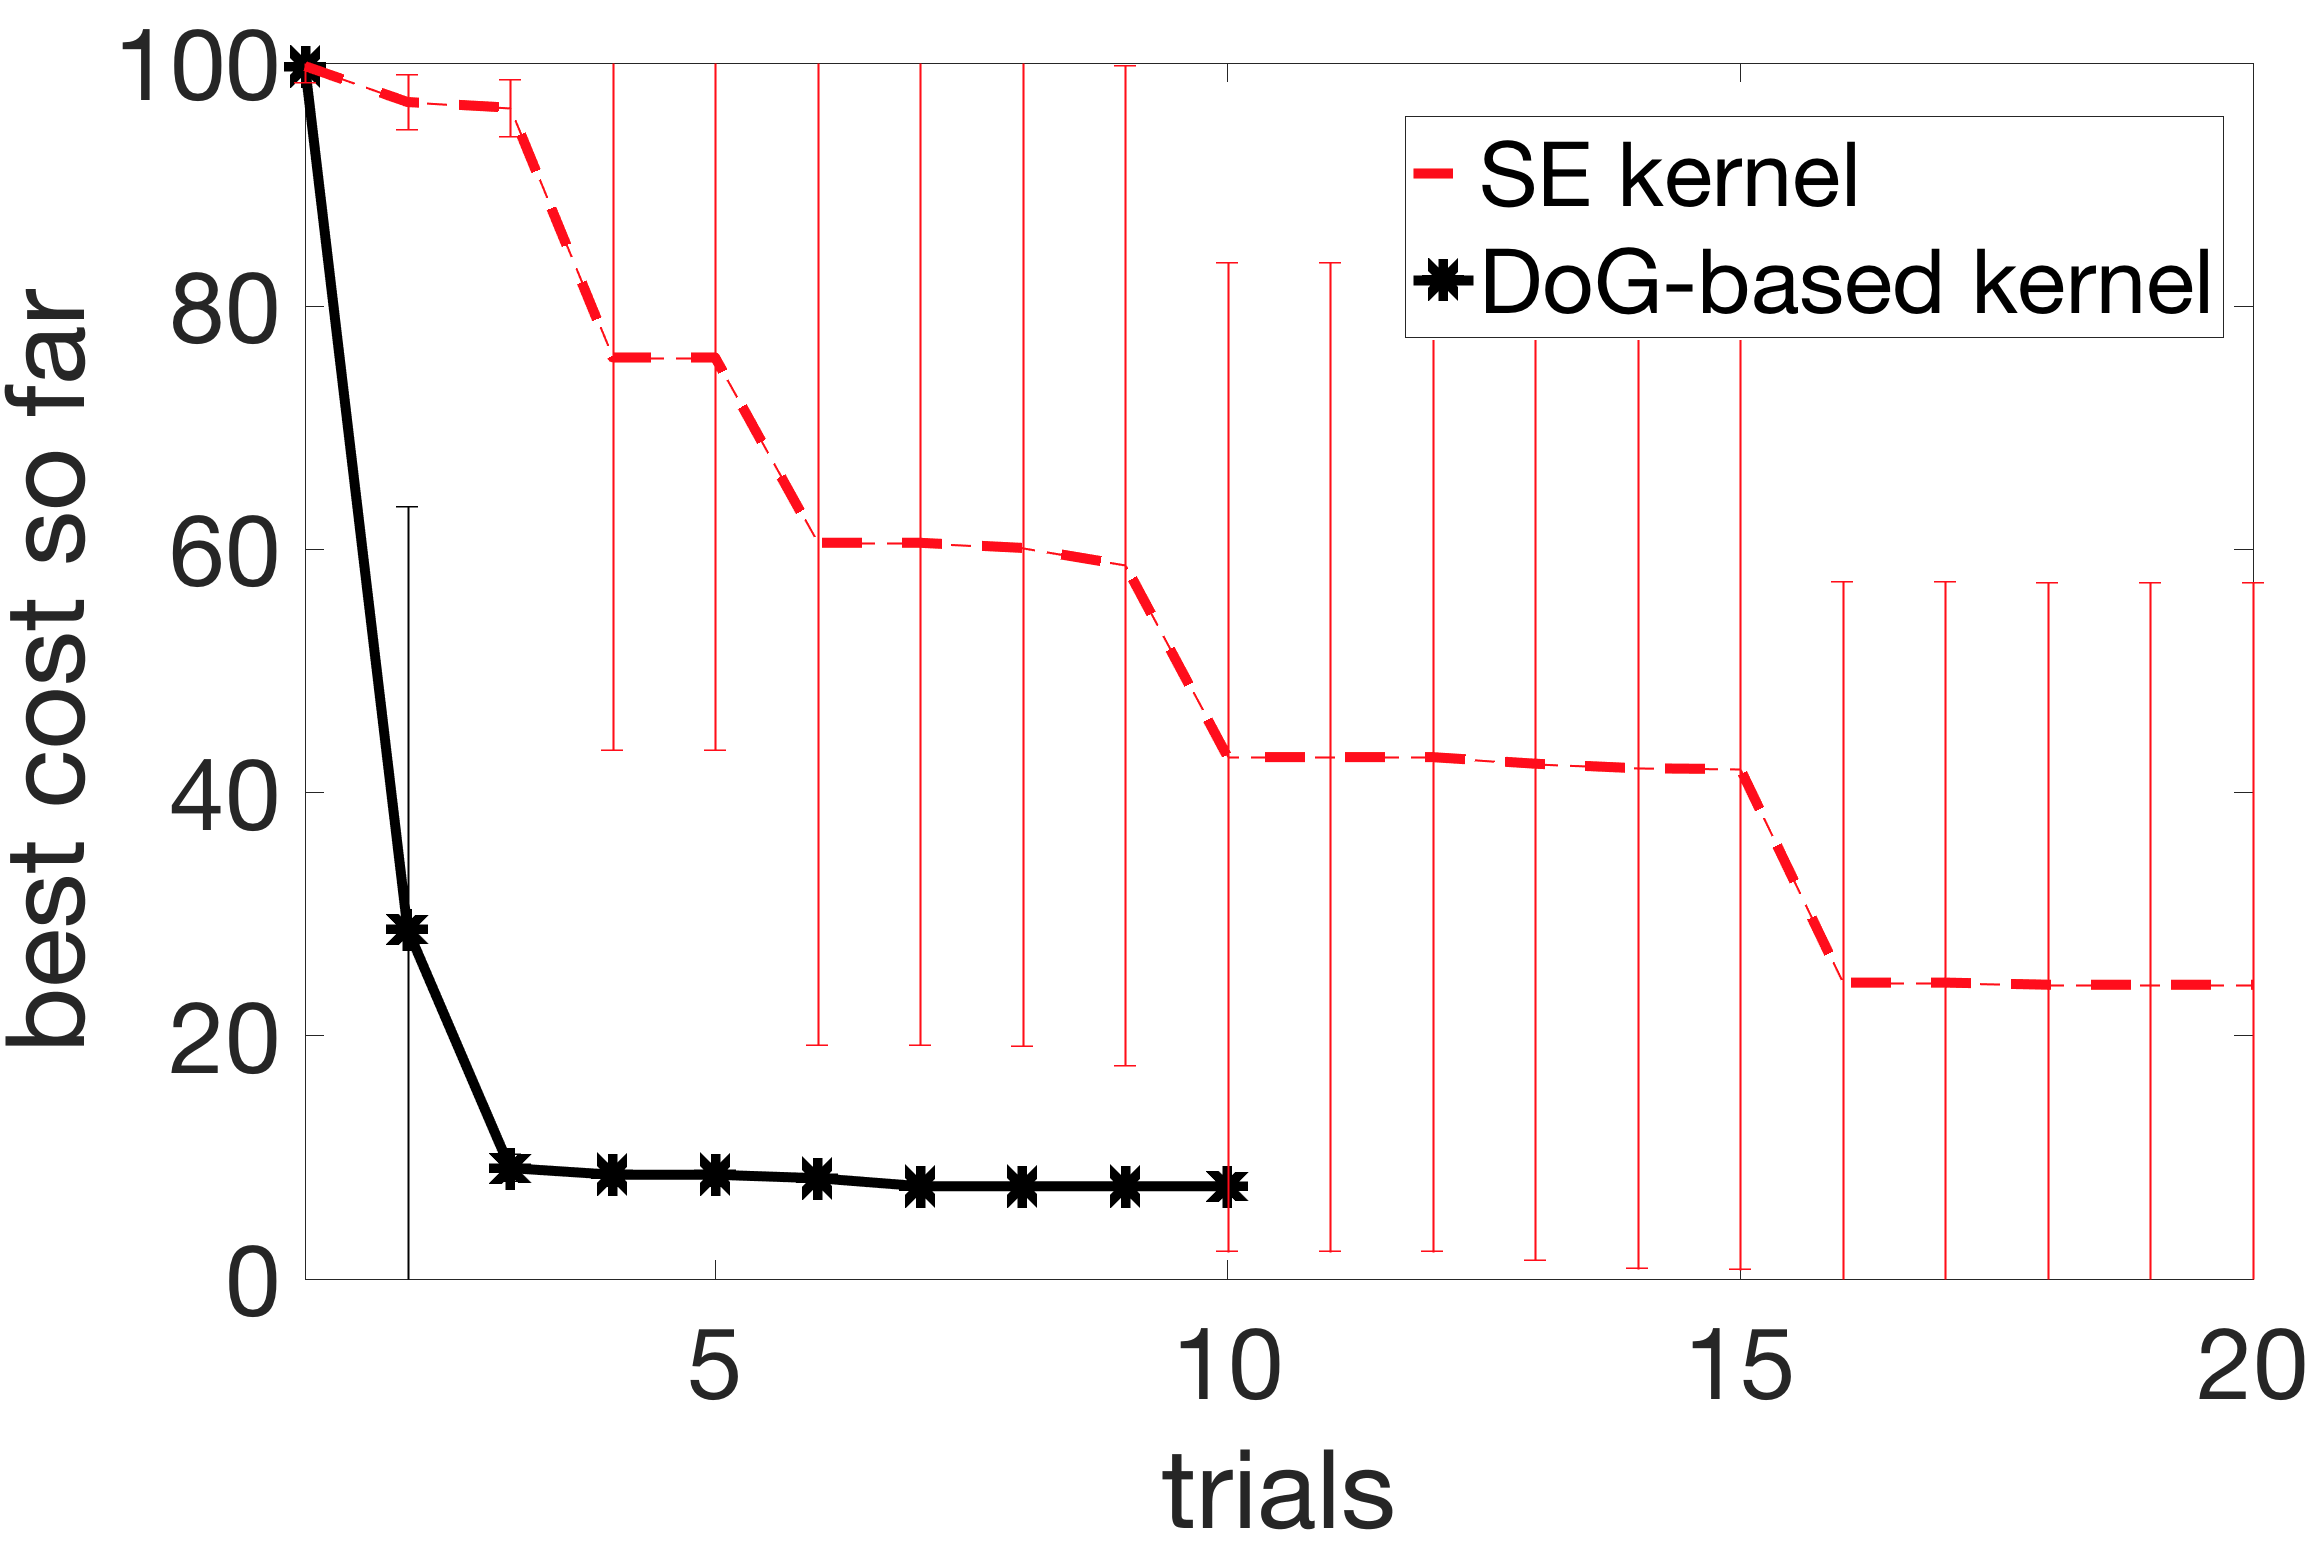
\includegraphics[width=0.6\textwidth]{img/hw_raibert_5d.png}
\caption{\small{BO for 5 dimensional controller on ATRIAS robot hardware. BO with SE finds walking points in 4/5 runs in 20 trials. BO with \dogkernel finds walking points in 5/5 runs in 3 trials.}}
\label{fig:hw_raibert_5d}
\end{figure}

On hardware, we conducted 5 runs of each -- BO with \dogkernel and BO with SE, 10 trials for \dogkernel per run, and 20 for SE kernel. In total, this led to 150 experiments on the robot (excluding the 100 random samples). We also experimented with using fixed vs automatically learned hyperparameters for both kernels. A simple choice of fixed hyperparameters worked well for \dogkernel, while for SE kernel it was better to learn these automatically. DoG scores were calculated on 20,000 points in simulation, by running $3.5s$ long simulations with target speed of $0.5m/s$.

BO with \dogkernel found walking points in 3 trials in 5/5 runs. BO with SE found walking points in 10 trials in 3/5 runs, and in 4/5 runs in 20 trials. These results can be seen in Figure \ref{fig:hw_raibert_5d}.

%\begin{figure}[b]
%\centering
%
\includegraphics[width=0.4\textwidth]{img/TODO.png}
%\caption{\small{Target speed profile and speed of the robot during a trial run on hardware. TODO: modify caption as needed}}
%\label{fig:bo_runs_atrias_hw_slides}
%\end{figure}

%-----------------------------------------------------
\subsection{Hardware experiments with the 9 dimensional controller}
\label{subsec:dog_9d}
The second set of hardware experiments were conducted on a 9-dimensional controller, described in Section \ref{sec:raibert_cont} on the ATRIAS robot. The target speed profile for these experiments was $0.4 m/s \text{ (30 steps)}$. The total number of steps before the controller shut off was $30$. The cost optimized was the same cost as in Equation \ref{eq:hdw_cost}. 

Again, we sampled 100 random points on hardware and 3 of them walked for this speed profile. This means that random sampling has a 1/33 chance of sampling a good point. On the variable speed profile from Section \ref{sec:hdw_5d}, the number of successful points out of 100 were 0, implying a less than 1\% success rate. To keep the problem at hand reasonable, we used the simpler target speed profile. In comparison, the success rate in simulation is 8\% for the tougher profile, implying a greater mismatch between hardware and simulation than the 5-dimensional controller. 

For this setting, we conducted 3 runs of each BO with \dogkernel and BO with SE, 10 trials for \dogkernel per run, and 10 for SE. In total, this led to 60 experiments on the hardware (excluding the random sampling). 

\begin{figure}[t]
\centering
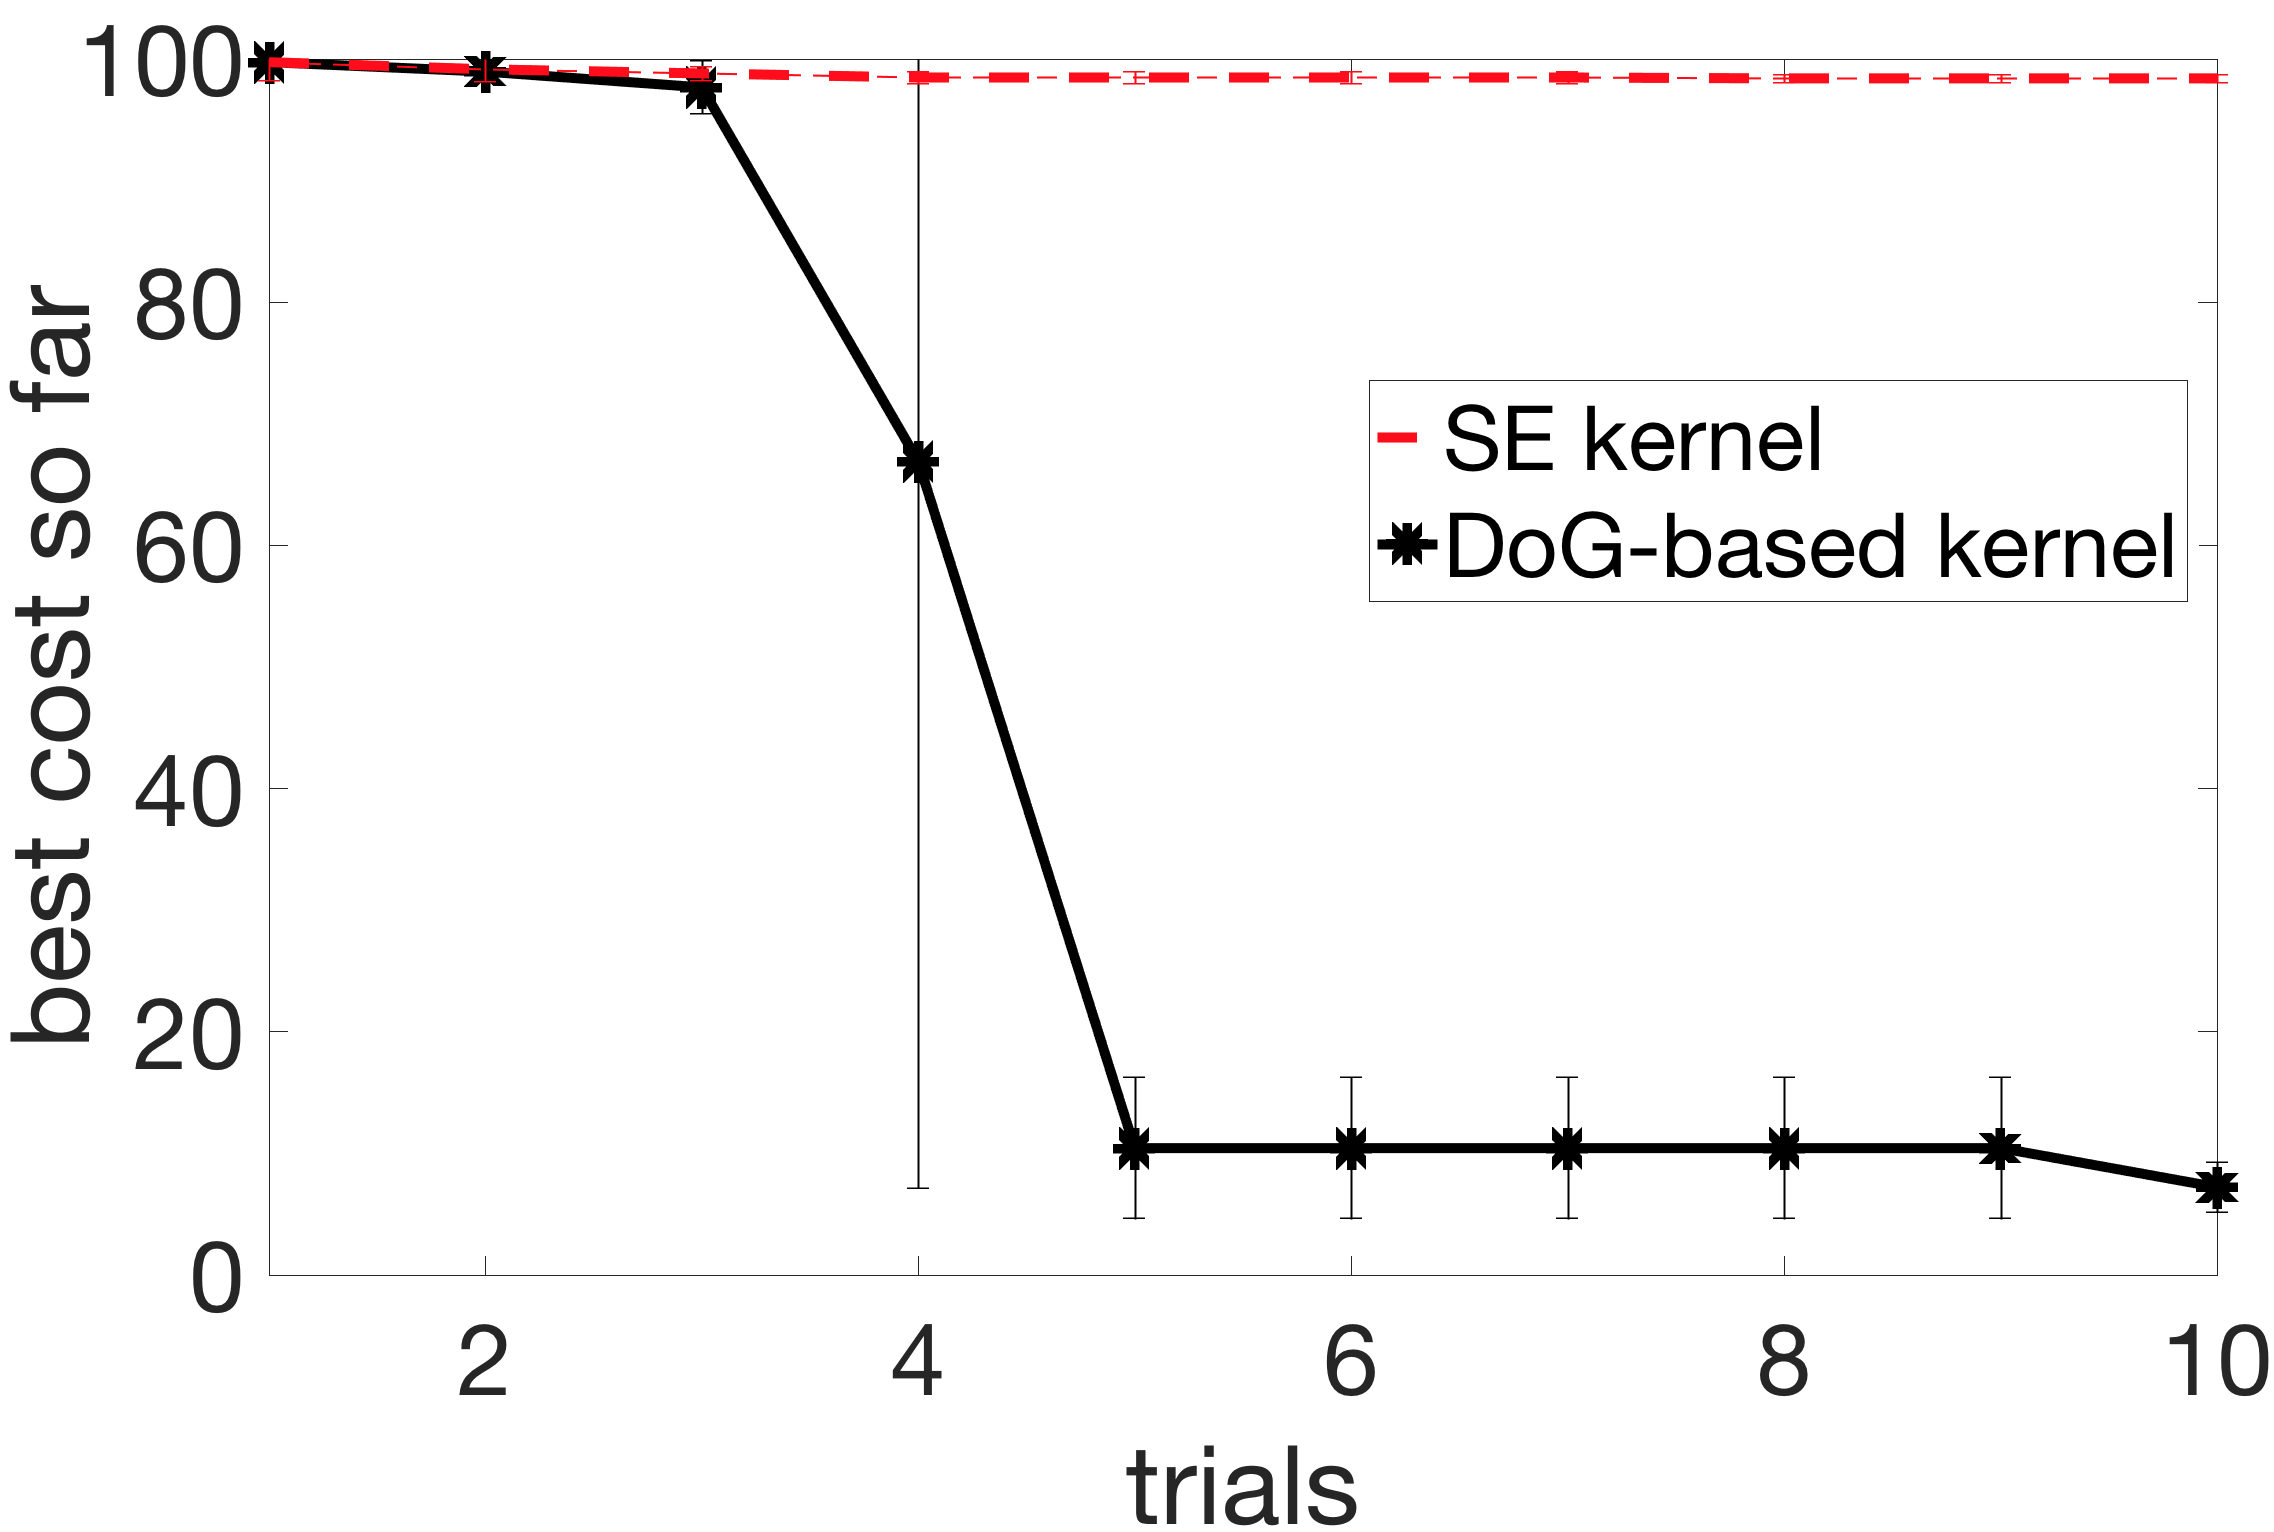
\includegraphics[width=0.6\textwidth]{img/hw_raibert_9d.png}
\caption{\small{BO for 9 dimensional controller on ATRIAS robot hardware. BO with SE doesn't sample any walking points in 3 runs. BO with \dogkernel finds walking points in 5 trials in 3/3 runs.}}
\label{fig:hw_raibert_9d}
\end{figure}

BO with \dogkernel found walking points in 5 trials in 3/3 runs. BO with SE did not find any walking points in 10 trials in all 3 runs. These results can be seen in Figure \ref{fig:hw_raibert_9d}.

Based on these results, we concluded that BO with \dogkernel was indeed able to extract useful information from simulation and speed up learning on hardware. However, it took slightly longer to find points for the 9-dimensional controller and the quality of solution might have improved further if we continued the optimization. This is all as per expectation, as a higher dimensional controller should take longer to optimize, but eventually lead to a better or as good a solution as a smaller dimensional controller. 

\begin{figure}
\centering
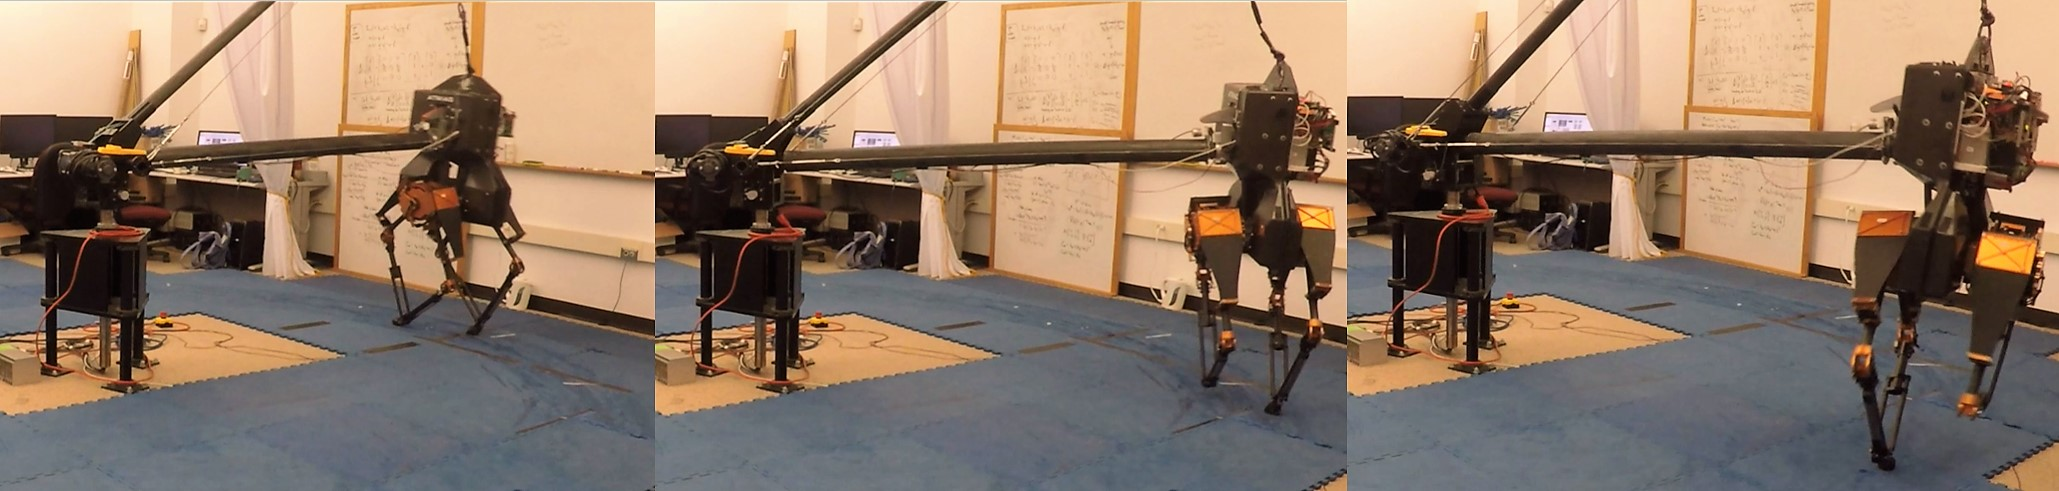
\includegraphics[width=0.98\textwidth]{img/atrias_time_lapse.jpg}
\caption{\small{A time lapse of ATRIAS walking around the boom during a run of \dogkernel.}}
\label{fig:bo_runs_atrias_hw_slides}
\end{figure}


\subsection{Simulation experiments with the 9-dimensional controller}

\label{sec:exps_sim}

To facilitate further experiments we used the ATRIAS simulator from ~\cite{martin2015robust} with modeling disturbances and a variable target speed profile of $0.4 m/s \text{ (15 steps)} - 0.6 m/s \text{ (15 steps)} - 1.0 m/s \text{ (15 steps)} - 0.6 m/s \text{ (15 steps)} - 0.2 m/s \text{ (5 steps)}$. For these experiments, we use the 9-dimensional controller described in \ref{sec:raibert_cont} as this proved to be a more challenging setting for the ATRIAS hardware. Masses of the robot torso, legs, the boom, as well as inertia of the torso were perturbed randomly by up to 15\% of their original values during optimization. This ensured a mismatch between the setting used to generate the kernel and the experimental setting for evaluating its performance, aimed at capturing the discrepancy between hardware and simulation. Note that the kernel was generated on the unperturbed setting, with parameters as described in Section \ref{sec:atrias} for a target speed of $0.5m/s$. The grid size for DoG scores was 100,000 points, and simulations were run for $5s$.

The cost used for these experiments was
\begin{equation}
\label{eq:cost_sim}
cost = 		
    \begin{cases}
		100 - x_{fall} , \text{\small{if fall}} \\
		||v_{avg} - v_{tgt}|| + c_{tr}, \text{\small{if walk}}\\
	\end{cases}
\end{equation}

where $x_{fall}$ is the distance covered before falling in meters, $v_{avg}$ is the average speed per step, $v_{tgt}$ is the target velocity for that step in $m/s$, and $c_{tr}$ captures the cost of transport - calculated by taking a sum of motor torques and normalizing them by a constant. Simulations for evaluating the cost were run for $30s$. Note the addition of the cost of transport in this cost, as compared to \ref{eq:hdw_cost}. $c_{tr}$ needs more than 10 trials to be optimized significantly, and the current low-level motor controllers in Section \ref{sec:raibert_cont} are not designed to reduce $c_{tr}$. Hence, its not considered in the hardware experiments.

\begin{figure}[t]
\centering
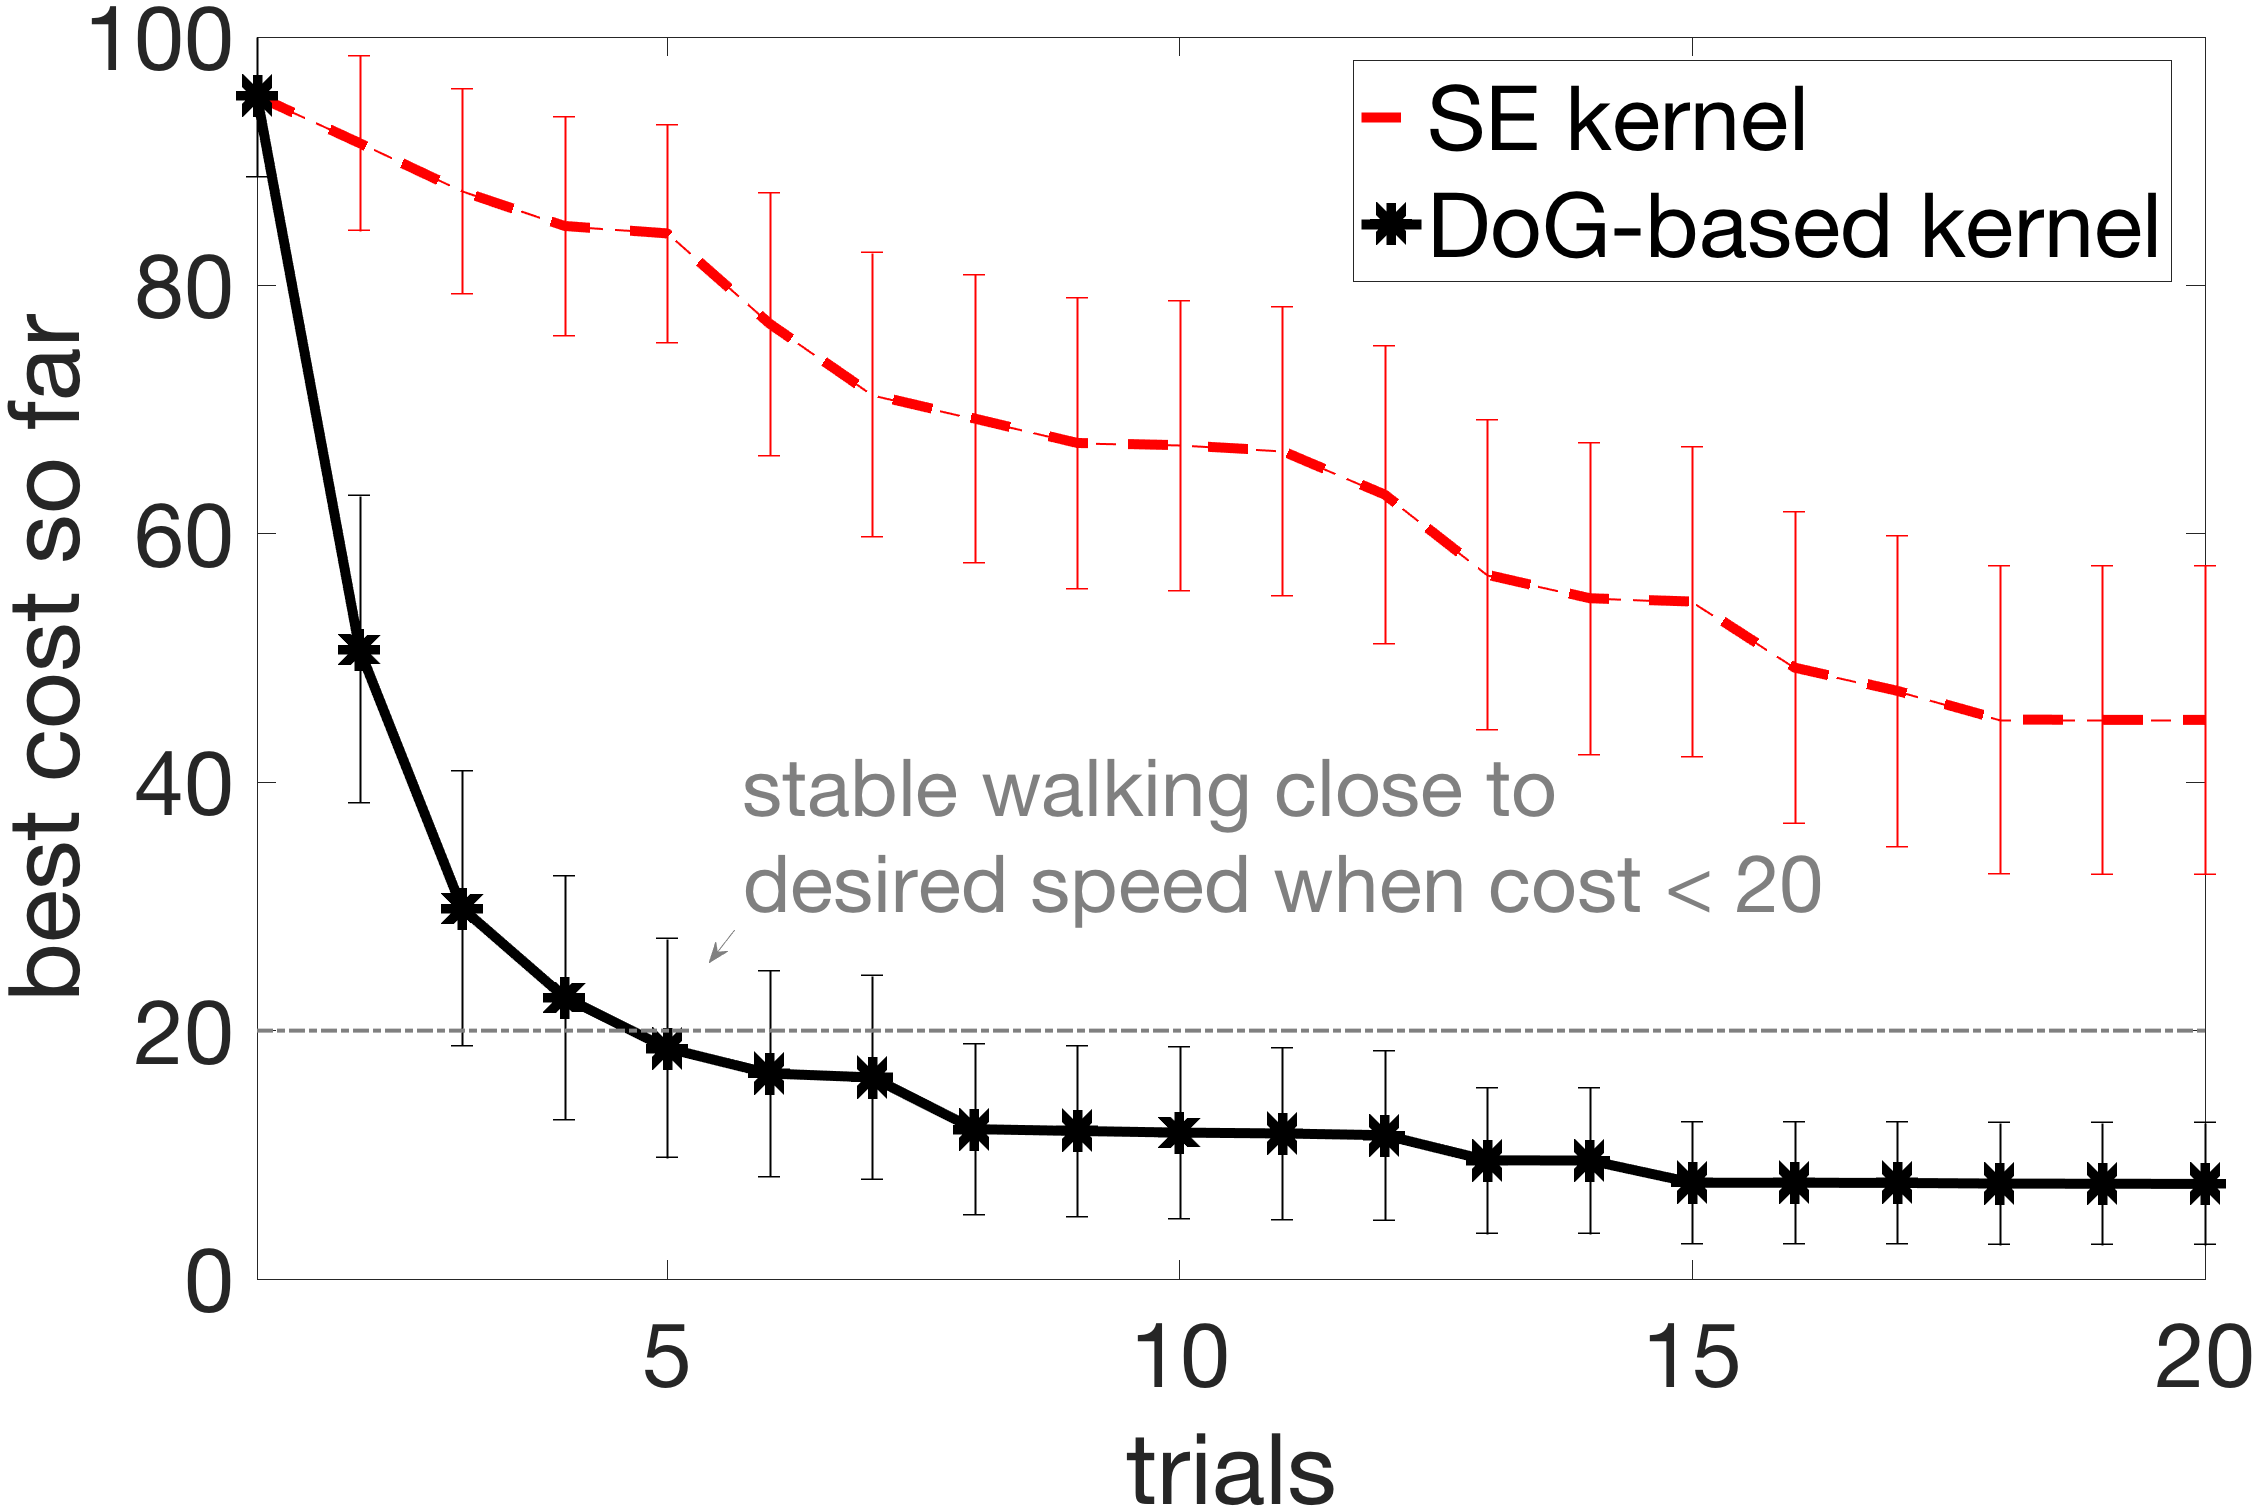
\includegraphics[width=0.6\textwidth]{img/sim_raibert_9d_speedupdown_disturbed_15.png}
\caption{\small{Further experiments using ATRIAS simulator: BO for ``speed-up-down'' target speed profile on robot model with mass and inertia differences
(mean over 50 runs; 95\% confidence intervals).}}
\label{fig:sim_9d_disturb}
\end{figure}

Figure~\ref{fig:sim_9d_disturb} illustrates BO on a simulated model with mass and inertia disturbances. The target was to start walking at 0.4m/s, then speed up to 0.6m/s, then 1.0m/s, slow down to 0.6m/s, then walk at 0.2m/s. \dogkernel was collected using an unperturbed model with a target speed of 0.5m/s, and yet it performed very well on this more challenging setting, with the top speed two times of the speed on which the kernel was collected. After 20 trials, 96\% of BO runs using the \dogkernel found a stable walking solution, compared to 56\% of the runs using an SE kernel. The average cost of the walking solutions was also improved: lower by $\approx$30\% when using DoG vs SE kernel.

These experiments suggest that \dogkernel is able to offer improvement for the settings different from the one used to generate it. This improvement is robust to both the deviations of the robot model/hardware parameters as well as desired walking speed profiles.

\subsection{Simulation experiments with the 50-dimensional controller}

\label{sec:vnmc_expt}
Next set of experiments were using the VNMC 50-dimensional controller, as described in Section \ref{sec:VNMC_cont} on the ATRIAS simulation.

VNMC does not start from rest, and needs an initial velocity. In previous work this has been emulated by either giving simulations initial speeds, or by giving a push. These are either un-realizable or unreliable on hardware. To overcome this problem, we start the VNMC with a \mbox{5-dimensional} walking controller (described in Section \ref{sec:raibert_cont}, parameters hand-tuned and fixed). Once the robot has taken 10 steps with this controller, the control is switched to VNMC. 

To construct \dogkernel for this controller we collected 250,000 points from 7-second simulations. The DoG scores were computed after switching to the VNMC (so after first 10 steps). Searching in 50 dimensional space could be completely intractable if the search region is too large. Usually enough domain knowledge is available to confine the search to a reasonably manageable region. We tried to hand-tune an initial point that walked 3-4 steps before falling in simulation (this point still had a very high cost of $\approx\!\!93$). This point became the ``center" of our search space, and we searched in a hyper-cube of size $[0.75, 1.25]$ in each dimension around this point. So, with initial point $x_0$, the search space was $[0.75 \cdot x_0 , 1.25 \cdot x_0]$. With these boundaries, 4\% of points sampled randomly in simulation were walking.

\begin{figure}[t]
\centering
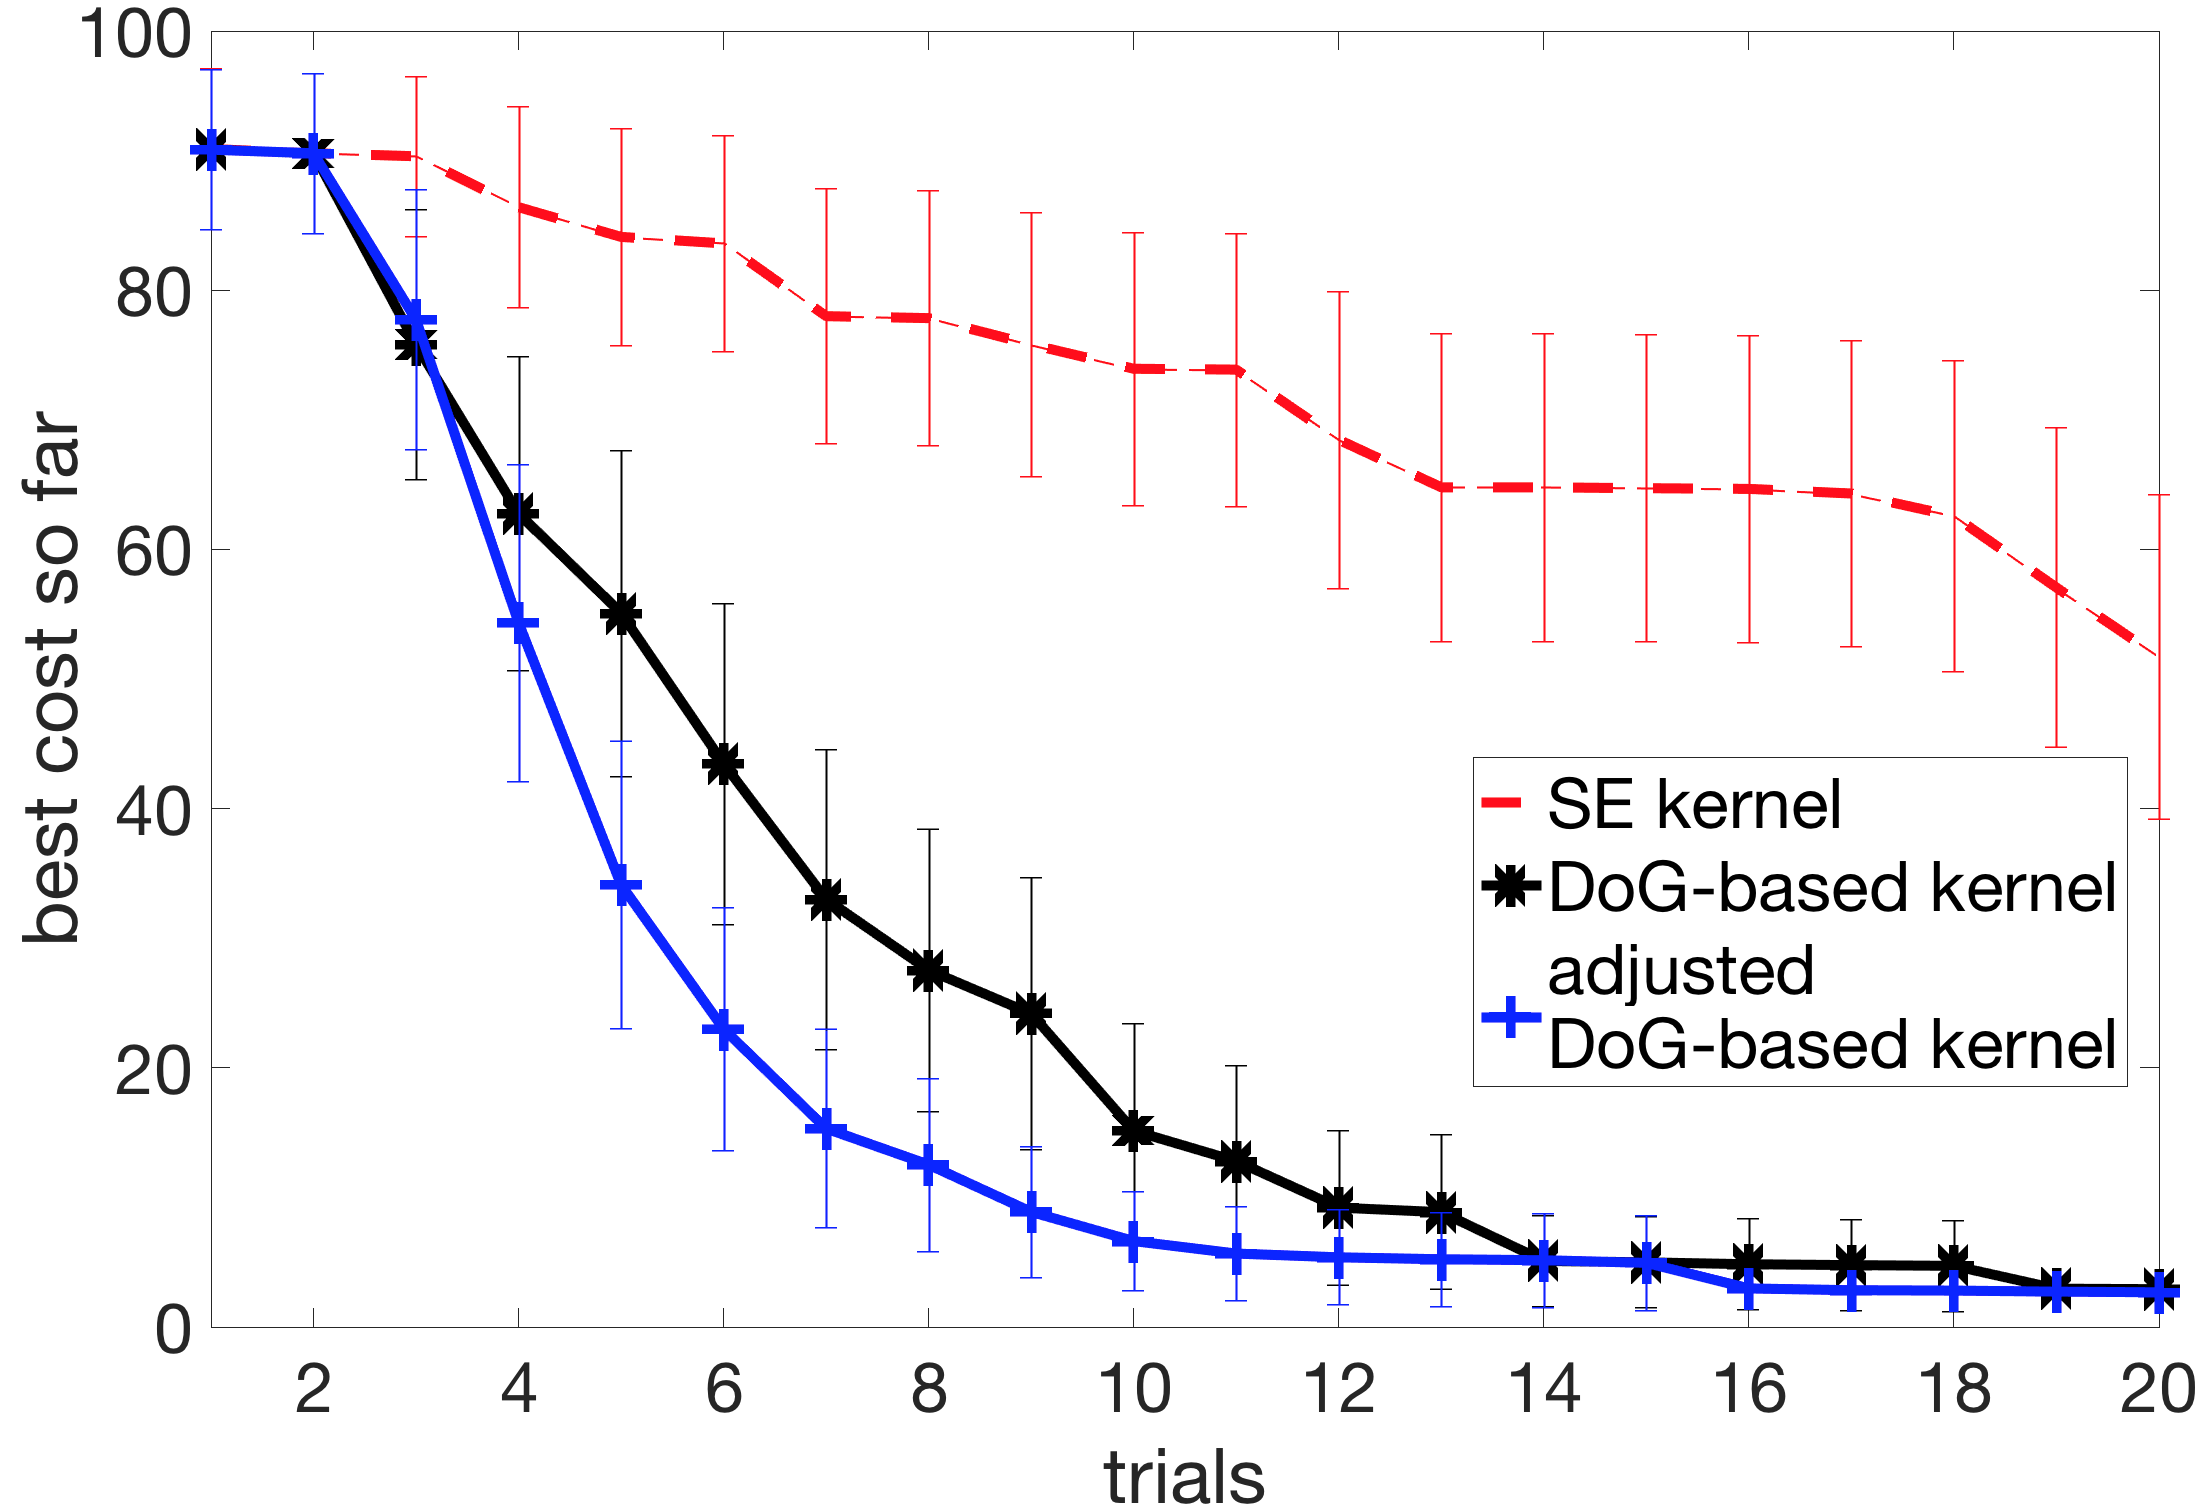
\includegraphics[width=0.6\textwidth]{img/sim_NM_Atrias_50d.png}
\caption{\small{BO with 50-dimensional Virtual Neuromuscular Controller on the ATRIAS simulation.}}
\label{fig:sim_NM_Atrias_50d}
\end{figure}

Figure \ref{fig:sim_NM_Atrias_50d} shows results of Bayesian Optimization with SE, \dogkernel and adjusted \dogkernel with mismatch information. During optimization simulations were run for $30$ seconds. We used the same cost function as described in the previous section (equation~\ref{eq:cost_sim}).

In 50-dimensional control, the mismatch between long and short simulations becomes apparent. This raises concerns for how useful \dogkernel would be on hardware, since it tries to infer the quality of the controller parameters from short simulations. 
For the 5-dimensional and 9-dimensional controllers, the performance during short simulations usually predicted whether $30s$ simulations would be successful. That is, points that walk for 5s would usually walk for 30s. However, this is not true for the 50-dimensional controller. Since this controller is capable of much richer behaviors, if a point is not in a limit cycle before the end of a short simulation, it can lead to a range of behaviours later. As a result, we noticed an improvement when using adjusted \dogkernel described in Section~\ref{sec:mismatch}. While DoG is still very competitive and finds walking points in 100\% of the runs by 20 trials, the adjusted DoG with mismatch has an advantage. It reaches the same performance as \dogkernel, but faster. 

%The 50-dimensional controller has not been fully implemented to work on hardware yet due to lack of time. However, our experiments on other controllers so far seem promising and we are working towards a hardware implementation. 
%\RA{describe current progress and interest in this controller being ultimately used on hw ~\ref{van2015experimental}}
To anticipate potential mismatch between simulation and hardware, we tested it on slightly perturbed initial conditions for the VNMC. The different conditions were aimed to replicate issues likely to be seen on hardware. The starting states for VNMC would differ slightly each time, since they would depend on the state of the robot after the 5-dimensional initiating controller has finished. Both DoG and adjusted DoG were robust to slight changes in initial condition. 

It would be interesting to study the effect of a mismatch map on performance on hardware. While essentially a mismatch map adds more parameters to learn, which would result in a slower optimization, if initialized properly with domain knowledge, it might help. The \dogkernel samples a few unstable points in the start of the 50-dimensional optimization, as these have high DoG scores on short simulations, but still might fall in longer simulations under disturbances. Since a lot of the 50-dimensional space is clustered around each DoG score, its an over-condensation of the space. A lot of potentially good points get rejected because one of the points falls. If we detect a mismatch at the high DoG point that fell, and effectively increase its distance to other high DoG points, we will help speed up the optimization.

%We plan to test adjusted \dogkernel more in the future in this challenging setting that could be sensitive to simulation-hardware mismatch. 

\subsection{Simulation experiments on a 16-dimensional controller}
\label{sec:7_link_expts}
To make sure that our feature transform generalizes to multiple robot morphologies, we also did experiments on the 7-link biped, described in Section \ref{sec:7_link_biped}.

\begin{figure}[t]
\centering
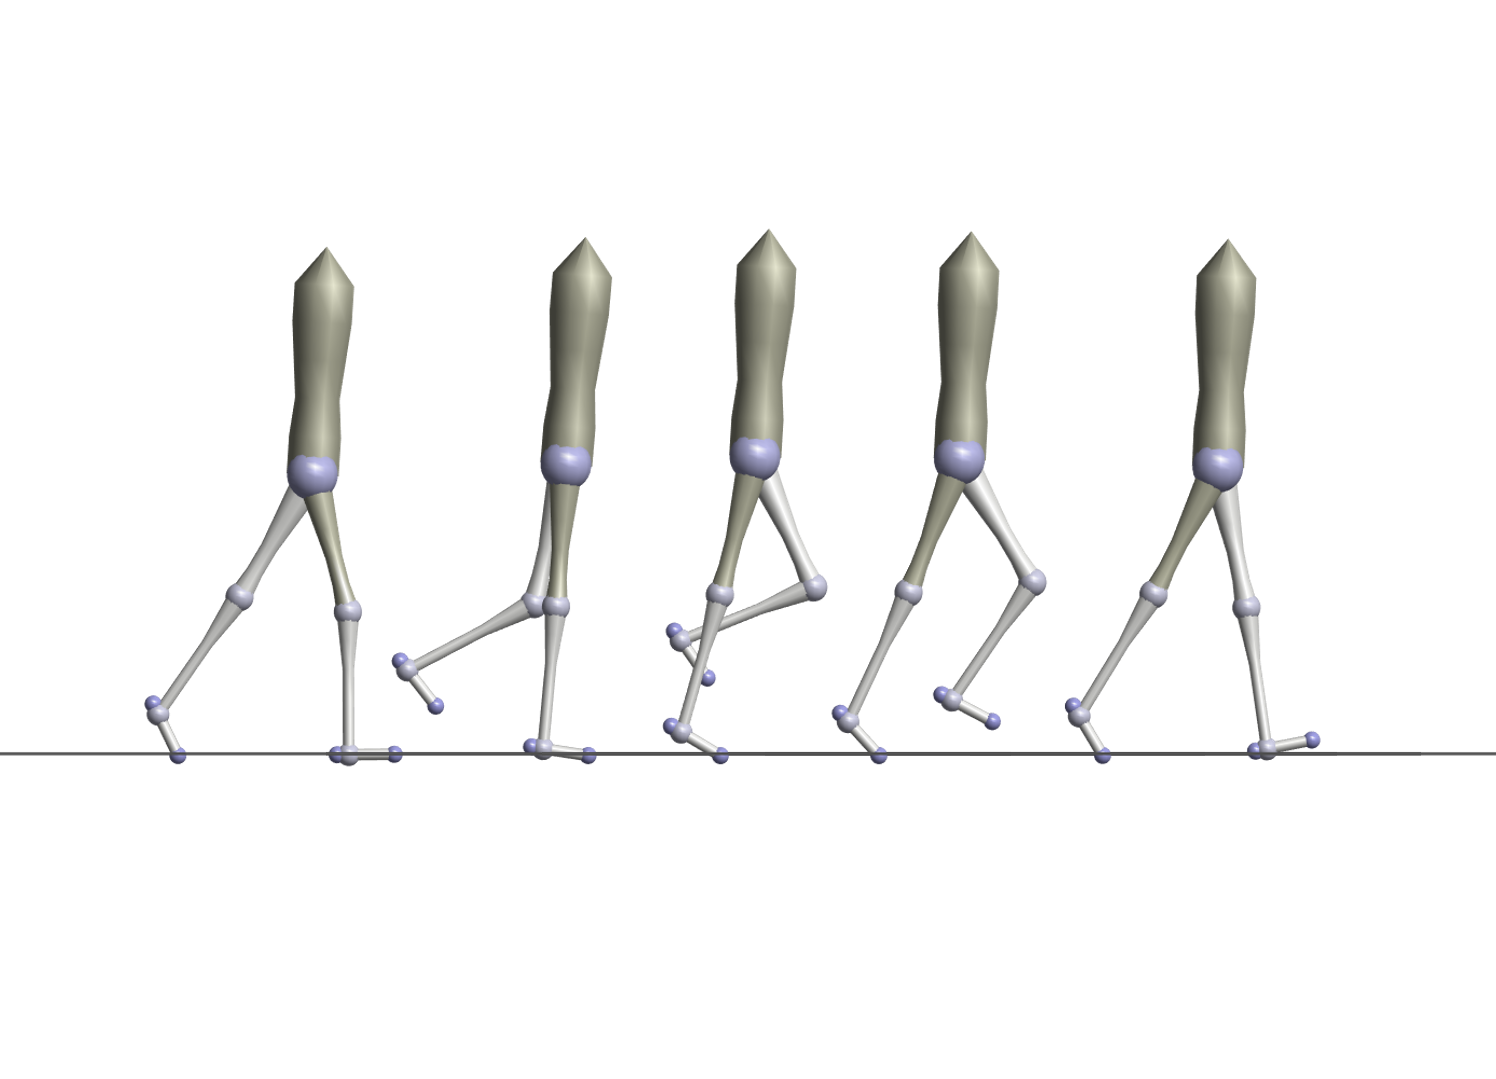
\includegraphics[width=0.35\textwidth]{img/walk_flat.png}
\hspace{10px}
\vspace{-40px}
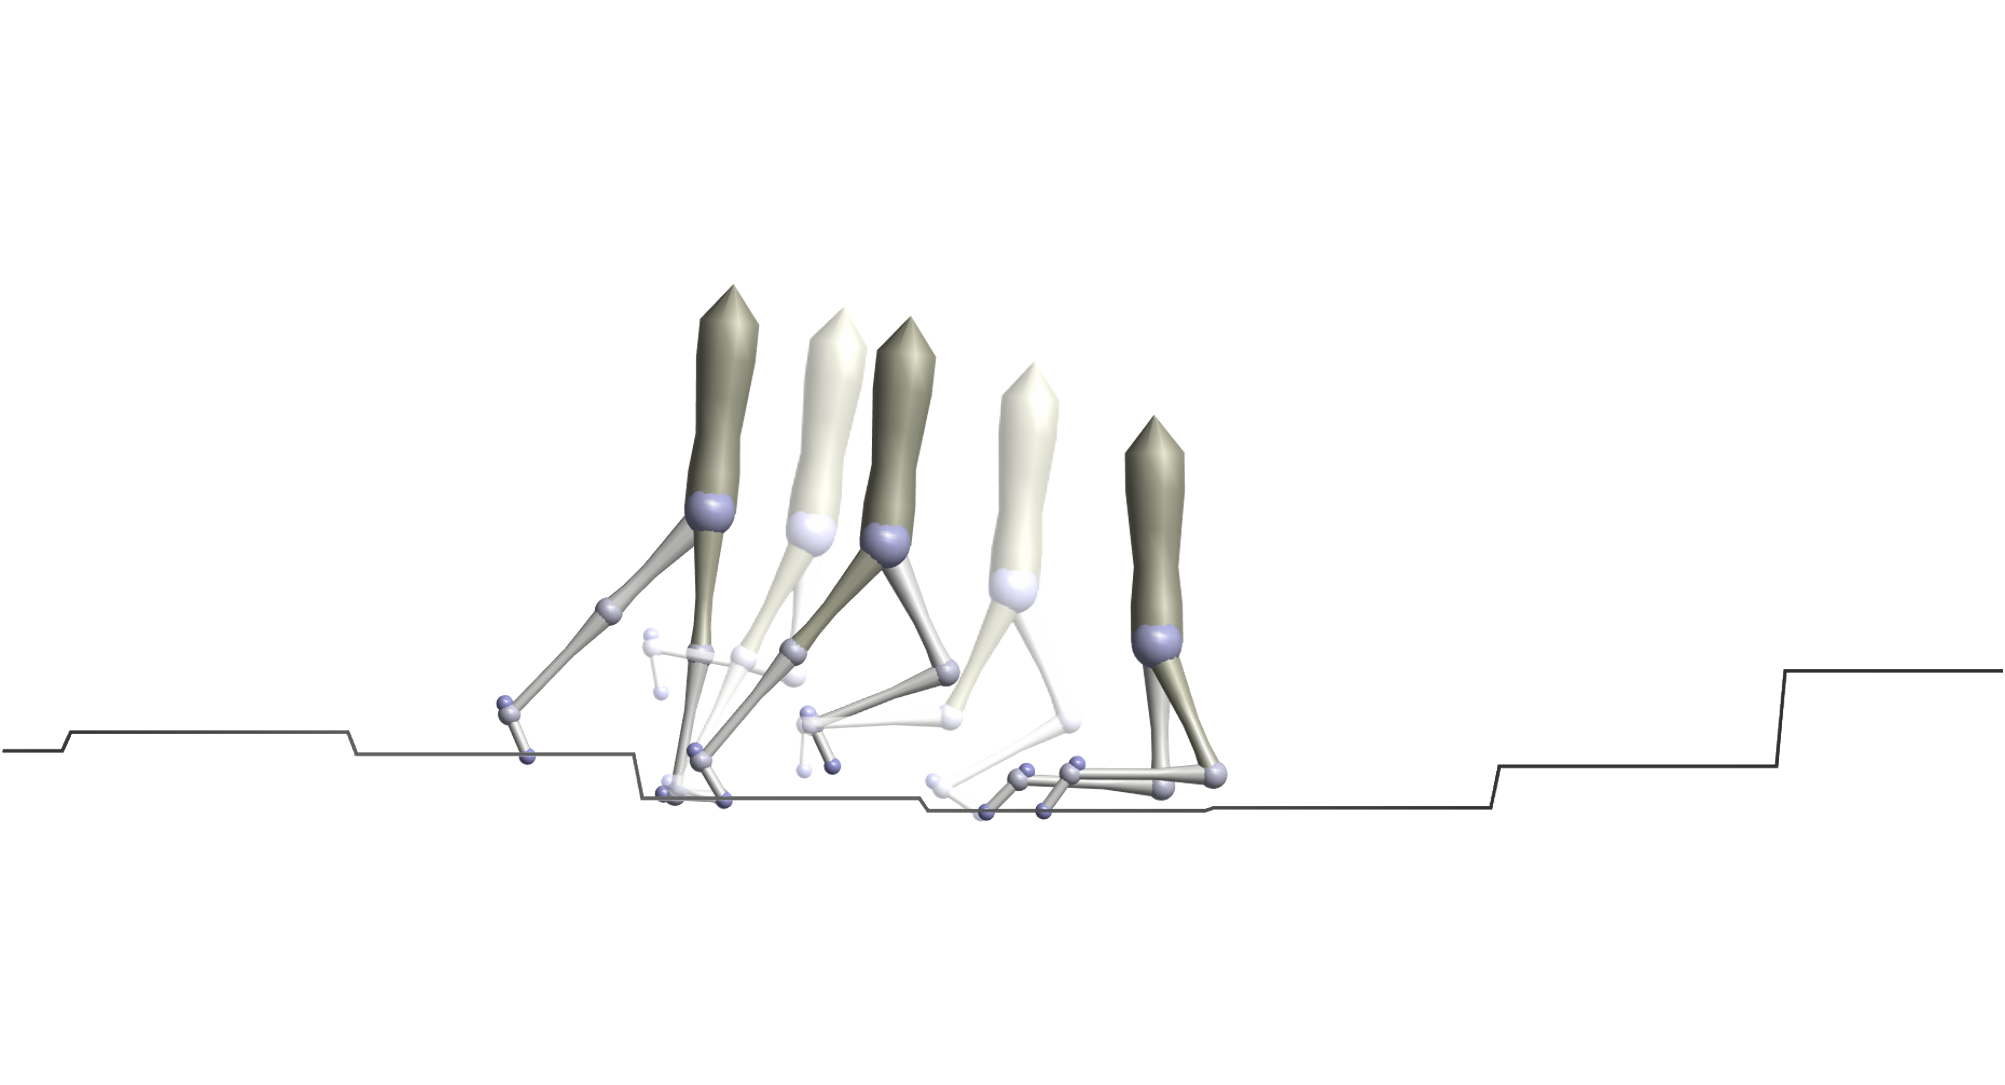
\includegraphics[width=0.5\textwidth]{img/rough_fall.png}
\label{fig_bo_locomotion_visualization_rough}
\vspace{30px}
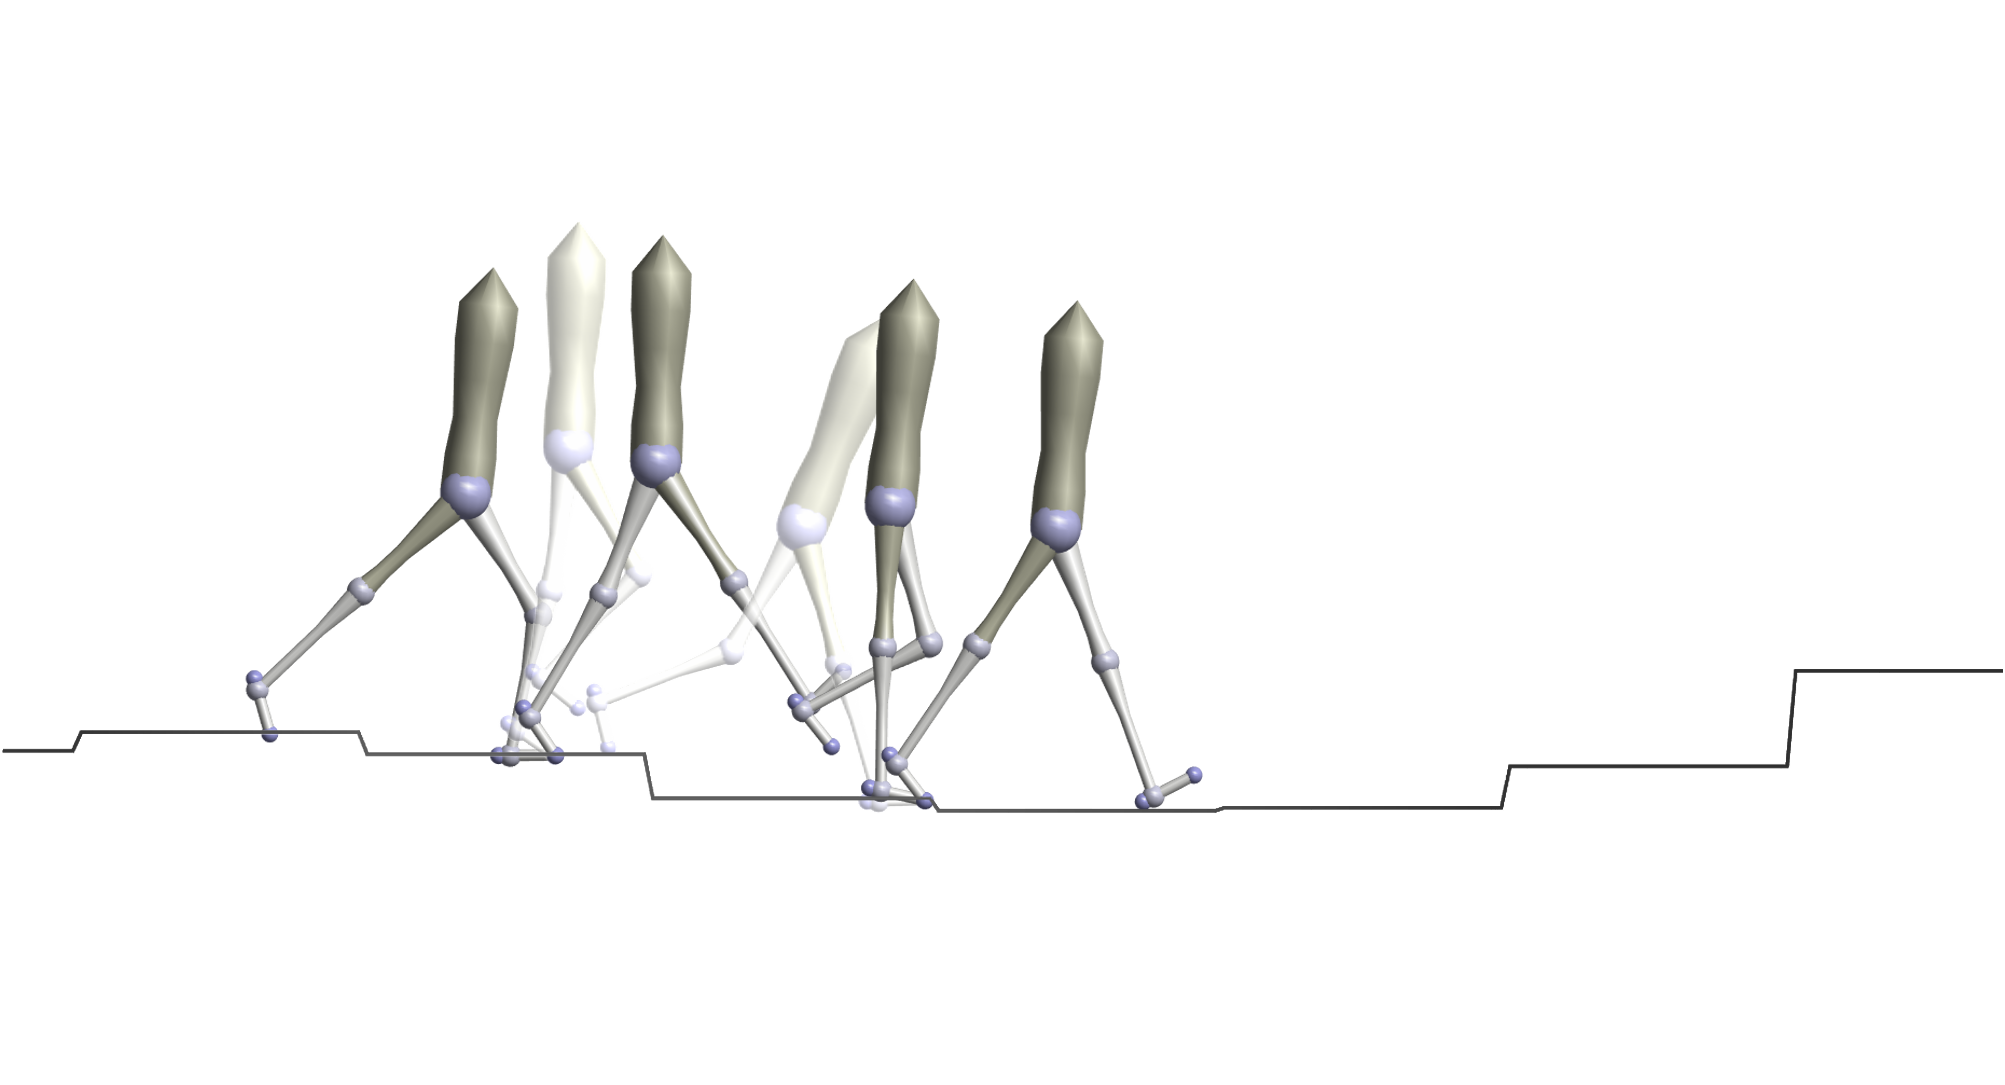
\includegraphics[width=0.5\textwidth]{img/rough_walk.png}
\caption{Top row: a policy that generates successful walking on flat ground could fail on rough ground. Bottom row: optimization on rough ground finds policies that walk, even though pre-computation for DoG kernel is done using unperturbed model on flat ground.}
\label{fig_bo_locomotion_visualization_flat}
\end{figure}

We conduct our experiments on models with mass and inertial disturbances and on different ground profiles. After collecting the DoG scores, we perturb the mass of each link, inertia and center of mass location randomly by up to $15\%$ of the original value. For mass/inertia we randomly pick a variable from a uniform distribution between $[-0.15,\ 0.15] \cdot M$, where $M$ is the original mass/inertia of the segment. Similarly we change the location of the center of mass by $[-0.15,\ 0.15] \cdot L/2$, where $L$ is the length of the link. These disturbances are different for each run of our algorithm, hence we test a wide range of possible modelling disturbances.
For the ground profiles, we generate random ground height disturbances of upto $\pm 8cm$ per step. This is a significant disturbance that can make successful controllers on flat ground fall, as shown in Figure \ref{fig_bo_locomotion_visualization_flat}.

To ensure that our approach can perform well across various cost functions, we conduct experiments on two different costs, constructed such that parameter sets achieving low cost also achieve stable and robust walking gaits. The first cost function varies smoothly over the parameter space:
 
\begin{align}
cost = \frac{1}{1+t} + \frac{0.3}{1+d} + 0.01 (v-v_{tgt}),
\end{align}
where $t$ is seconds walked, $d$ is the final CoM position, $v$ is mean velocity and $v_{tgt}$ is the desired walking velocity (from human data). This cost encourages walking further and for longer through the first two terms, and penalizes deviating from the target velocity with the last.

The second cost function is a slightly modified version of the cost used in~\cite{song2015neural} for experiments with \mbox{CMA-ES}, also similar to the cost described in previous sections. It penalizes policies that lead to falls in a non-smooth manner:
\begin{align}
cost_{non-smooth} = 		
    \begin{cases}
		300 - x_{fall} , \text{\small{if fall}} \\
		100 ||v_{avg} - v_{tgt}|| + c_{tr}, \text{\small{if walk}}\\
	\end{cases}
\end{align}
Here $x_{fall}$ is the distance travelled before falling, $v_{avg}$ is the average speed in simulation, $v_{tgt}$ is the target speed and $c_{tr}$ is the cost of transport calculated using muscle activations. The first term directly penalizes policies that result in a fall, inversely to the distance walked. If the model walks for the whole simulation time, the cost is lower, ensured by the constants, and encourages policies that result in lower cost of transport and walk at target velocity. Since we have the same set of gains for left and right legs, the steadiness cost of the original cost~\cite{song2015neural} was unimportant. So, we removed that term and focused on the first and second conditions in the optimization.

In the following sections we compare the performance of several baseline and state-of-the-art optimization algorithms in simulation. Motivated by the discussion in~\cite{calandra2016bayesian}, we include the baseline of uniform random search. While this search is uninformed and not sample-efficient, it could (perhaps surprisingly) serve as a competitive baseline in non-convex high-dimensional optimization problems. 
%Theoretically -- it provides statistical guarantees of convergence, and practically -- it can outperform informed algorithms as well as grid search on high-dimensional problems (see Section~2~in~\cite{calandra2016bayesian} for further discussion).

We also provide comparisons with \mbox{CMA-ES}~\citep{hansen2006cma} and Bayesian Optimization with a Squared Exponential kernel (basic BO). Since we were optimizing a non-convex function in a 16D space, it was not feasible to calculate the global minimum exactly. To estimate the global minimum for the costs we used, we ran CMA-ES (until convergence) and BO with our domain kernel (for 100 trials) for 50 runs without model disturbances on flat ground. 
When reporting results, we plot the best results found in this easier setting as the estimated optimum for comparison.

All the experiments described below are done for 50 independent runs, each with a unique set of modeling disturbances and a different ground profile for rough ground walking. Each run  consists of 100 trials or cost function evaluations, in which the optimization algorithm evaluates a parameter set for 100 seconds of simulation. Note that the disturbances and ground profiles remain constant across each run (100 trials).

\subsubsection{Experiments on the smooth cost function}

\begin{figure}[t]
\centering
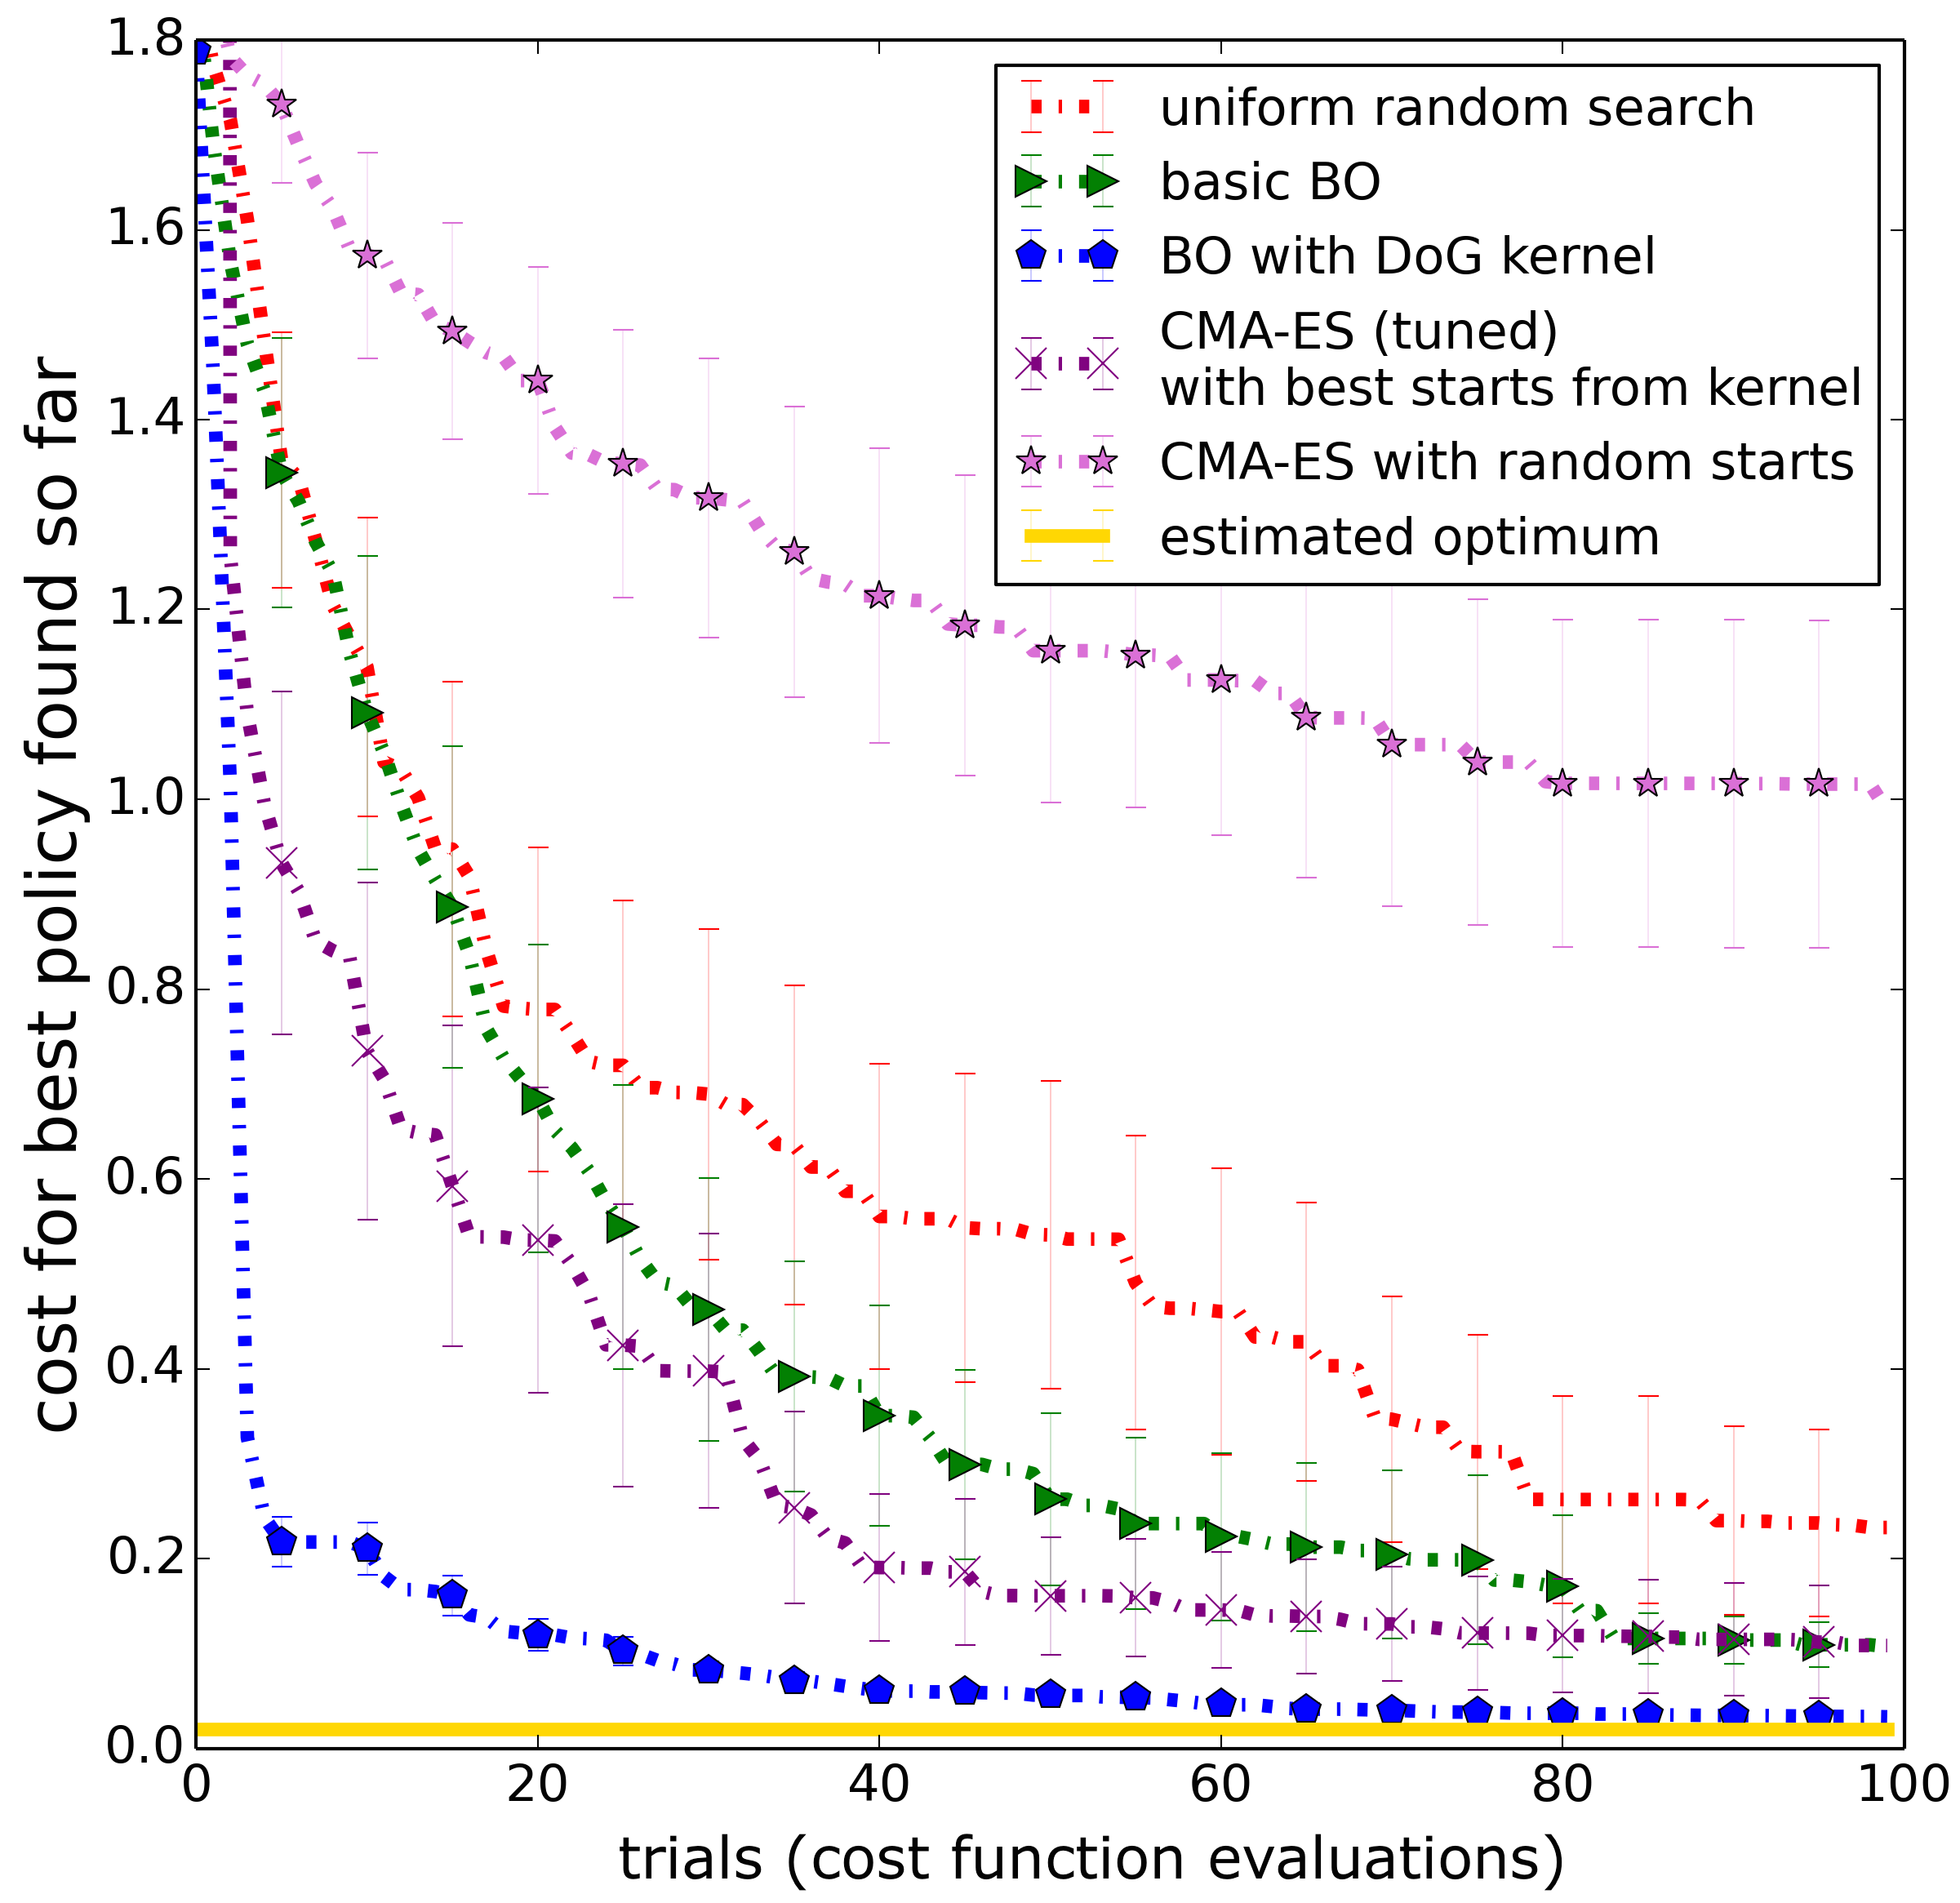
\includegraphics[width=0.6\textwidth]{img/rnd_bo_bo_covLoc_cma_rough6_disturb_smooth_cost.png}
\caption{Experiments using DoG kernel on rough ground with model disturbances on the smooth cost over 50 runs. Basic BO line (green triangles) was obtained using BO with a Euclidean distance kernel. Estimated optimum (yellow line) was obtained on the unperturbed setting. BO with \dogkernel kernel (blue pentagons) used the DoG feature transform and was substantially more sample-efficient than the alternative approaches.}
\label{fig_bo_locomotion}
\end{figure}

Figure~\ref{fig_bo_locomotion} shows results of our experiments using the \dogkernel kernel on the smooth cost.
Policies with costs of less than $\approx\!\!0.15$ corresponded to robot model walking on rough ground with $\pm 8 cm$ disturbance.
For BO with \dogkernel kernel, 25-30 cost function evaluations were sufficient to find points that corresponded to robot model walking on a randomly generated rough ground. This is in contrast to basic BO that did not find such results in under 100 trials. 

To let CMA-ES also benefit from the kernel, we started each run from one of the best 100 points for the \dogkernel kernel. After tuning the $\sigma$ parameter of CMA-ES to make it exploit more around the starting point, we were able to find policies that resulted in walking on rough ground after 65-70 cost function evaluations on most runs. On the other hand, \mbox{CMA-ES} starting from a random initial point was not able to find walking policies in 100 evaluations.

These results suggest that DoG scores successfully captured useful information about the parameter space and were able to effectively focus BO and CMA-ES on the promising regions of the policy search space. 

\subsubsection{Experiments with the non-smooth cost}

\begin{figure}[t]
\centering
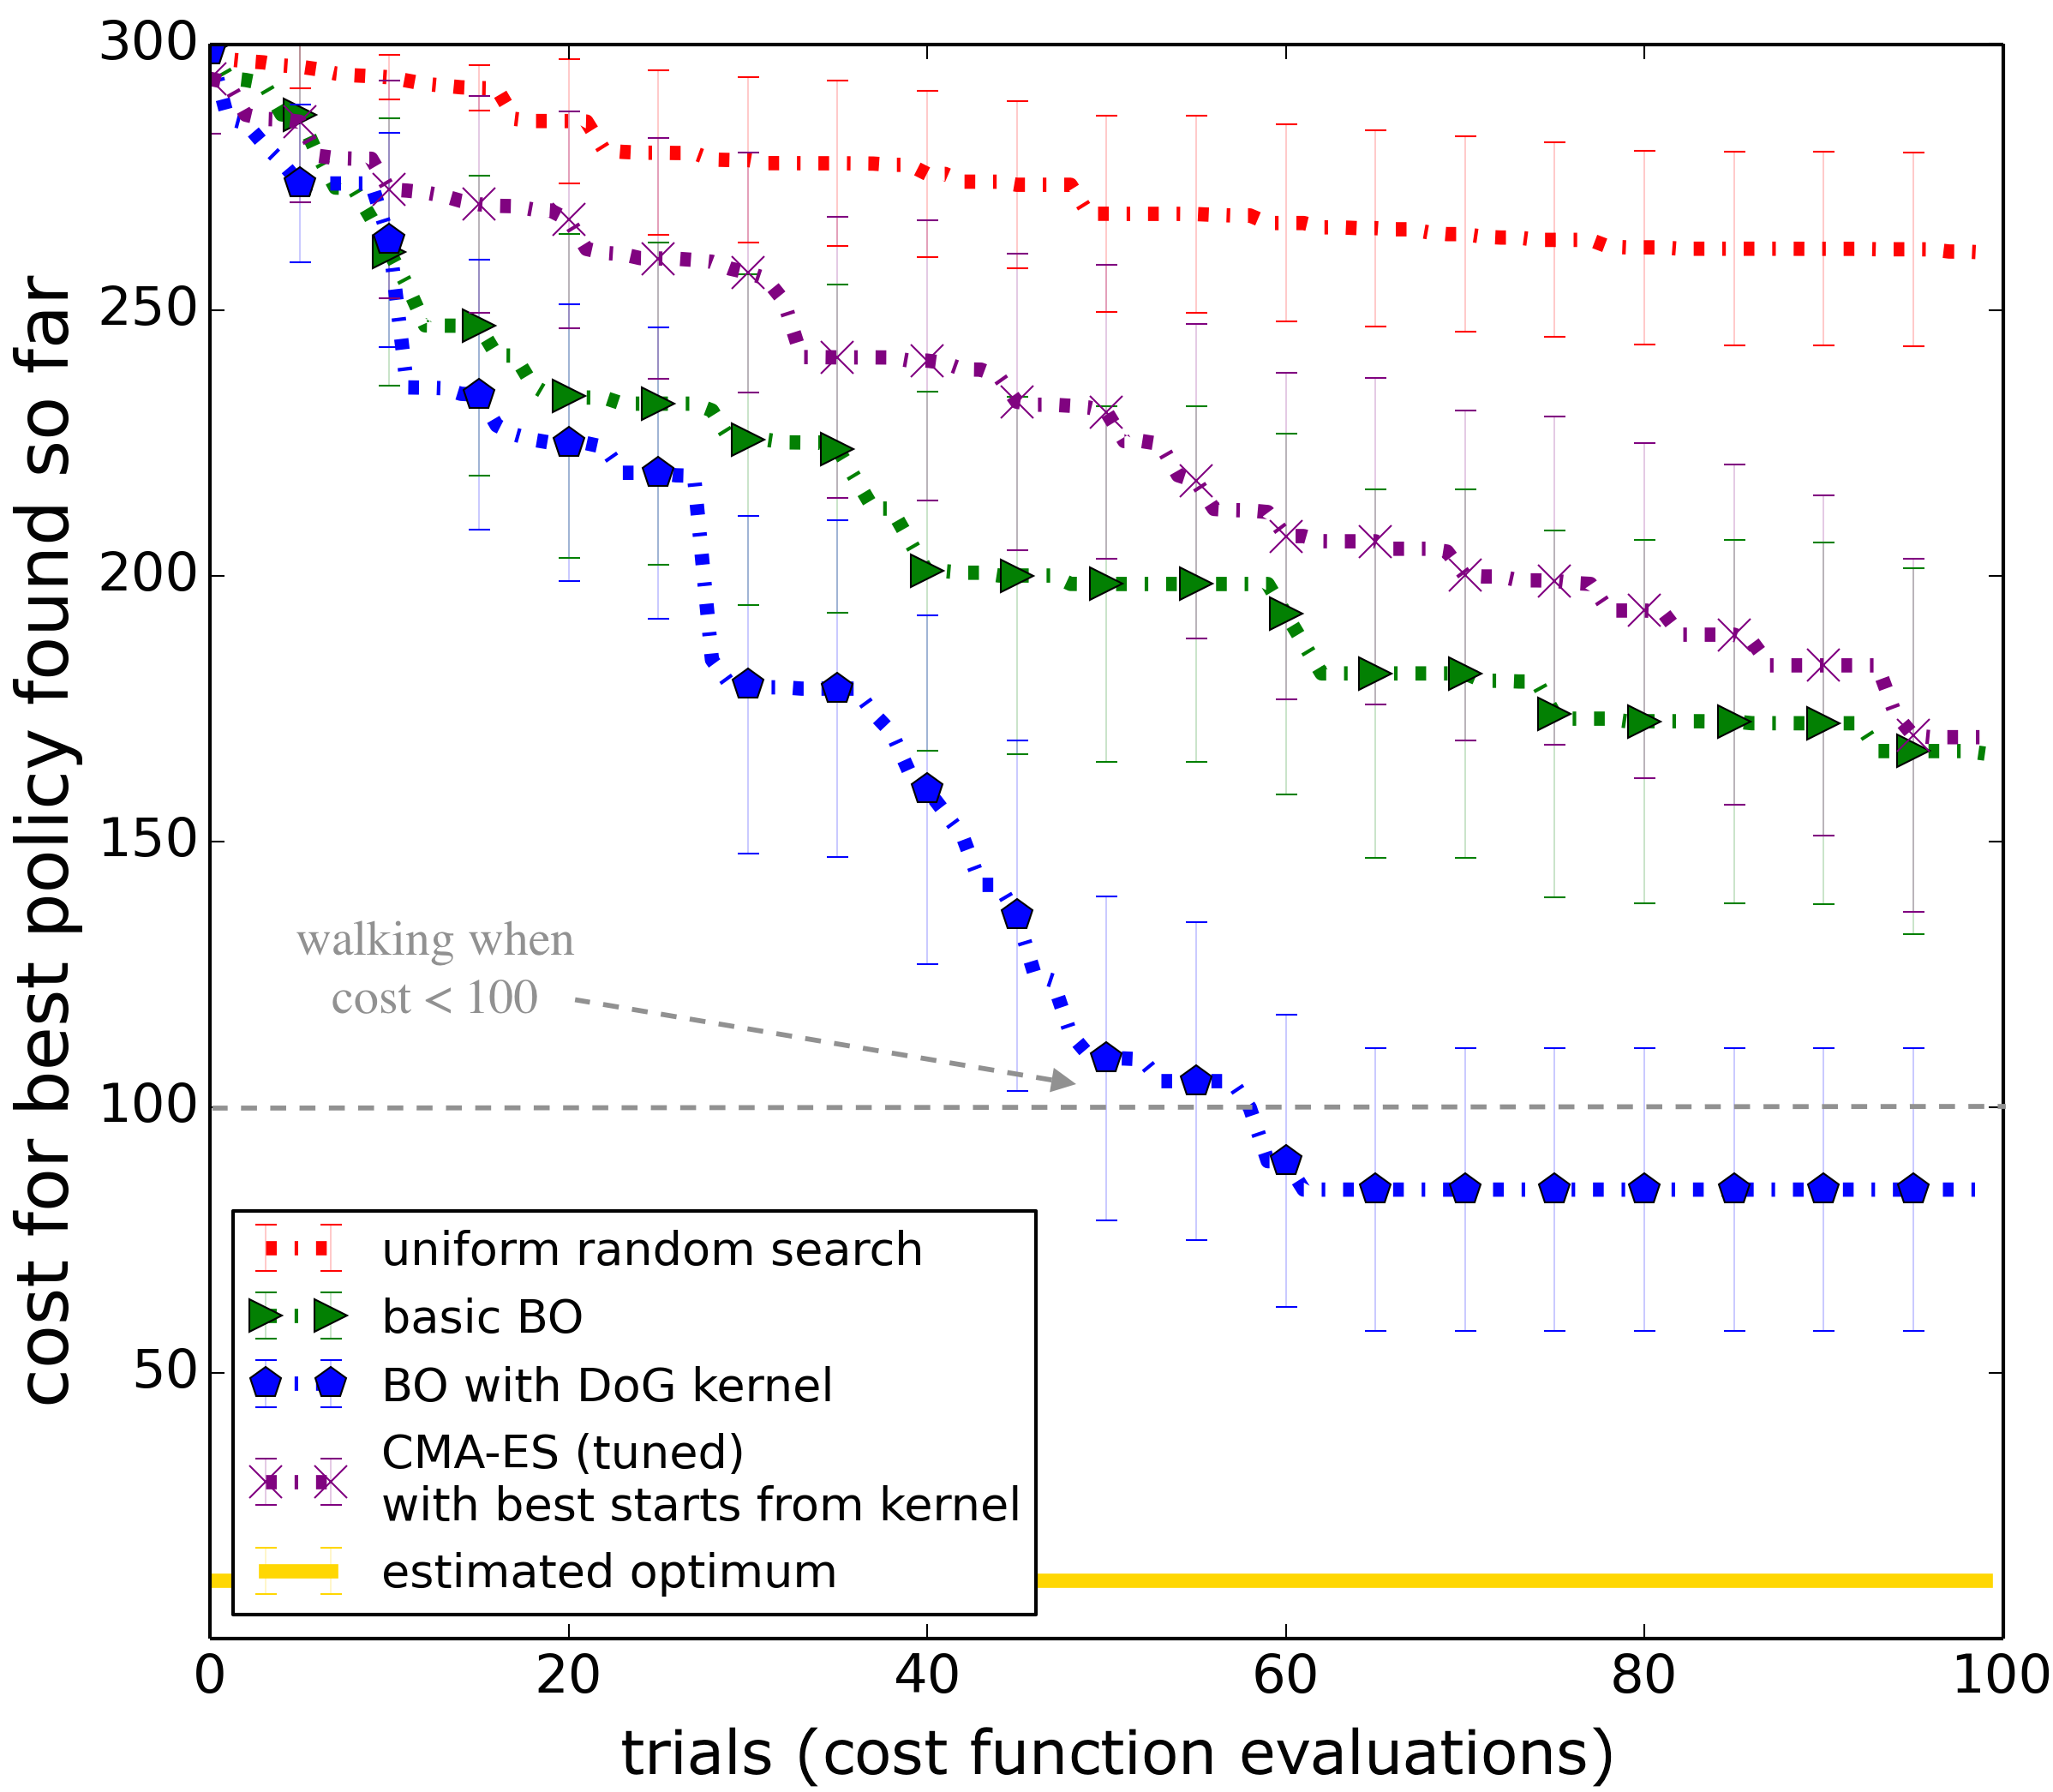
\includegraphics[width=0.6\textwidth]{img/rnd_bo_bo_covLoc_cma_rough6_disturb_nonsmooth_cost.png}
\caption{Experiments using \dogkernel kernel on rough ground with model disturbances on the non-smooth cost over 50 runs. Policies with costs below 100 generate walking behaviour for 100 seconds in simulation. None of the optimization methods find optimal policies in all the runs and hence the mean cost is higher than the estimated optimum.}
\label{fig_bo_locomotion_non_smooth}
\end{figure}

We observed good performance on the non-smooth cost function (Figure \ref{fig_bo_locomotion_non_smooth}), though it was not as remarkable as the smooth cost. BO with kernel still outperformed all other methods by a margin, but this different cost seems to hurt BO and \mbox{CMA-ES} alike. Since this cost is discontinuous, there is a huge discrepancy between costs for parameters that walk and those that don't. If no walking policies are sampled, BO learns little about the domain and samples randomly, which makes it difficult to find good parameters. Hence not all runs find a walking solution. BO was able to find successful walking in $74\%$ of cases on rough ground with $\pm 6 cm$ disturbance in less than 60 trials/evaluations. \mbox{CMA-ES} starting from a good kernel point was able to do it in $40\%$ of runs. 

This showed that our kernel was indeed independent of the cost function to an extent, and worked well on two very different costs. We believe that the slightly worse performance on the second cost is because of the cost structure, rather than a kernel limitation, as it still finds walking solutions for a significant portion of runs.  


\subsubsection{Experiments on different terrains}

\begin{figure}[t]
\centering
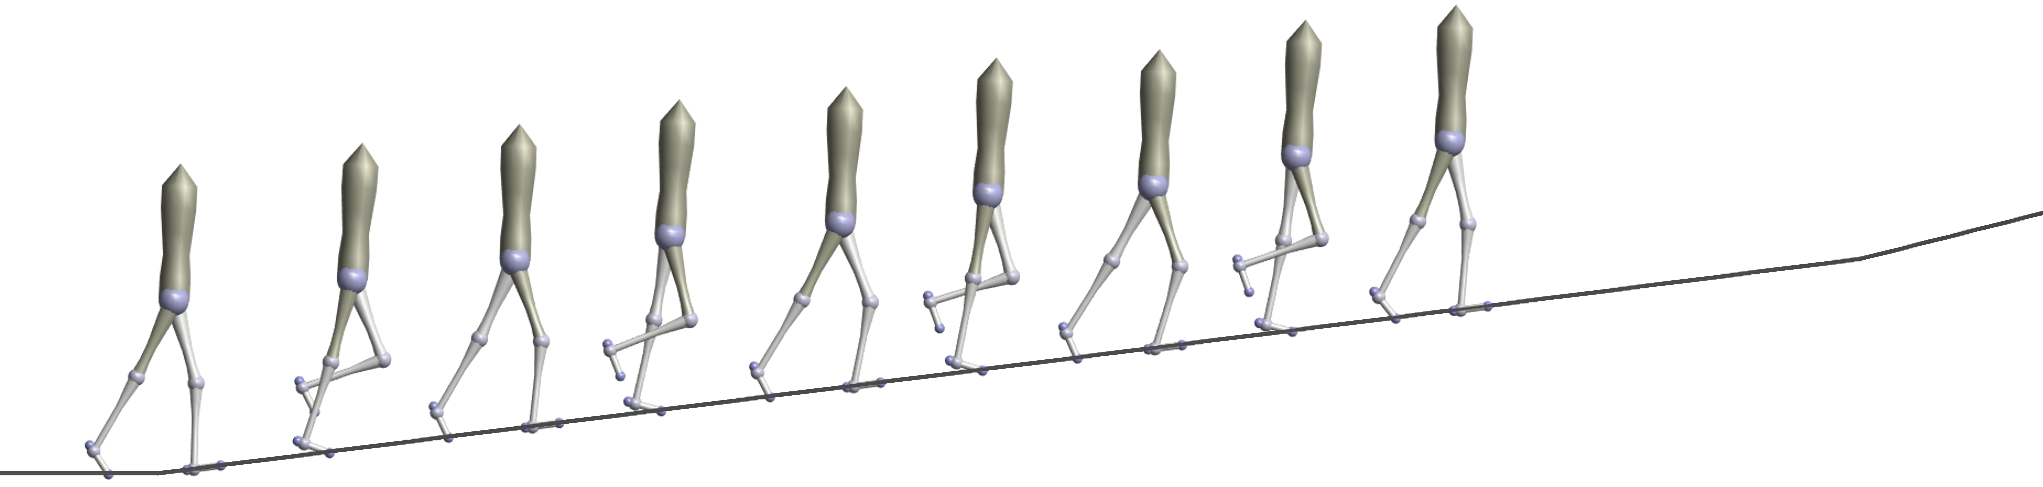
\includegraphics[width=0.8\textwidth]{img/rampup.png}
\vspace{10px}
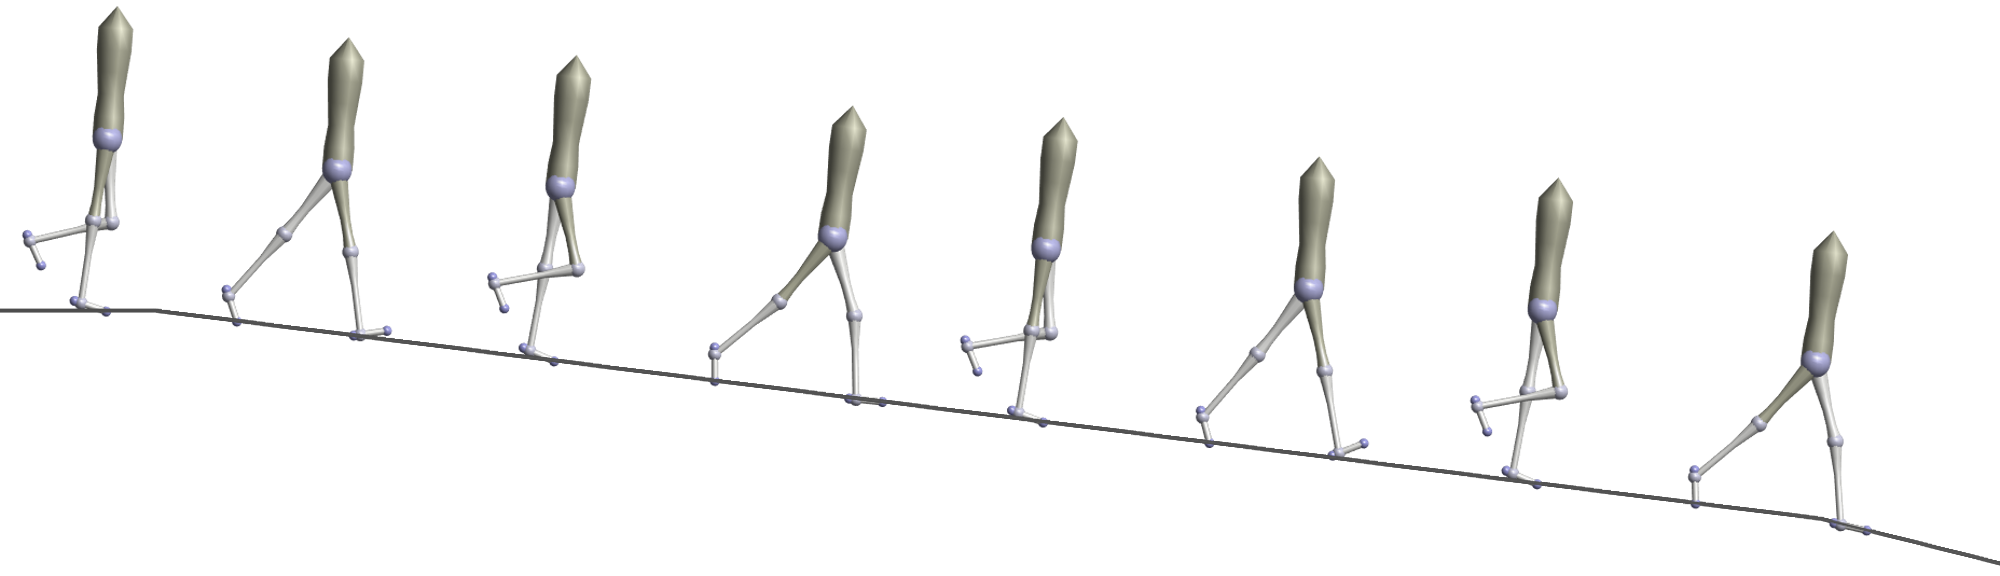
\includegraphics[width=0.8\textwidth]{img/rampdown.png}
\caption{Optimized policies walking up and down a $12.5 \%$ ramp.}
\label{fig_ramp}
\end{figure}

We also optimized on ramps -- sloping upwards, as well as downwards, with the kernel generated on flat ground. The ramp up and down ground slopes were gradually increased every $20m$, until the maximum slope was reached. The maximum slopes for going down and going up were $20\%$ ($tan(\theta) = 0.2, \theta=11.31\deg$). BO with DoG kernel was able to find parameters that walked for 100 seconds in $50\%$ of cases in ramp up and $90\%$ in ramp down. Example optimized policies walking up and down slope are shown in Figure \ref{fig_ramp}.

We believe the reason we could not find walking policies on ramps in all runs, was that we are not optimizing the hip lean, which was noted to be crucial for this profile in \cite{song2015neural}. Since we did not consider this variable when generating our 16 dimensional kernel, it was not trivial to optimize over it without re-generating the grid. Similarly, we found that we could not find any policies that climbed up stairs. Perhaps this could be achieved when optimizing over a much larger set of parameters, as in \cite{song2015neural}. 

To test if the hip lean indeed helps climb up a ramp, we hand-tuned the hip lean to be $15^{\deg}$, instead of the original angle of $6^{\deg}$ for which the kernel was generated. Indeed, our rate of success on walking on ramp up ground profile increased from $50\%$ to $65\%$. %For walking upstairs, we achieved $10\%$ success. 
This shows that the hip lean indeed helped walking on these terrains, and ideally we would like to optimize it along with the other parameters. Also, it shows that the \dogkernel kernel is robust to changes in parameters that were used to generate it. This is an important property, as parameters in the neuromuscular model are changed slightly for different experiments, for example the ground stiffness, initial conditions of the model, etc. If the kernel results hold across a variety of such conditions, we don't need to regenerate it.

%In the future, we would like to include more variables for optimizing over different terrains, and include them as part of the kernel. 

\subsection{Summary of experiments with the DoG transform}



\begin{table}[h!]
\centering
\ra{1.3}
\small{
\begin{tabular}{@{}rrrrr@{}} 
\toprule
Controller & Robot & Environment & Speed & Number of trials \\
Dimension & & & profile & for stable walking \\

\midrule

Non-smooth cost \\

5 & ATRIAS & Hardware & Variable & 3 \\

9 & ATRIAS & Hardware & Constant & 5 \\

9 & ATRIAS & Simulation & Constant & 9 \\

16 & 7-link & Simulation & Constant & 60 \\

50 & ATRIAS & Simulation & Constant & 10 \\

Smooth cost \\

16 & 7-link & Simulation & Constant & 25 \\

\bottomrule
\end{tabular}
}
\caption{Summary of experiments with DoG features in simulation and hardware on the ATRIAS biped and 7-link bipedal robot. All simulation experiments are conducted with un-modelled disturbances.}
\label{tbl:dog_expts_details}
\end{table}



\section{Experiments with the NN transform}

In this section we describe our experiments with cost-based and trajectory-based neural network kernels, described in Section \ref{sec:nn_transform}. We first consider the setting of optimizing a 5-dimensional controller for the ATRIAS robot from Section \ref{sec:raibert_cont}. We show that the cost-based kernel is able to improve sample efficiency over standard Bayesian Optimization. We present hardware experiments to demonstrate that our kernel allows obtaining a set of parameters close to optimal on the second trial for a constant target speed. With a variable target speed, it can find walking controllers reliably in 5 trials.

Next, we discuss simulation experiments with a 16 dimensional controller that utilizes a Neuromuscular model from Section \ref{sec:7_link_biped} on a 7-link biped. These experiments show that our trajectory-based kernel is able to significantly outperform standard Bayesian optimization for a higher-dimensional controller even when a sharply discontinuous cost is used during optimization.

\subsection{Hardware experiments with a 5-dimensional controller}
\label{experiments_atrias}

For our experiments on the ATRIAS robot we used a high-fidelity ATRIAS simulator from ~\cite{martin2015robust} to generate the data for learning the network. 
%We did an initial analysis of the performance of our approach in simulation, followed by hardware experiments. 
%Then we conducted a set of hardware experiments on the ATRIAS robot using a controller described in Section~\ref{sec:probform}. 
We constructed a distance metric for a kernel used in Bayesian Optimization by training a neural network to reconstruct cost obtained from short simulations. We created a sobol grid on the input parameter space with 20000 points and ran short 3.5 second simulations on each of the corresponding 20000 parameter sets to compute the costs. We then used a fully connected network with 4 hidden layers (128, 64, 16, 4 units) with L1 loss to reconstruct the transformation of the cost described in Section~\ref{sec:approach_asym}.


We sampled 100 random controllers with a target speed of $0.4m/s$ on hardware, and 16 controllers walked. A lower target speed meant that $\frac{1}{6}$ of the controller space was stable walking controllers. We completed 6 sets of runs of BO: 3 using \textit{asymNN} kernel and 3 using a standard SE kernel with 10 trials each, leading to a \mbox{total of 60 hardware experiments}. Figure~\ref{fig:bo_runs_plot_atrias_hw} shows the performance of BO with SE versus \textit{asymNN} kernel. SE obtains a stable walking solution on the 3rd trial in one run, and on the 4th trial in the two other runs. \textit{asymNN} kernel is able to find the best-performing set of parameters on the second trial in each of the 3 runs. This confirms that using \textit{asymNN} kernel offers an improvement over using SE kernel in this setting. We suggest that \textit{asymNN} reliably selects a successful point on the 2nd trial  because such points lie far from  poorly performing subspace of parameters (under the distance metric constructed with \textit{asymNN}). 

While both SE kernel and \textit{asymNN} kernels perform very well in this setting, the \textit{asymNN} kernel is more biased towards sampling stable points than the SE kernel, as shown in Figure \ref{fig:bo_runs_plot_atrias_hw}. In the three runs, \textit{asymNN} kernel samples 23 stable controllers out of 30, while SE kernel samples 15 stable controllers. This implies that the search for optimal controllers is biased towards safety in the case of \textit{asymNN} kernel. This is desirable as stable points are less likely to break the robot.

\begin{figure}[t]
\centering
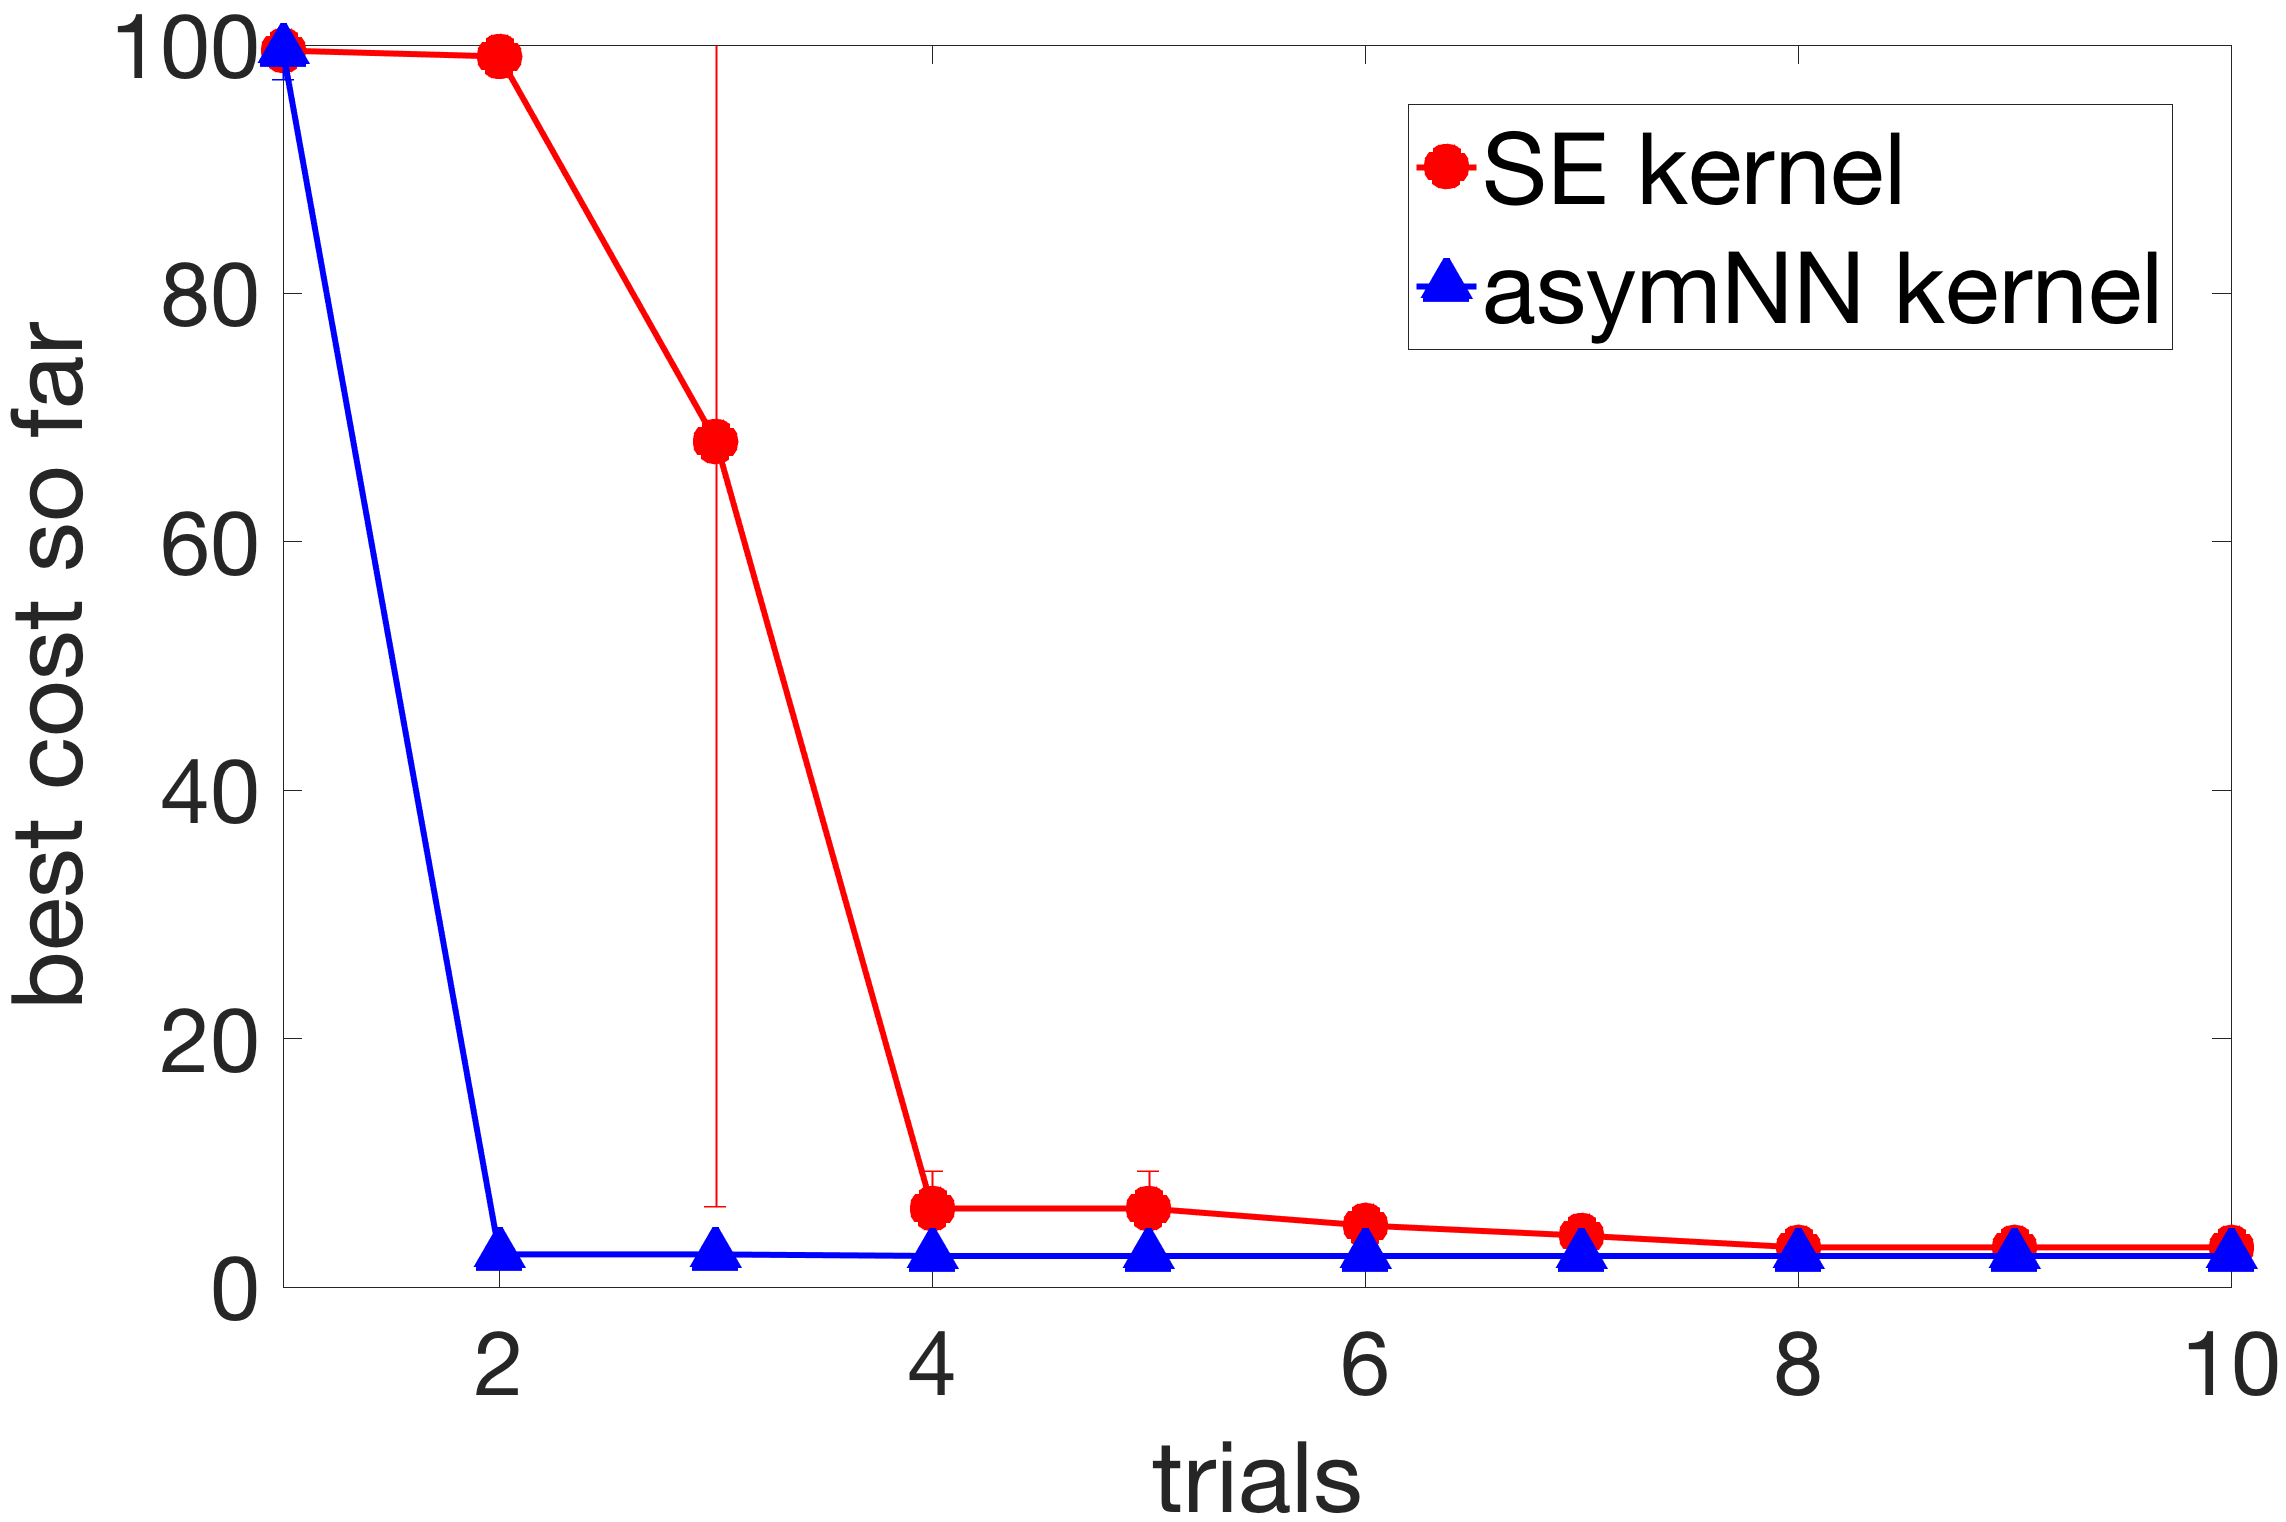
\includegraphics[width=0.43\textwidth]{img/hdw_runs.png}
\hspace{0.15cm}
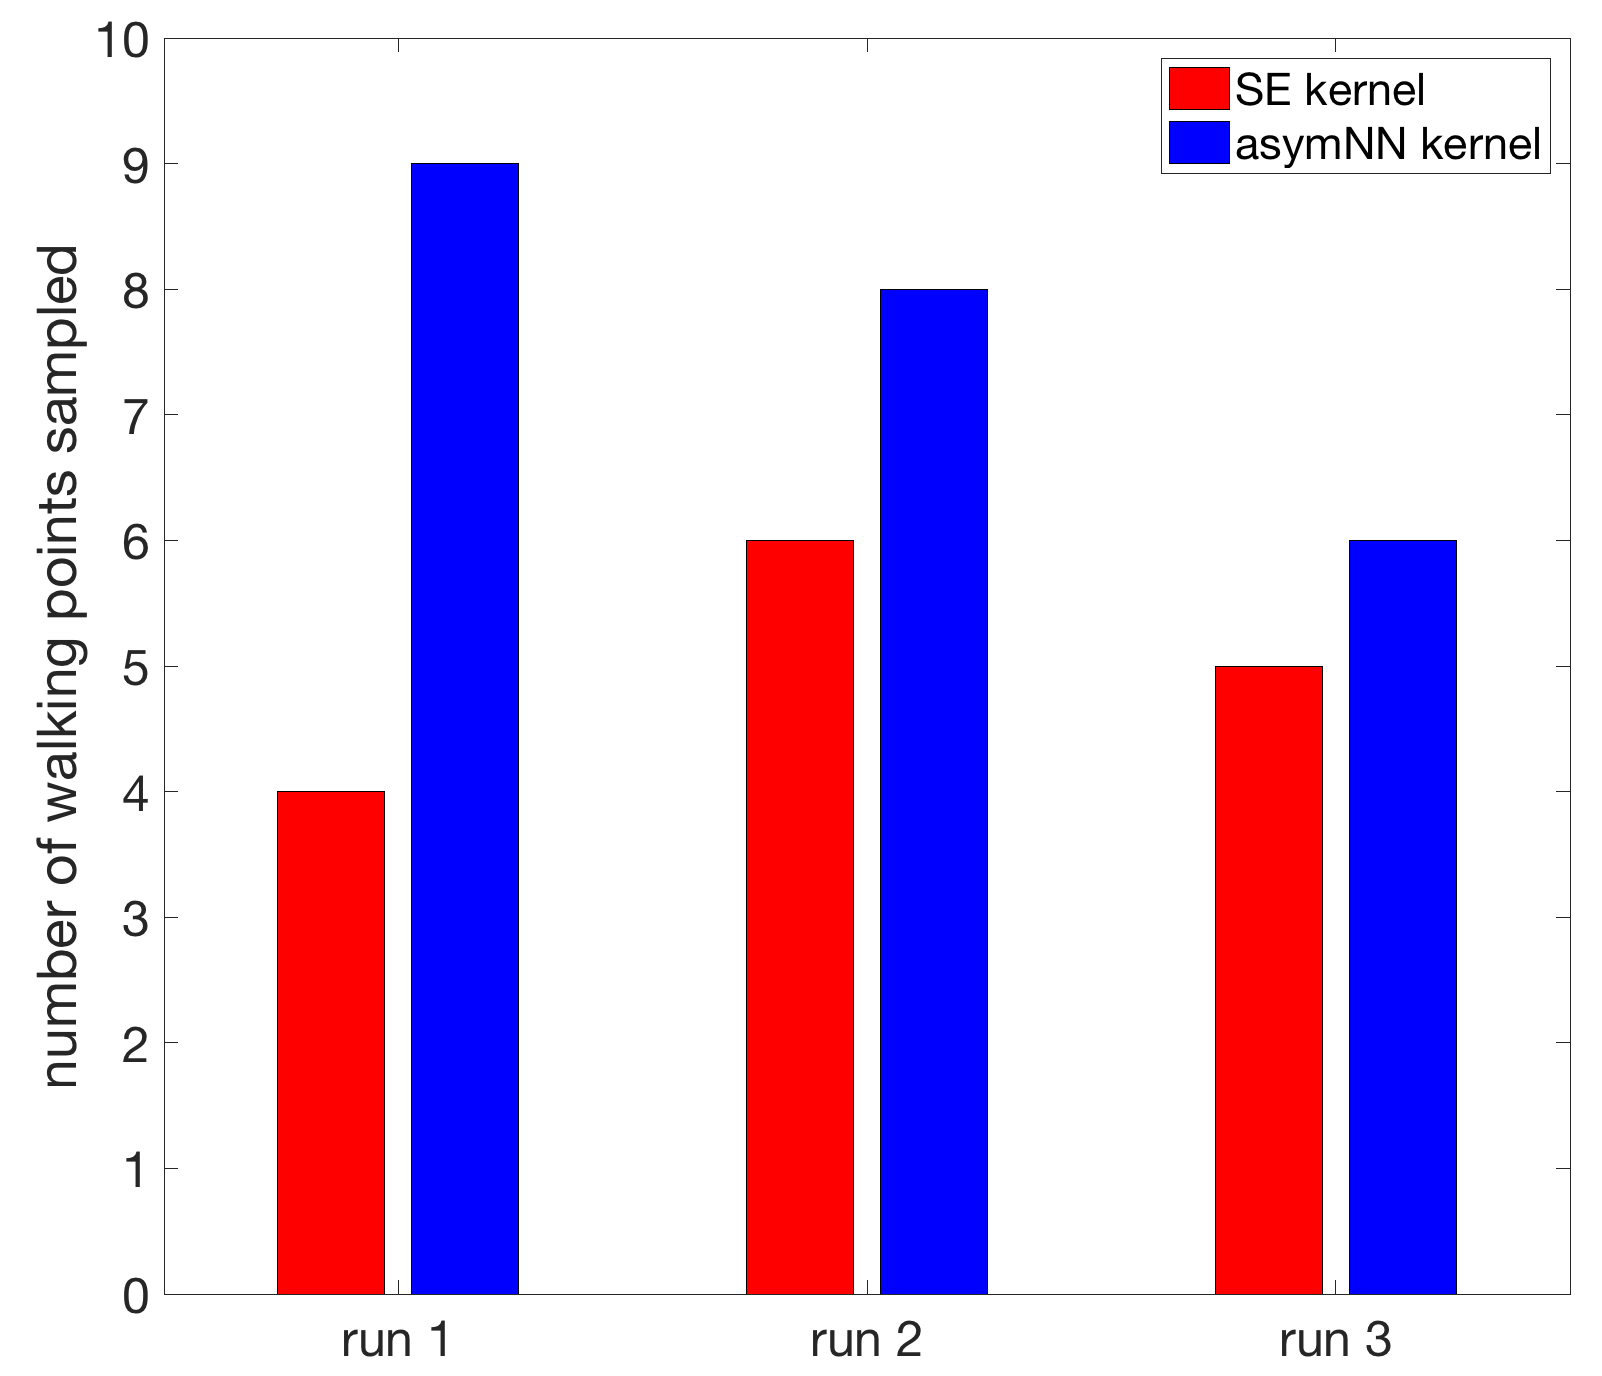
\includegraphics[width=0.43\textwidth]{img/walking_pts_sampled}
\caption{\small{(left) Best cost so far during BO (mean over 3 runs) for a target speed of $0.4m/s$. (right) Number of walking points sampled in each of the 3 runs.}}
\label{fig:bo_runs_plot_atrias_hw}
\end{figure}

On a more challenging, variable target speed profile of $0.4 m/s$ $\text{ (15 steps)} - 1.0 m/s \text{ (15 steps)} - 0.2 m/s \text{ (15 steps)} - 0 m/s \text{ (5 steps)}$, the performance of the \textit{asymNN} kernel is slightly worse than the \dogkernel, though still better than SE kernel. Figure \ref{fig:bo_nn_all_3} shows BO with  \textit{asymNN} kernel, SE kernel and \dogkernel for the variable speed profile. \dogkernel can find walking controllers in 2 trials in all 3 runs, while it takes \textit{asymNN} kernel 5 trials. On the other hand, SE kernel fails to reliably find controllers even after 20 trials.

\begin{figure}
    \centering
    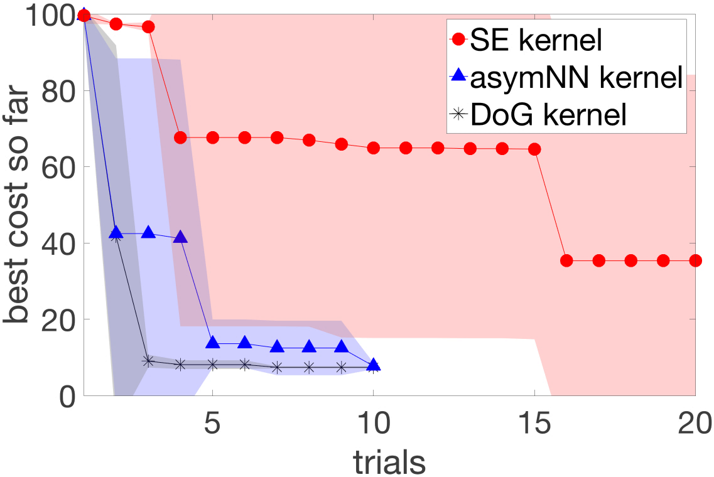
\includegraphics[width = 0.6\textwidth]{img/bo_nn_all_3.png}
    \caption{Bayesian optimization for a 5-dimensional controller with a variable target speed profile.}
    \label{fig:bo_nn_all_3}
\end{figure}


\begin{figure}[t]
\centering
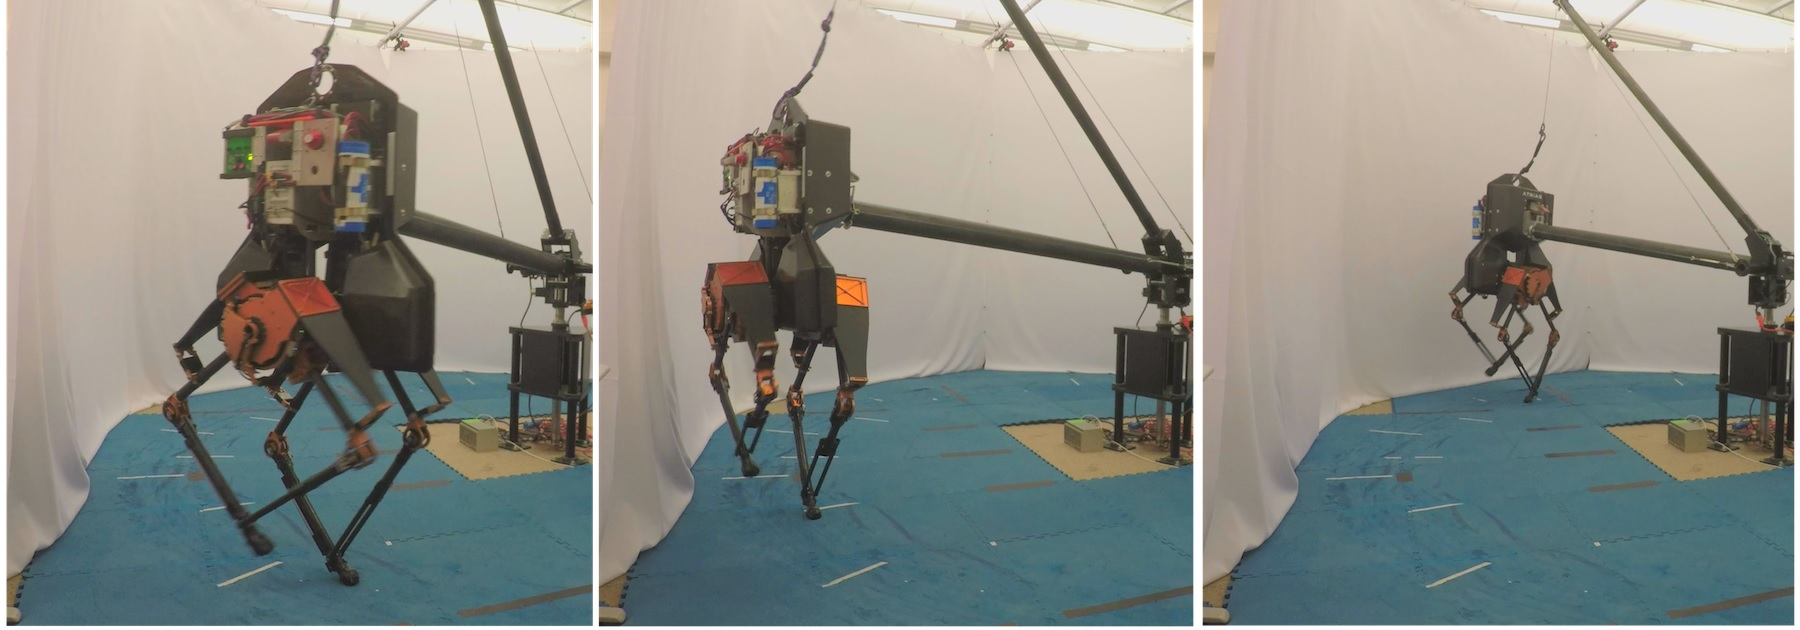
\includegraphics[width=0.8\textwidth]{img/atrias_walk_slides.jpg}
\caption{ATRIAS during BO with \textit{asymNN} kernel.}
\label{fig:bo_runs_atrias_hw_slides}
\end{figure}




While in our hardware setup most methods are likely to sample walking points within 10 trials, we believe our experimentation is an important step towards optimizing locomotion policies for complex humanoid robots. Bayesian Optimization studies in the past have also used real robot hardware, for example, \cite{Calandra2016}, \cite{cully2015robots} and \cite{tesch}.
However, \cite{tesch, lizotte2007automatic, cully2015robots} used robots which are statically stable for significant parts of their gait, making discontinuities in the cost function landscape less likely and in turn making the optimization easier. On the other hand, ATRIAS is a complex bipedal system which is likely to fall with unstable controllers due to point feet. \cite{Calandra2016} use a walking robot similar to ours. However, their controller parametrization is very different, and not widely used, unlike our inverse dynamics and force-based controller which is more modern and state-of-the-art \cite{kuindersma2016optimization}, \cite{herzog2016momentum}, \cite{feng2015optimization}. 

Hence, even if our policy parametrization was chosen so that steady walking points could be found in a few trials, our testbed is fairly complex and our problem formulation is widely applicable. 


\subsection{Hardware experiments with a 9-dimensional controller}

\begin{figure}
    \centering
    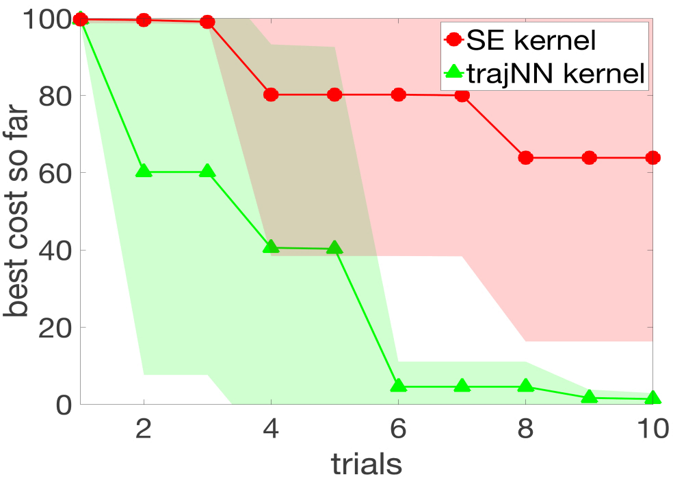
\includegraphics[width = 0.5\textwidth]{img/9d_hdw_nn.png}
    \caption{Bayesian optimization of a 9-dimensional controller with the \textit{trajNN} kernel.}
    \label{fig:9d_hdw_nn}
\end{figure}
In the next set of experiments, we evaluated performance of the \textit{trajNN} kernel described in Section~\ref{sec:approach_traj}. We optimize the 9-dimensional controller from Section \ref{sec:raibert_cont}. 

The target of hardware experiments was to walk for 30 steps at $0.4m/s$, similar to Section \ref{subsec:dog_9d}. We observed that the SE performance was slightly better as compared to the old experiments, even though starting from the same random samples, hyper-parameter setting and speed profile. We attribute this change to a better estimation and control of the CoM vertical height, owing to a new IMU on the robot. 


Figure~\ref{fig:9d_hdw_nn} shows comparison of BO with \textit{trajNN} kernel and SE kernels. We conducted 5 runs of both algorithms with 10 trials in each run, leading to a total of 100 robot trials. BO with the \textit{trajNN} kernel found walking points in all 5 runs within 6 trials, while BO with SE kernel only found walking points in 2 of 5 runs in 10 trials.
Hence, even without explicit hand-designed domain knowledge, like the \dogkernel kernel, the \textit{trajNN} kernel is able to extract useful information from simulation and successfully guide hardware experiments.


\subsection{Simulation experiments with the 16-dimensional controller}
\label{experiments_nm}

In section~\ref{sec:approach_traj} we introduced a cost-agnostic approach for constructing an informed kernel from simulations. Our approach is to train a neural network to reconstruct trajectory information. In this Section, we describe our experiments with 16 dimensional controller of the Neuromuscular model on a 7-link biped. We created a grid of 100K points in the input parameter space  and ran short 5 second simulations on each of the corresponding 100K parameter sets to collect the trajectory summaries. We then used a fully connected network with 4 hidden layers (512, 128, 32 units) with L1 loss to reconstruct the summaries of the trajectories (as described in section~\ref{sec:approach_traj}). This transformation induced by the neural network was used as a re-parameterization from the input space of 16-dimensional controller parameters to 8-dimensional space of trajectory summaries. These 8-dimensional outputs of the neural network define kernel distances in the informed kernel (\textit{trajNN}). All experiments were conducted on perturbed models, as described in Section \ref{sec:probform}.

Figures~\ref{fig:smooth_cost_bo_runs}, \ref{fig:nonsmooth_cost_bo_runs} illustrate our experiments comparing using \textit{trajNN} versus using Squared Exponential (\textit{SE}) kernel for BO. To analyze the performance of \textit{trajNN} on different cost functions we conducted experiments on two different costs suggested in prior literature. The first cost promotes walking further and longer before falling, while penalizing deviations from the target speed~\citep{rai2016sample}:
\begin{equation}
cost_{smooth} = 1/(1+t) + 0.3/(1+d) + 0.01(v-v_{tgt}),
\label{eq:cost_smooth}
\end{equation}
where $t$ is seconds walked, $d$ is the final hip position, $v$ is mean velocity and $v_{tgt}$ is the desired walking velocity ($1.3m/s$ in our case). 
The second cost function is a simplified version of the cost used in~\cite{song2015neural}, penalizes falls explicitly, and encourages walking at desired speed and with lower cost of transport:
\begin{equation}
cost_{non\text{-}smooth} = 		
    \begin{cases}
		300 - x_{fall} , \text{\small{if fall}} \\
		100 ||v_{avg} - v_{tgt}|| + c_{tr}, \text{\small{if walk}}\\
	\end{cases}
\label{eq:cost_nonsmooth}
\end{equation}
where $x_{fall}$ is the distance covered before falling, $v_{avg}$ is the average speed of walking, $v_{tgt}$ is the target velocity, and $c_{tr}$ captures the cost of transport.

Figure~\ref{fig:smooth_cost_bo_runs} shows that \textit{trajNN} offers a significant improvement in sample efficiency when using $cost_{smooth}$ during optimization. Points with cost less than $0.15$ correspond to robust walking behavior. With \textit{trajNN}, more than $90\%$ of runs obtain walking solutions after only 25 trials. In contrast, using \textit{SE} requires more than 90 trials for such success rate. The performance of \textit{trajNN} matches that of a \dogkernel kernel. This is notable, since \textit{trajNN} is learned automatically, whereas \dogkernel kernel is constructed using domain expertise.


\begin{figure}[t]
\centering
\caption{Optimizing smooth cost from Equation~\ref{eq:cost_smooth} over 50 runs.}
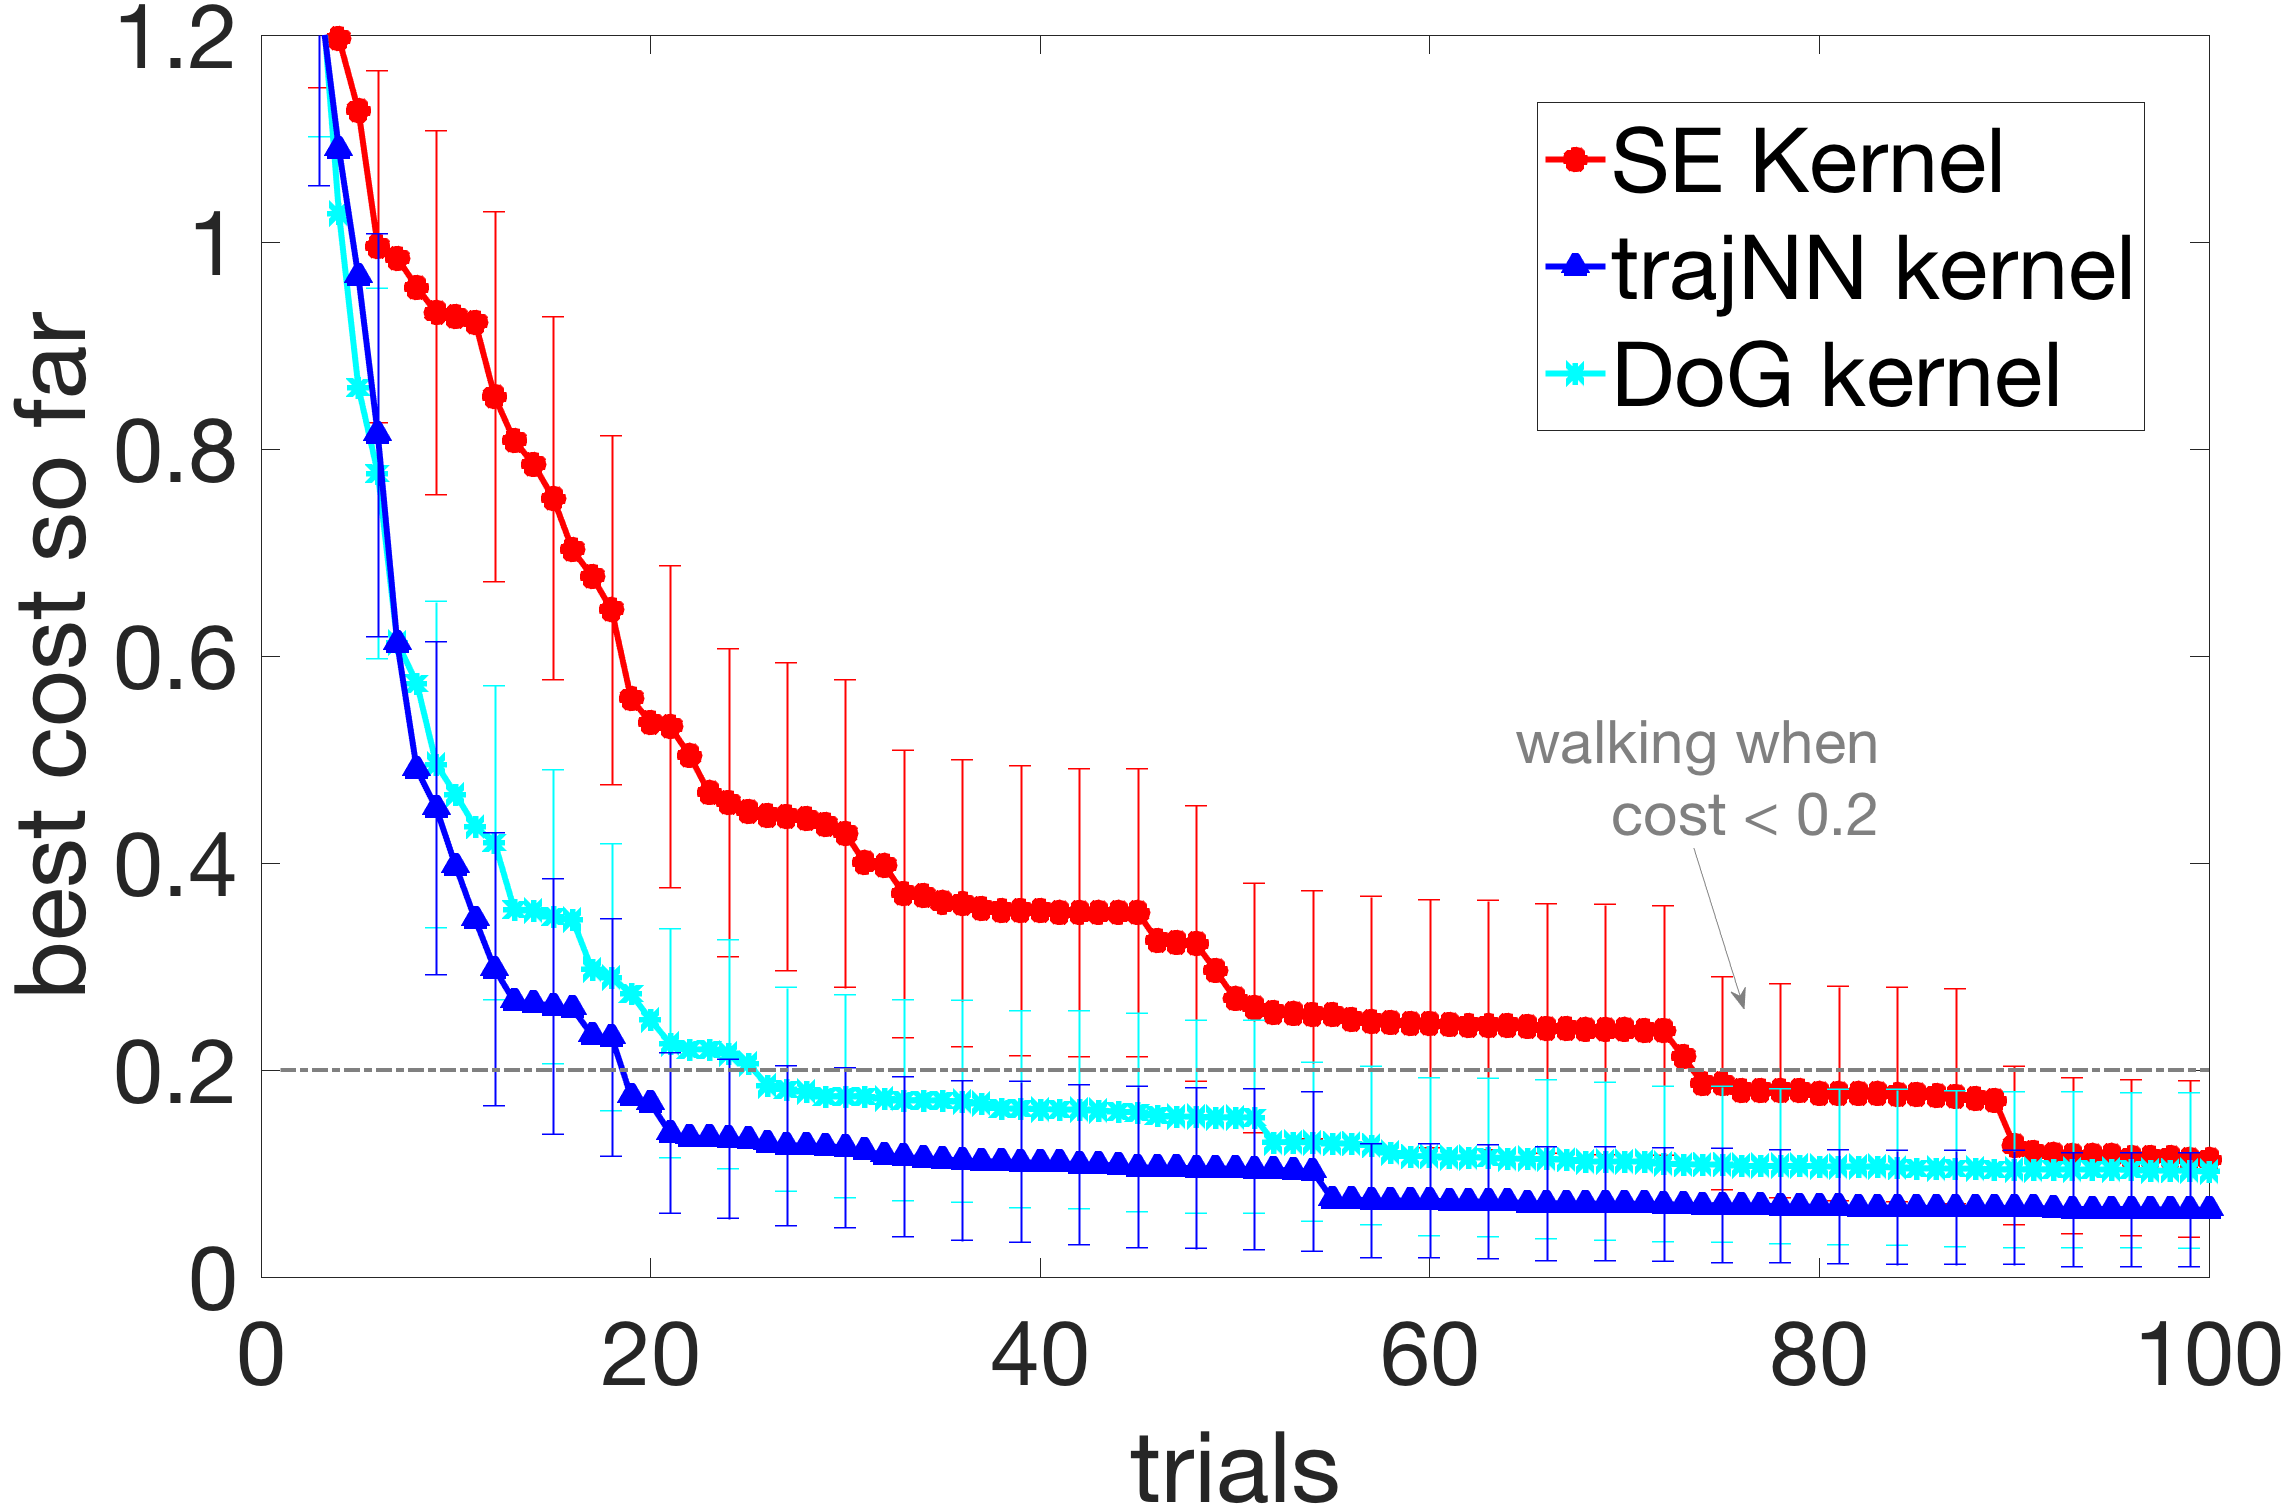
\includegraphics[width=0.65\textwidth]{img/smooth_cost_bo_runs}
\label{fig:smooth_cost_bo_runs}
\end{figure}

\begin{figure}[t]
\centering
\caption{Optimizing non-smooth cost from Equation~\ref{eq:cost_nonsmooth} over 50 runs.}
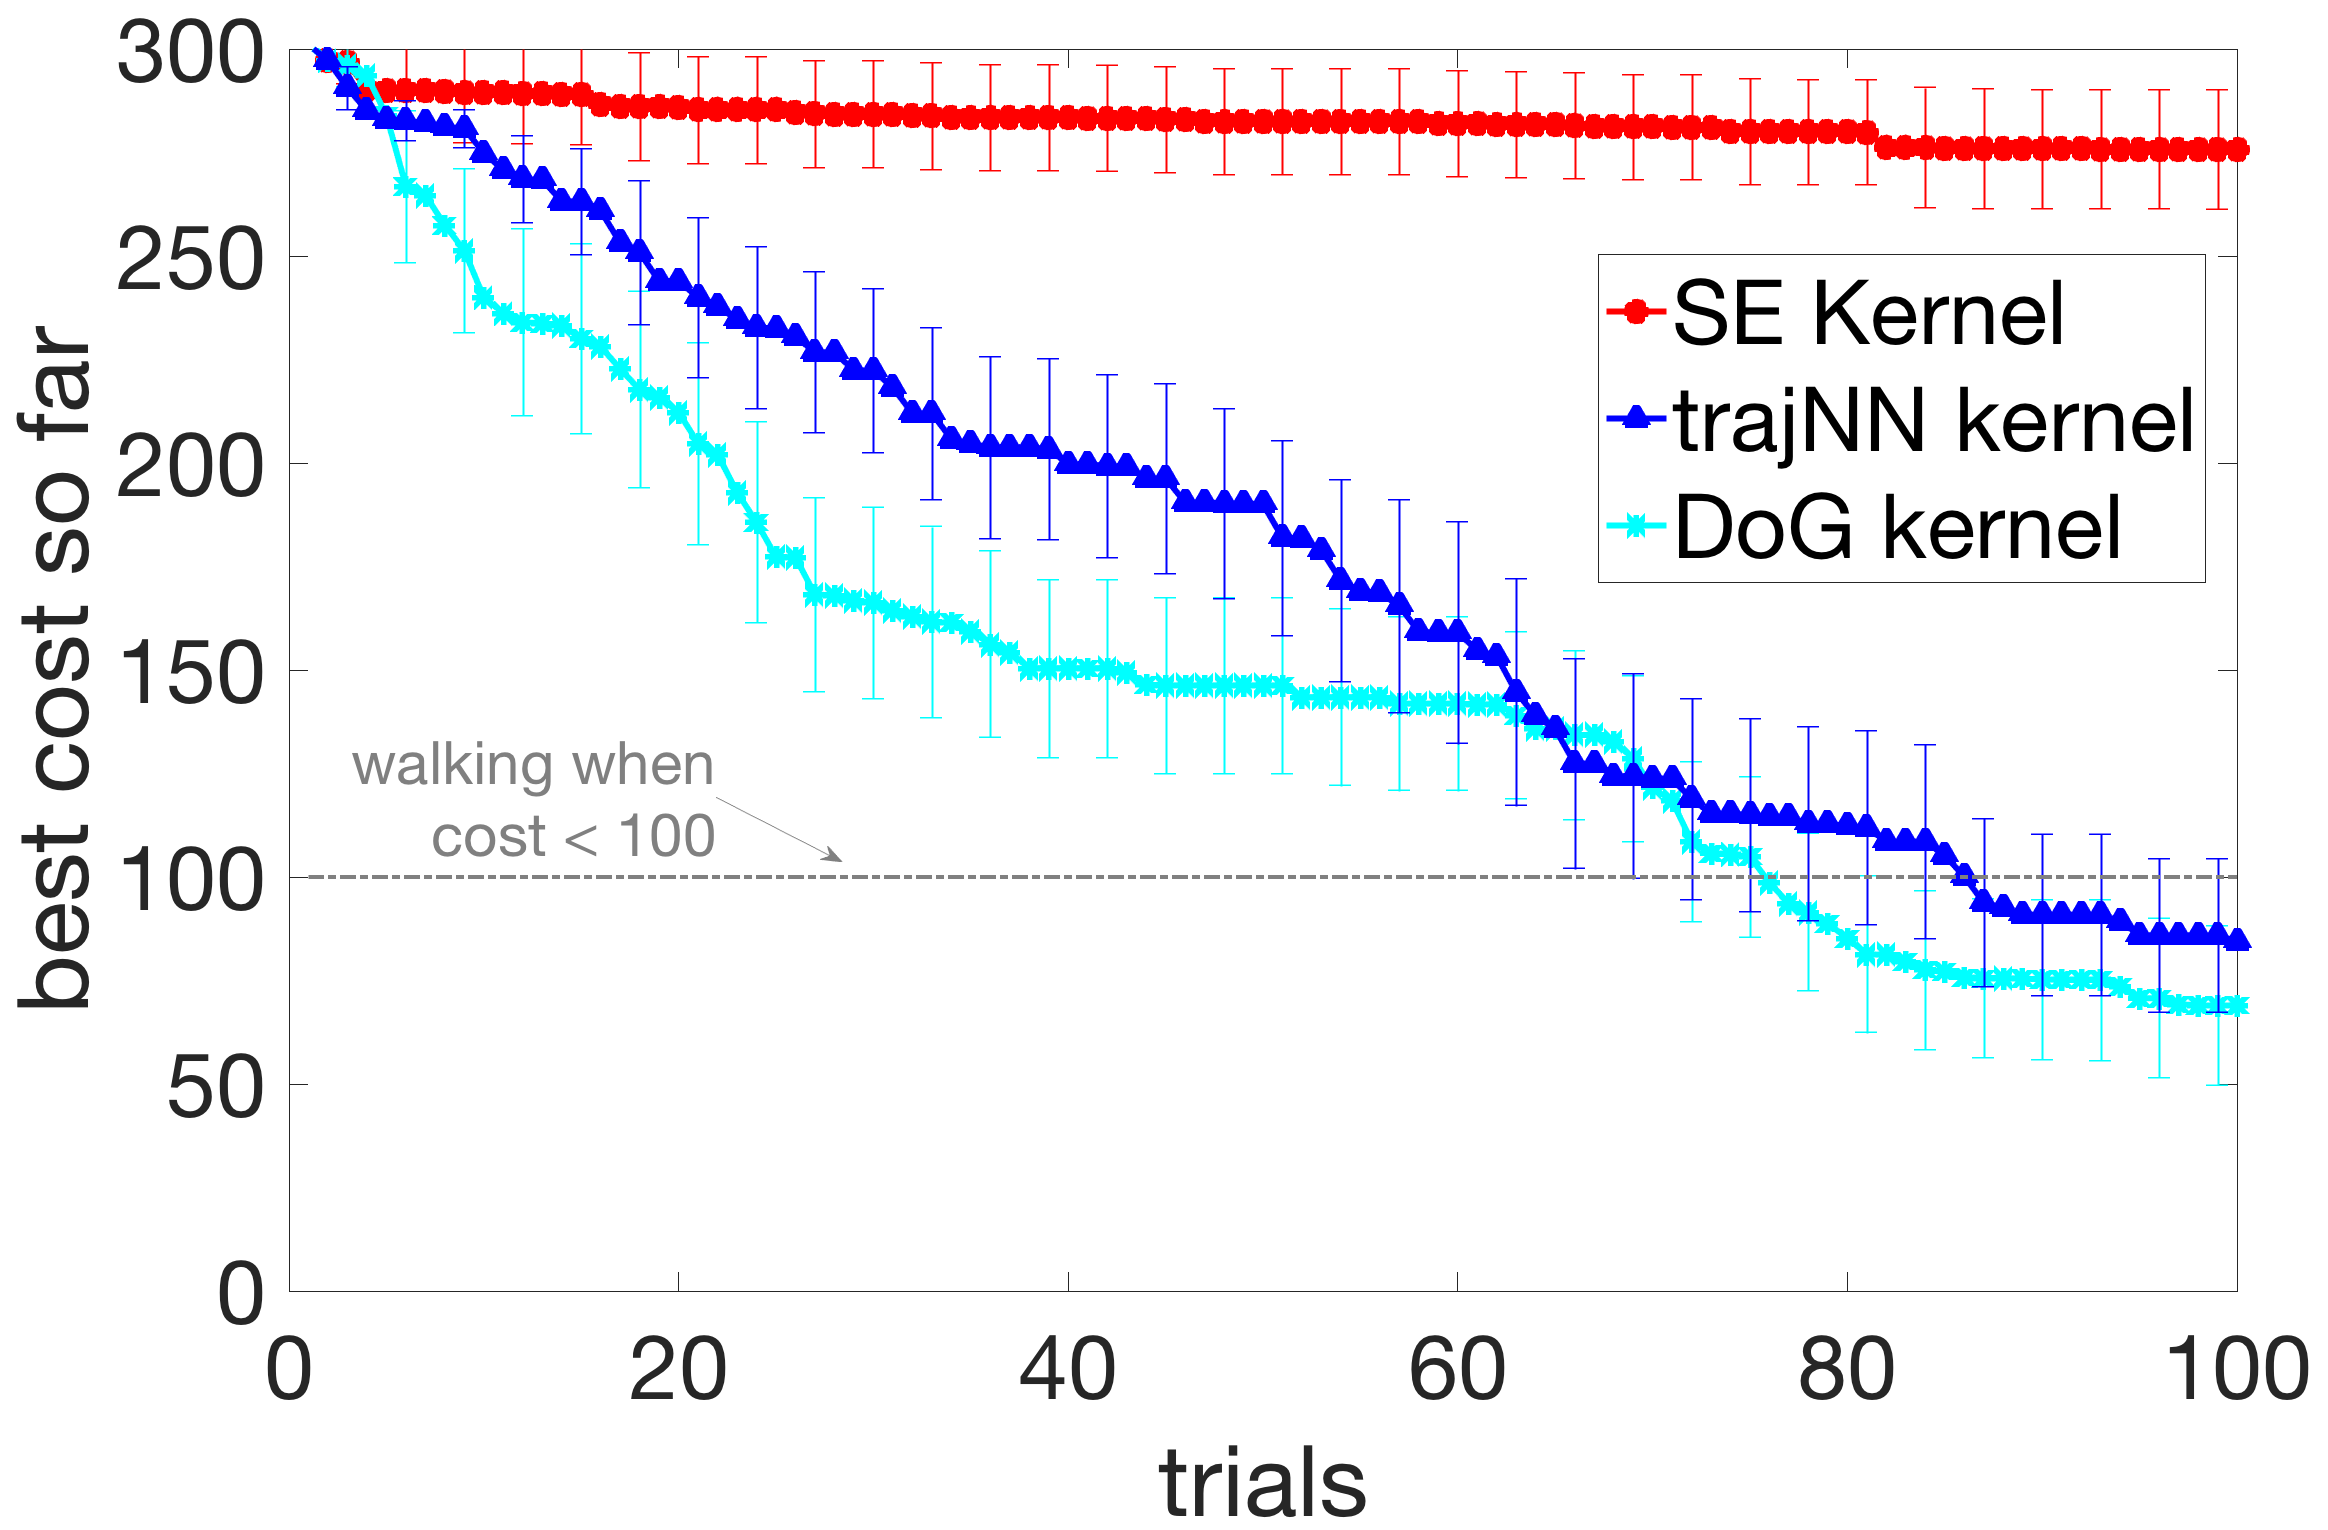
\includegraphics[width=0.65\textwidth]{img/nonsmooth_cost_bo_runs}
\label{fig:nonsmooth_cost_bo_runs}
\end{figure}

Figure~\ref{fig:nonsmooth_cost_bo_runs} shows that \textit{trajNN} also provides a significant improvement when using the second cost. Points with cost less than $100$ correspond to walking. With \textit{trajNN}, 70\% of the runs find walking solutions after 100 trials. In contrast, optimizing non-smooth cost is very challenging for BO with \textit{SE} kernel: a walking solution is found only in 1 out of 50 runs after 100 trials.

The difference in performance on the two costs is due to the nature of the two costs. If a point walks some distance $d$, Equation \ref{eq:cost_smooth} penalizes points according to $1/d$ and Equation \ref{eq:cost_nonsmooth} penalizes them according to $-d$. This results in a much steeper fall in cost with the first cost, and BO starts to exploit around points that walk some distance, quickly finding points that walk forever. However, with the second cost, BO continues to explore, and sometimes does not find walking points even in 100 trials. Exploitative methods might be better suited for higher dimensional problems, as compared to exploratory methods, in our experience. 

\textit{trajNN} kernel might be preferable to a cost-based kernel not only for settings with multiple costs. For some higher dimensional problems reduction to a 1-dimensional space in the kernel could be undesirable. So, while 1-dimensional cost-based kernel could yield highly sample-efficient optimization for lower dimensional problems, a higher-dimensional kernel like \textit{trajNN} could provide more flexibility without compromising sample-efficiency for higher dimensional problems.

\subsection{Simulation experiments with 50-dimensional controller}

\begin{figure}
    \centering
    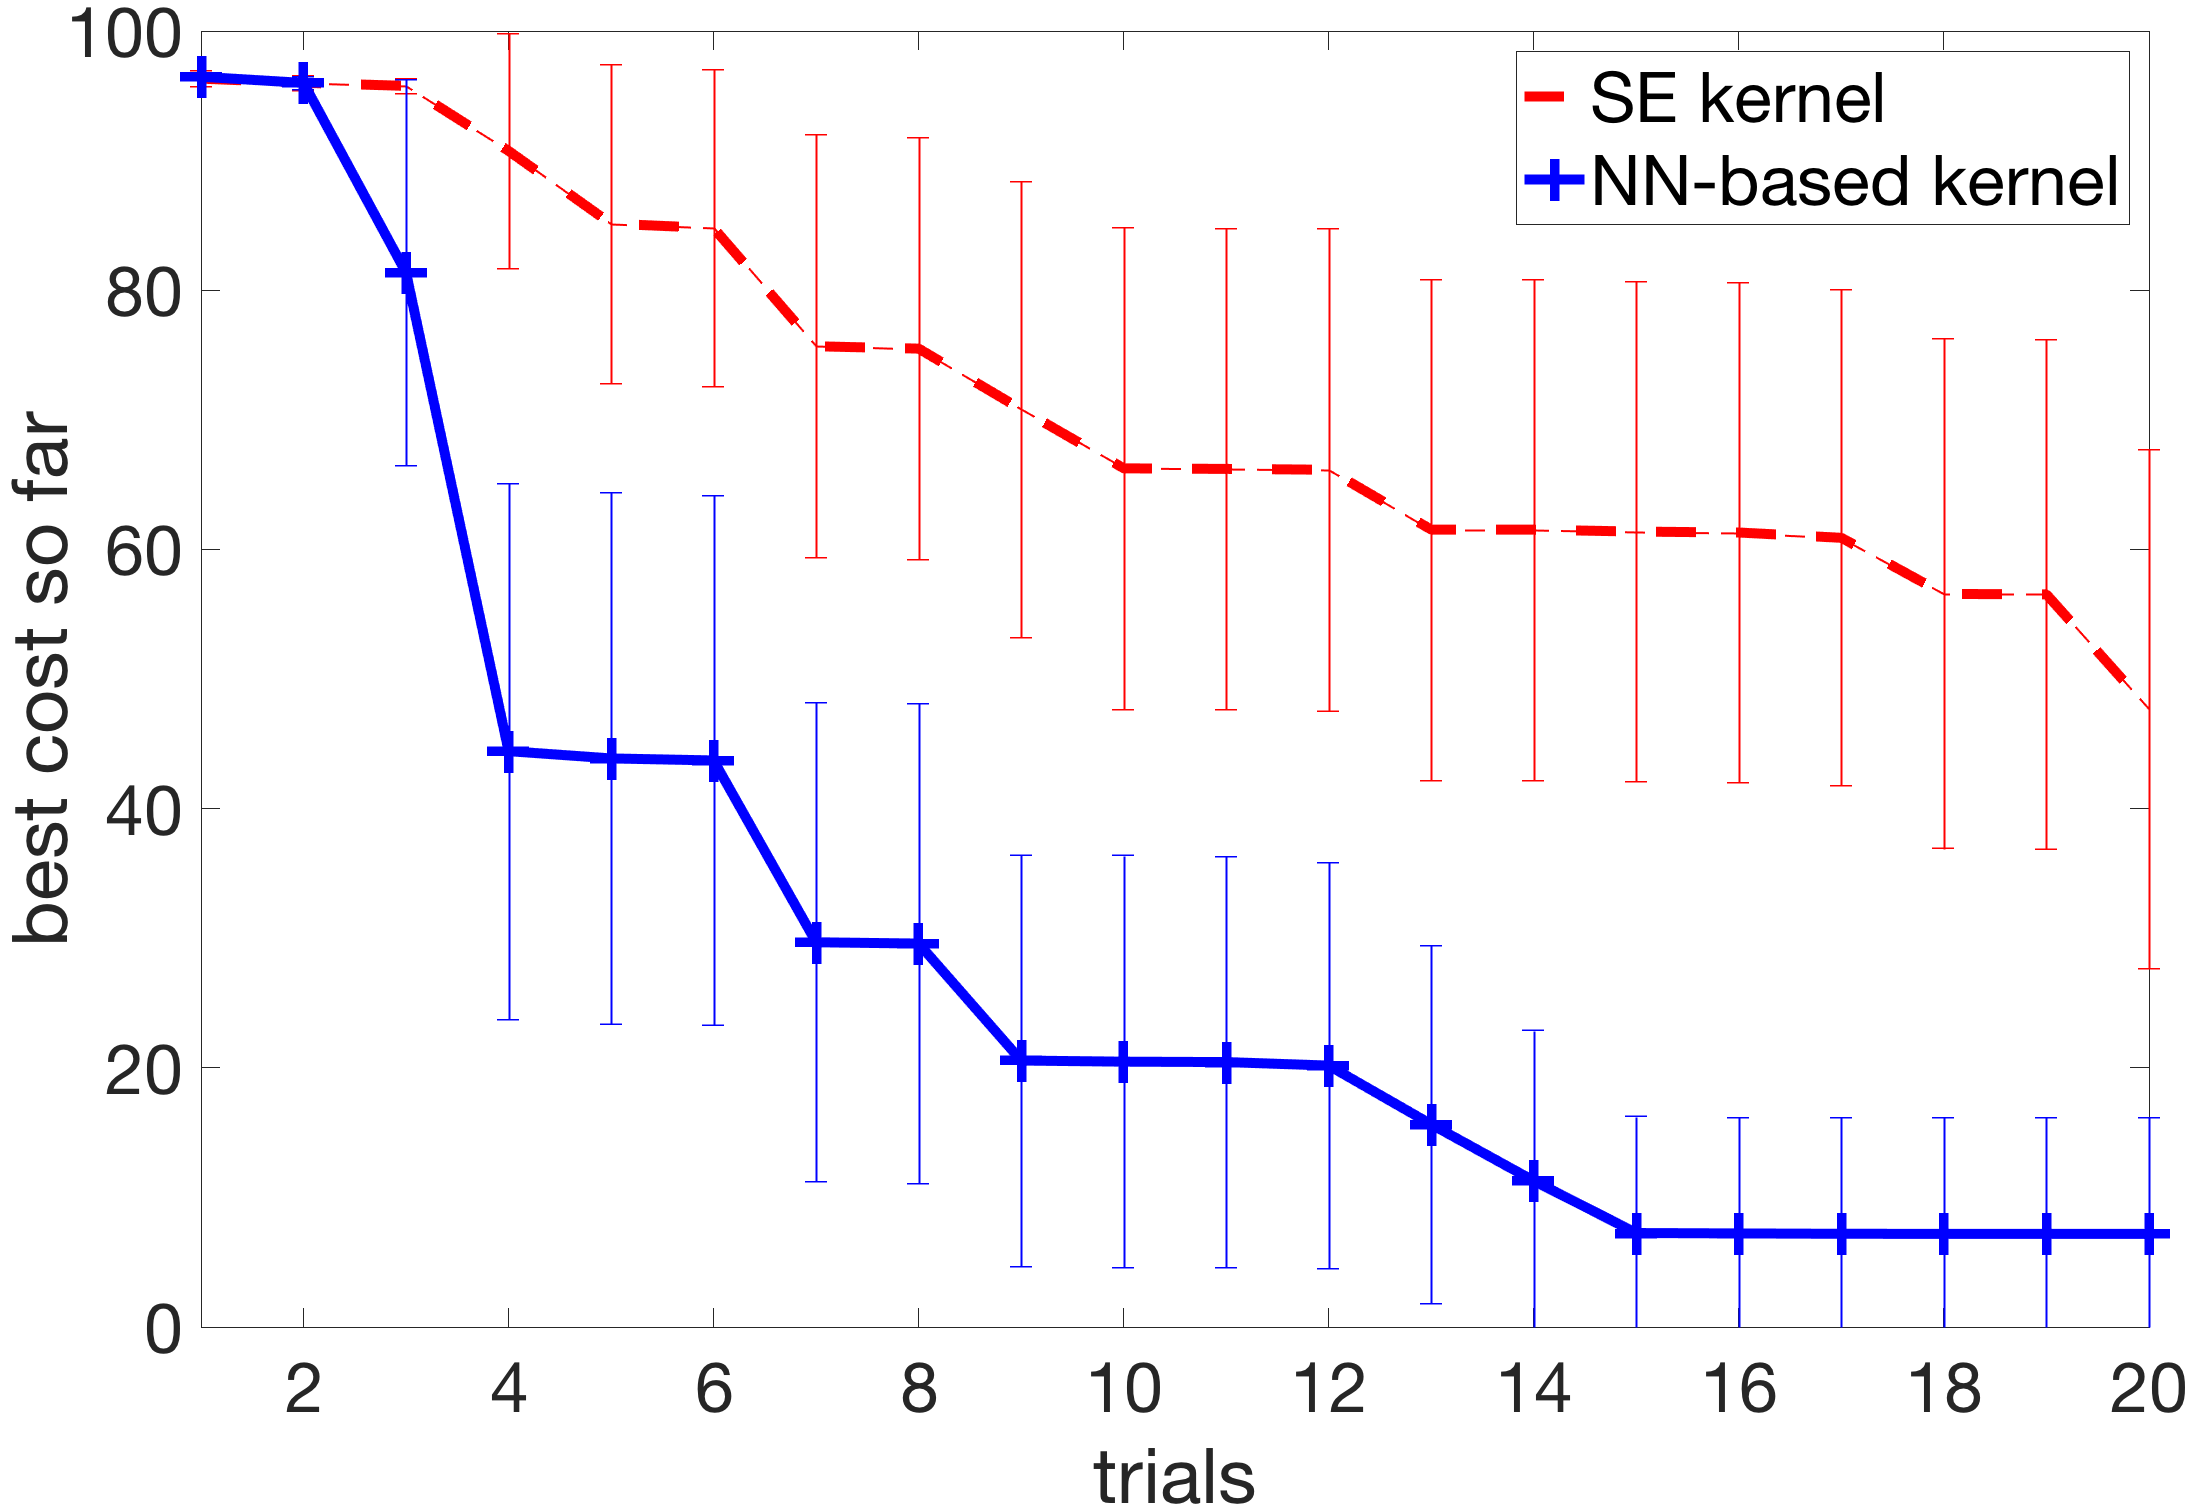
\includegraphics[width = 0.5\textwidth]{img/NN4_20runs_250K_holdout.png}
    \caption{50-dimensional controller with a \textit{trajNN} kernel in simulation.}
    \label{fig:nn4_vnmc}
\end{figure}

Our last set of simulation experiments were on the 50-dimensional controller, with the same experimental setting as Section \ref{sec:vnmc_expt}. The neural network kernel was trained to reconstruct the summaries of simulation trajectories over 200,000 simulation controllers. As can be seen in Figure \ref{fig:nn4_vnmc}, BO with NN-based kernel was able to find walking controllers in 20 trials in $95\%$ of the runs. This performance is similar to \dogkernel which can find walking controllers in 20 trials for $100\%$ of the runs. 

These results show that while the NN-based kernel uses lesser domain specific information than \dogkernel, its performance in simulation and hardware is very comparable to \dogkernel. As an additional advantage, the weights of the NN-based kernel can be learned from data experienced on hardware, by continuing to do gradient descent. This leads to a simple and straight-forward way of updating the kernel from hardware experiments. 

A summary of results and experimental settings described in the previous section is below:

\begin{table}[h!]
\centering
\ra{1.3}
\small{
\begin{tabular}{ lccccc } 
\toprule
Kernel & Controller & Number of & Sim & Kernel & Features \\
type & dimension & sim points & duration & dim & in kernel \\
\midrule
$k_{DoG}$ & 5 & 20K & 3.5s & 1 & $score_{DoG}$ \\ 
          & 9 & 100K & 5s & 1 & $score_{DoG}$ \\ 
     & 50 & 200K & 5s & 1 & $score_{DoG}$ \\ 
\hline
$k_{\textit{trajNN}}$ & 9 & 100K & 5s & 4 & $t_{walk}$, $x_{end}$, $\theta_{avg}$, $v_{x,avg}$\\ 
                      & 16 & 100K & 5s & 8 &
                $t_{walk}$, $x_{end}$, $\theta_{end}$, $v_{x,end}$\\
                & & & & & $c_{\tau}$,  $y_{end}$,  $v_{y,end}$, $\dot{\theta}_{end}$ \\ 
                      & 50 & 200K & 5s & 13 & $t_{walk}$, $x_{end}$, $c_{\tau}$, $\pmb{\textit{traj}}_{x}$, $\pmb{\textit{traj}}_{\theta}$ \\ 
\bottomrule
\end{tabular}
}
\caption{Simulation Data Collection Details. $score_{DoG}$ was described in Section \ref{sec:dog_transform}. For $k_{\textit{trajNN}}$: $t_{walk}$ is time walked in simulation before falling, $x_{end}$ and $y_{end}$ are the $x$ and $y$ positions of Center of Mass (CoM) at the end of the short simulation, $\theta$ is the torso angle, $\dot{\theta}$ is the torso velocity, $v$ is the CoM speed ($v_{x}$ is the horizontal and $v_y$ is the vertical component), $c_{\tau}$ is the squared sum of torques applied; $\pmb{\textit{traj}}_{x}$, $\pmb{\textit{traj}}_{\theta}$ denote vectors with mean CoM and $\theta$ measurements every second.}
\label{tbl:kernel_details}
\end{table}


\begin{table}[h!]
\centering
\ra{1.3}
\small{
\begin{tabular}{@{}rrrrrr@{}} 
\toprule
Controller & Robot & NN kernel & Environment & Speed & Number of trials \\
Dimension &        & Dimension &              & profile & for stable walking \\

\midrule

Non-smooth cost \\

5 & ATRIAS & 1 & Hardware & Constant & 2 \\

5 & ATRIAS & 1 & Hardware & Variable & 5 \\

9 & ATRIAS & 4 & Hardware & Constant & 6 \\

16 & 7-link &8 & Simulation & Constant & 90 \\

50 & ATRIAS &13 & Simulation & Constant & 15 \\

Smooth cost \\

16 & 7-link & 8 & Simulation & Constant & 50 \\

\bottomrule
\end{tabular}
}
\caption{Summary of experiments with neural network features in simulation and hardware on the ATRIAS biped and 7-link bipedal robot. All simulation experiments are conducted with un-modelled disturbances.}
\label{tbl:nn_expts_details}
\end{table}

\section{Effect of inaccurate simulations on the performance}

\label{subsec:mismatch_experiments}

%\begin{figure}
%\centering
%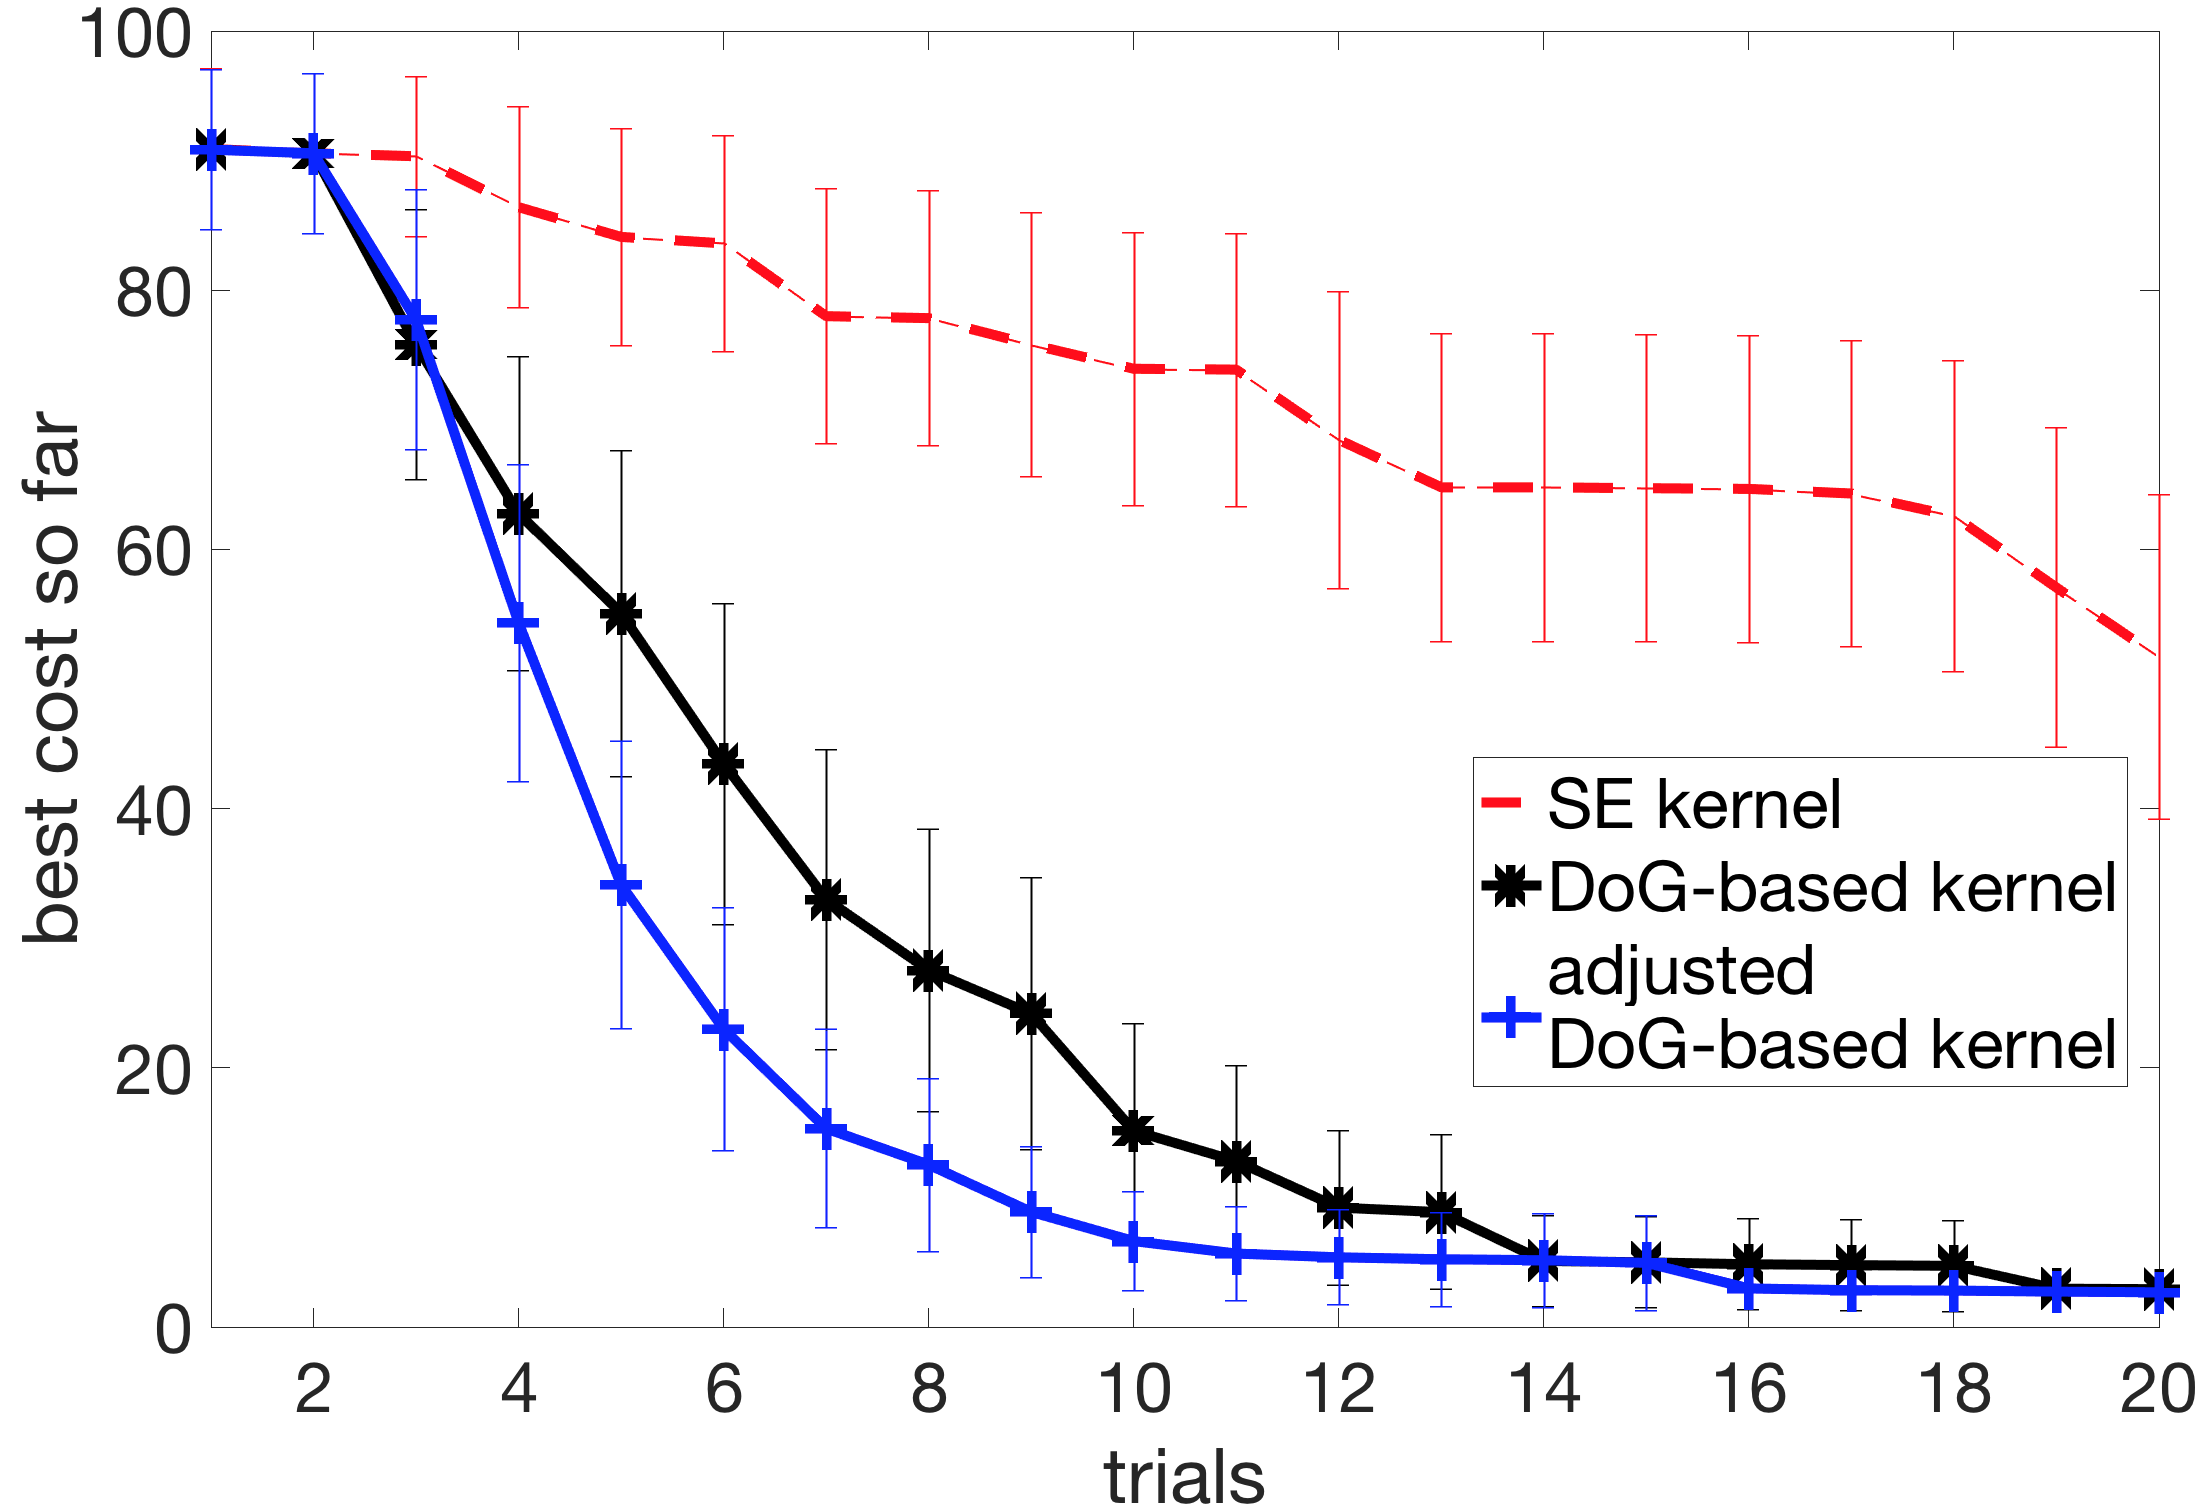
\includegraphics[width=0.5\textwidth]{img/sim_NM_Atrias_50d.png}
%\caption{\small{BO for 50d controller on original ATRIAS simulation.}}
%\label{fig:50d_sim}
%\end{figure}

In this section, we describe our experiments with increasing simulation-hardware mismatch and its effect on approaches that use information from simulation during hardware optimization. The quality of information transfer between simulation and hardware depends not only on the mismatch between the two, but also on the controller used. For a robust controller, small dynamics errors would not cause a significant deterioration in performance, while for a sensitive controller this might be much more detrimental. There is still an advantage to studying such a sensitive controller, as it might be much more energy efficient and versatile. In our experiments, the 50-dimensional VNMC described in Section \ref{sec:VNMC_cont} is capable of generating very efficient gaits but is sensitive to modelling errors. Figure \ref{fig:sim_NM_Atrias_50d} shows the performance of the DoG-based and adjusted DoG-based kernel on the original high-fidelity simulator. While both methods find walking points in 20 trials, adjusted-DoG performs better. There is mismatch even between short $5s$ and long $30s$ simulations for this controller. This mismatch is compensated by the adjusted-DoG kernel.


In the rest of this section, we provide experimental analysis of settings with increasing simulated mismatch and their effect on optimization of the 50-dimensional VNMC. We compare several approaches that improve sample-efficiency of BO and investigate if the improvement they offer is robust to mismatch between the simulated setting used for constructing kernel/prior and the setting on which BO is run. 

\subsection{Incorrect dynamics models}
\begin{figure}[t]
\begin{subfigure}[t]{0.47\textwidth}
\centering
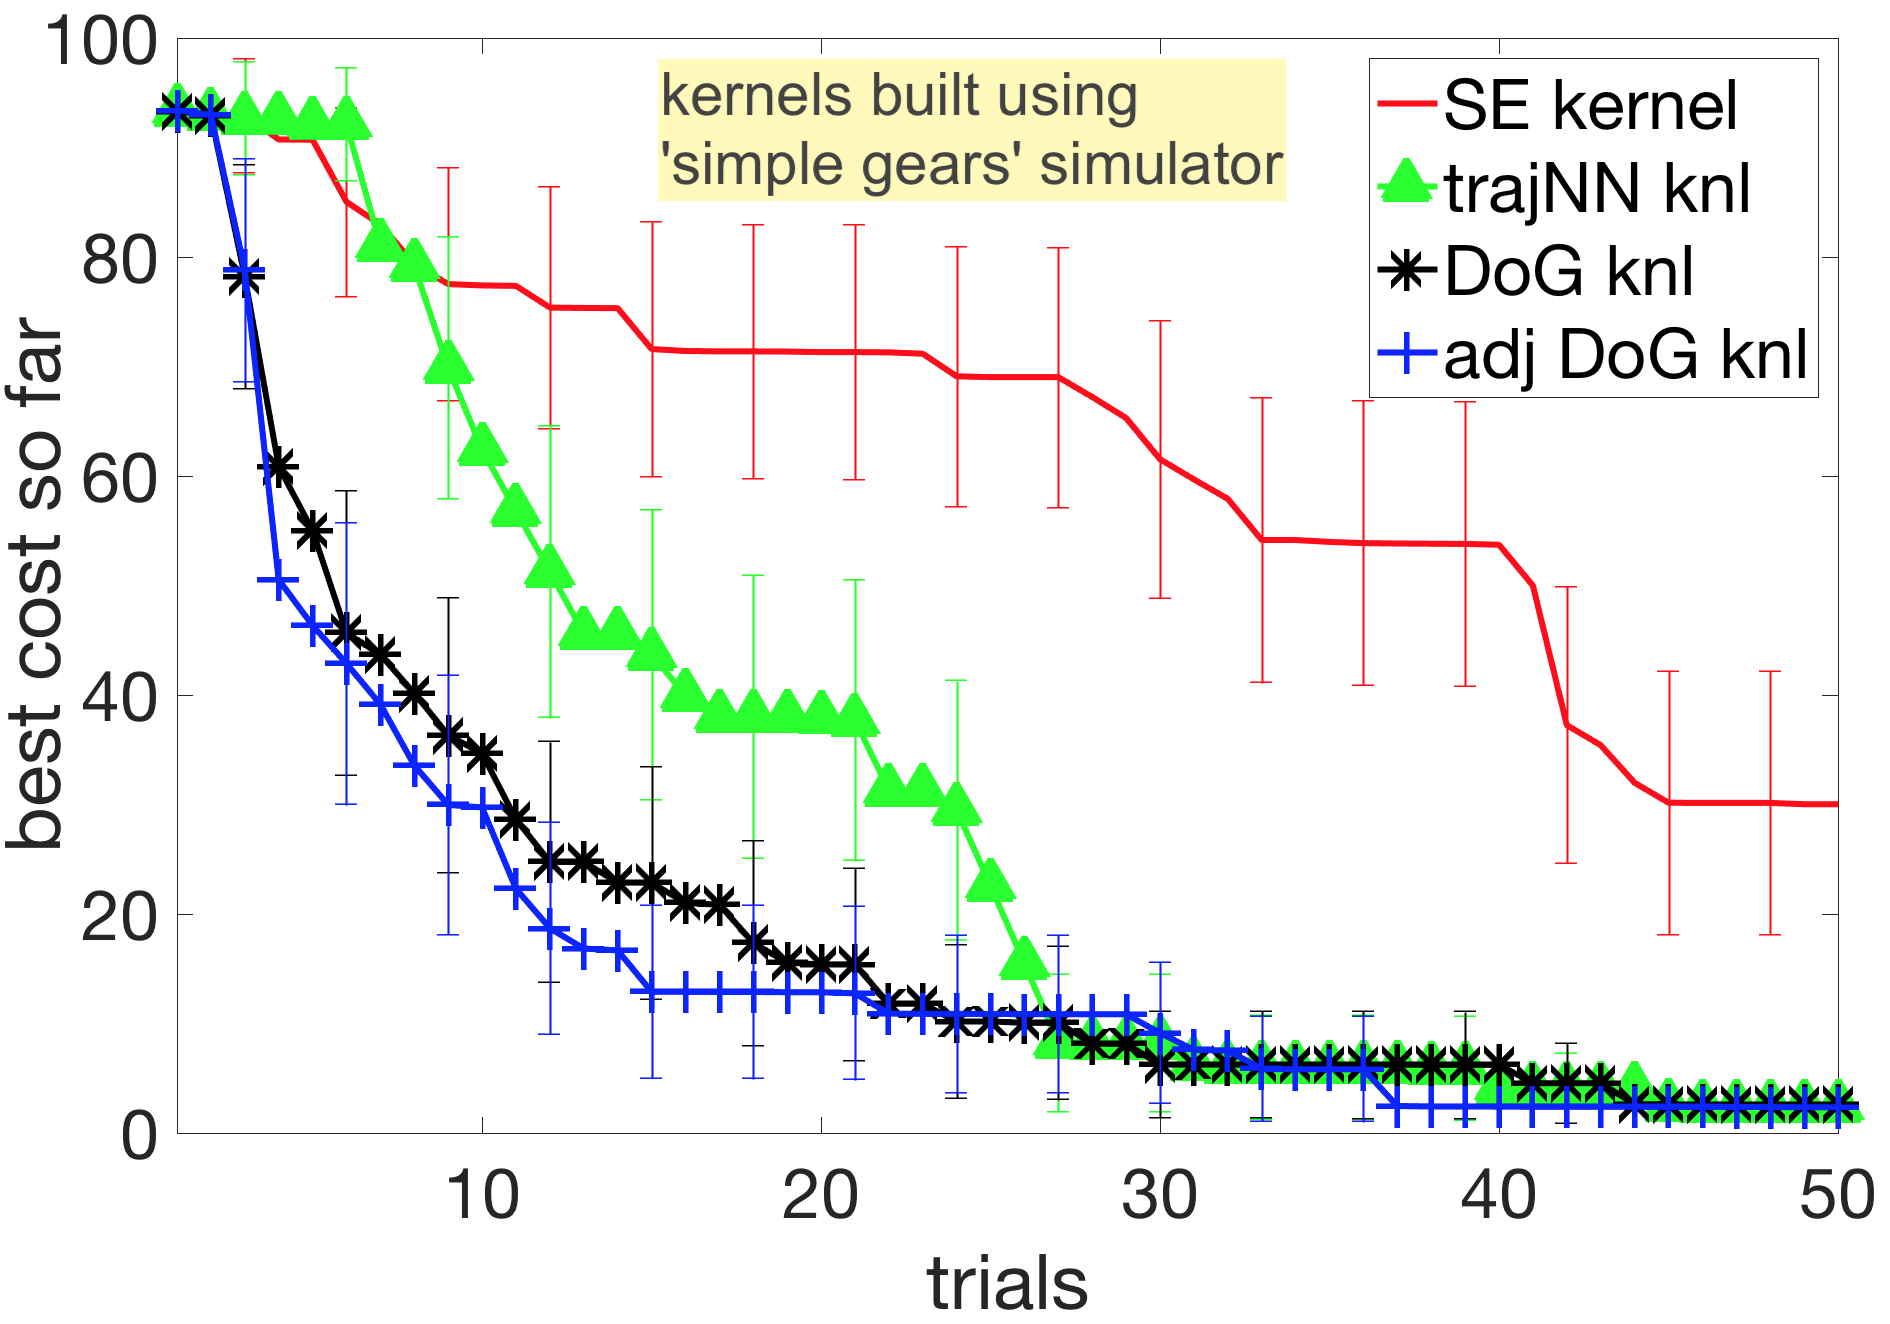
\includegraphics[width=1.0\textwidth]{img/compare_gear_dynamics.png}
\caption{\small{Informed kernels generated using simulator with simplified gear dynamics.}}
\label{fig:compare_gear_dynamics}
\end{subfigure}
\hspace{10px}
\begin{subfigure}[t]{0.47\textwidth}
\centering
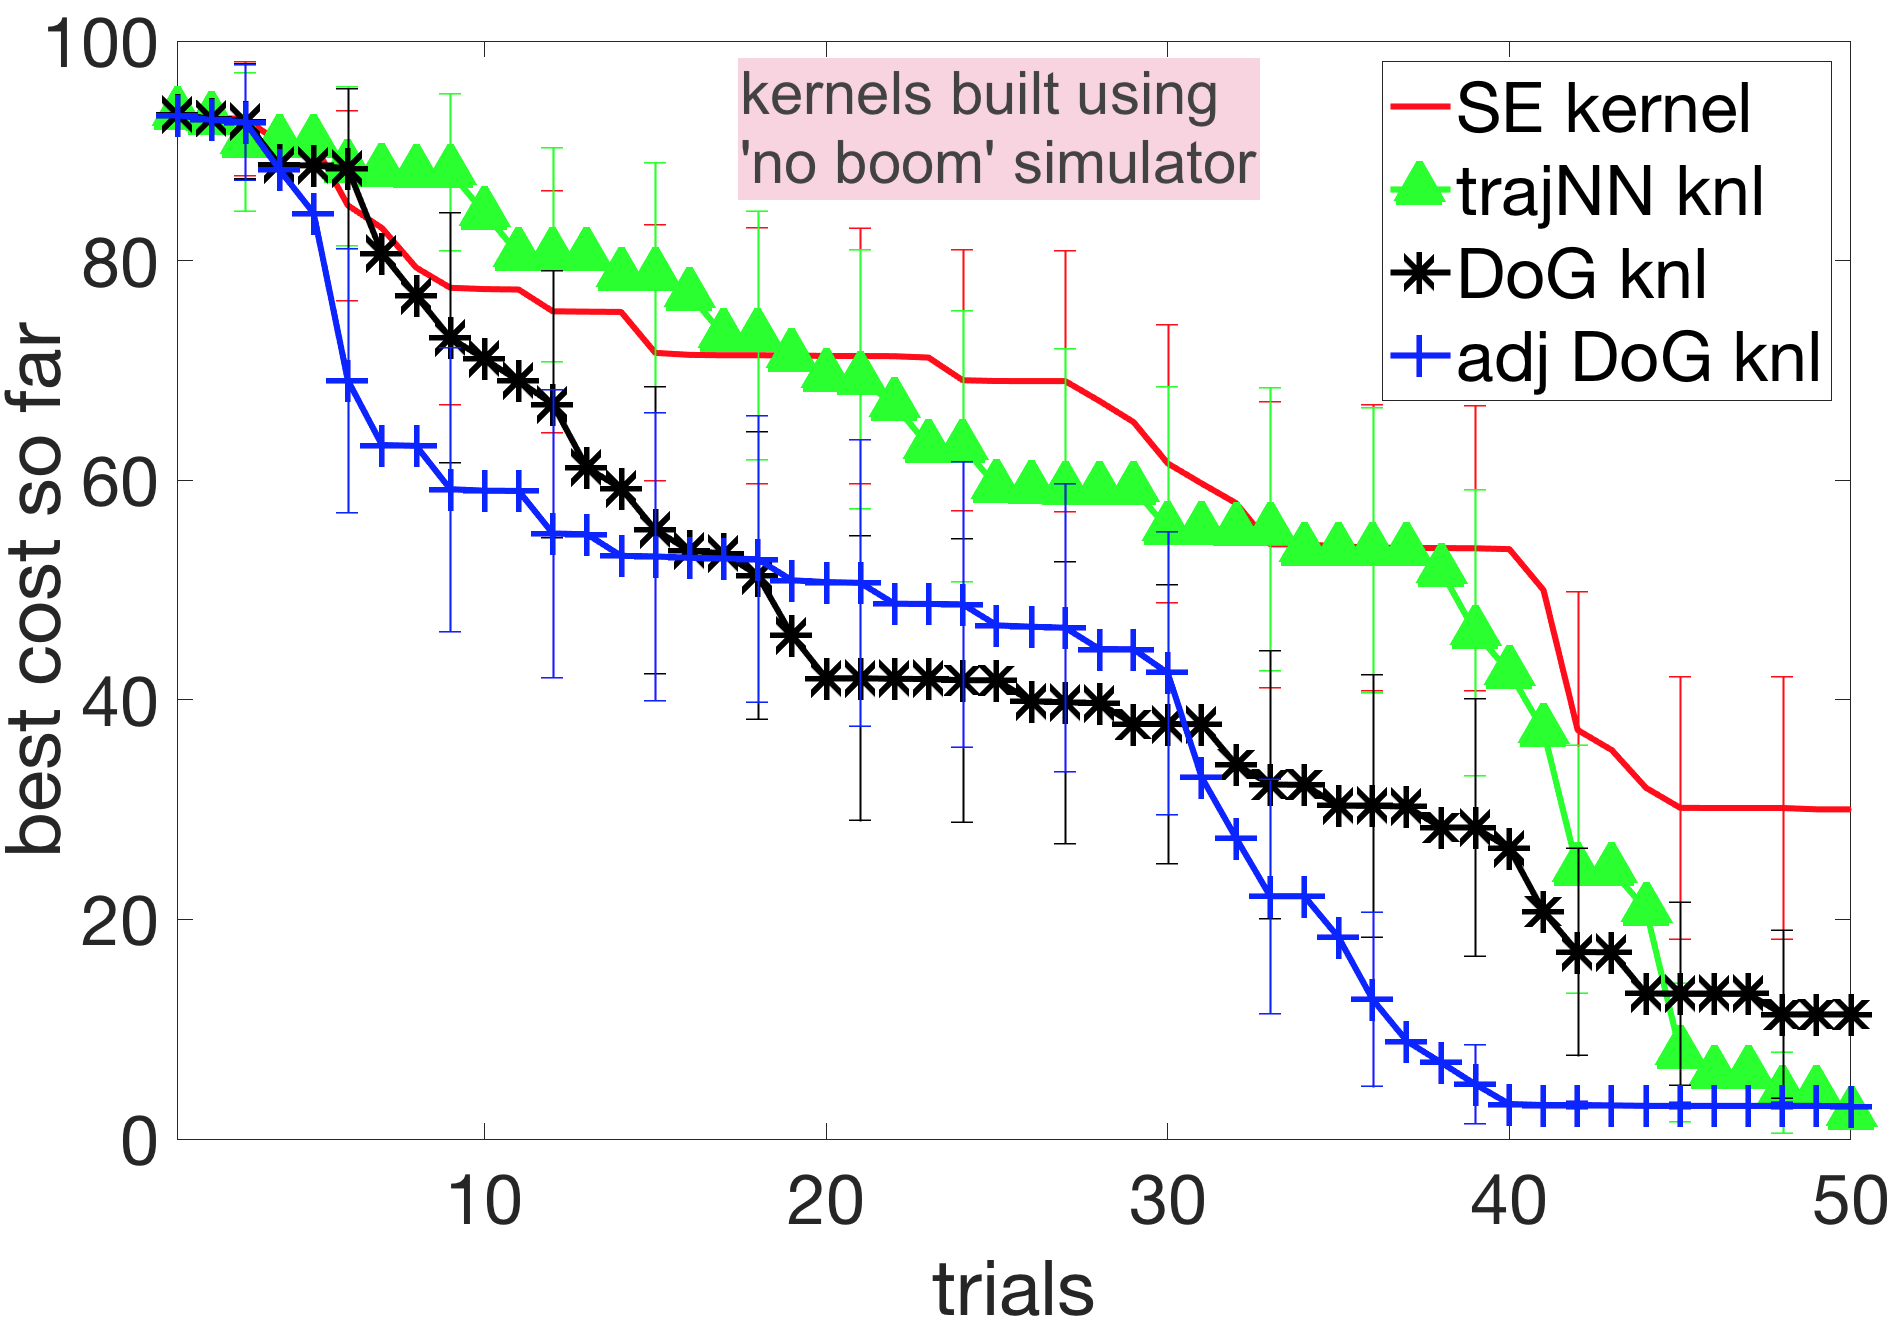
\includegraphics[width=1.0\textwidth]{img/compare_without_boom.png}
\caption{\small{Informed kernels generated using simplified gear dynamics, without boom model.}}
\label{fig:compare_without_boom}
\end{subfigure}
\caption{\small{BO is run on the original simulator. Informed kernels perform well despite significant mismatch, when kernels are generated using simulator with simplified gear dynamics (left). In the case of severe mismatch, when the boom model is also removed, informed kernels still improve over baseline SE (right). Plots show best cost for mean over 50 runs for each algorithm, 95\% CIs.}}
\label{fig:compare_dog}
\end{figure} 
First, we examine the performance of our proposed approaches with informed kernels: $k_{DoG}$, $k_{\text{trajNN}}$ and $k_{DoG_{adj}}$. Figure~\ref{fig:compare_gear_dynamics} shows the case when informed kernels are generated using inaccurate dynamics models, as described in Section \ref{sec:mismatch}. The first approximate simulator has simplified gear dynamics while BO is run on the original simulator. The second approximation removes the boom of the robot and simulates a purely 2-dimensional robot.

When kernel is generated in simulator with approximate gear dynamics, all runs with informed kernels find walking solutions in 50 trials, while for SE only $70\%$ of the runs have walking solutions.

Next, Figure~\ref{fig:compare_without_boom} shows performance of $k_{DoG}$, $k_{\text{trajNN}}$ and $k_{DoG_{adj}}$ when the kernels are constructed using a simulator with simplified dynamics and without a the boom. In this case the mismatch with the original simulator is larger than before and we see the advantage of using adjustment for DoG-based kernel: $k_{DoG_{adj}}$ finds walking points in all runs after 35 trials. $k_{\text{trajNN}}$ also achieves this, but after 50 trials. $k_{DoG}$ finds walking points in $\approx\!90\%$ of the runs after 50 trials. The performance of SE stays the same, as it uses no prior information from any simulator.

This illustrates that while the original DoG-based kernel can recover from slight simulation-hardware mismatch, the adjusted DoG-kernel is required if one expects higher mismatch.  $k_{\text{trajNN}}$ seems to recover from the mismatch, but might benefit from an adjusted version. We leave this to future work.

%------------------------------------------------------------------------------------
\subsubsection{Comparisons of Prior-based and Kernel-based Approaches}
\label{subsec:sim_experiments_prior_cully}
We will classify approaches that use simulation information in hardware optimization as prior-based or kernel-based. Prior-based approaches use costs from the simulation in the prior of the GP used in the BO. This can help BO a lot if the costs between simulation and hardware transfer, and the cost function is fixed. However, in the presence of large mismatch, points that perform well in simulation might fail on hardware. A prior-based method can be biased towards sampling promising points from simulation, resulting in an even poorer performance than methods with no prior. Kernel-based approaches consist of methods that incorporate the information from simulation into the kernel of the GP. These can be sample-inefficient as compared to prior-based method, but less likely to be biased towards unpromising regions in the presence of mismatch. They also easily generalize to multiple costs, so that there is no additional computation if the cost is changed. This is important because a lot of these approaches can take several days of computation to generate the informed kernel. For example, \cite{cully2015robots} report taking 2 weeks on a 16-core computer to generate their map. 
\begin{figure}[t]
\begin{subfigure}[t]{0.47\textwidth}
\centering
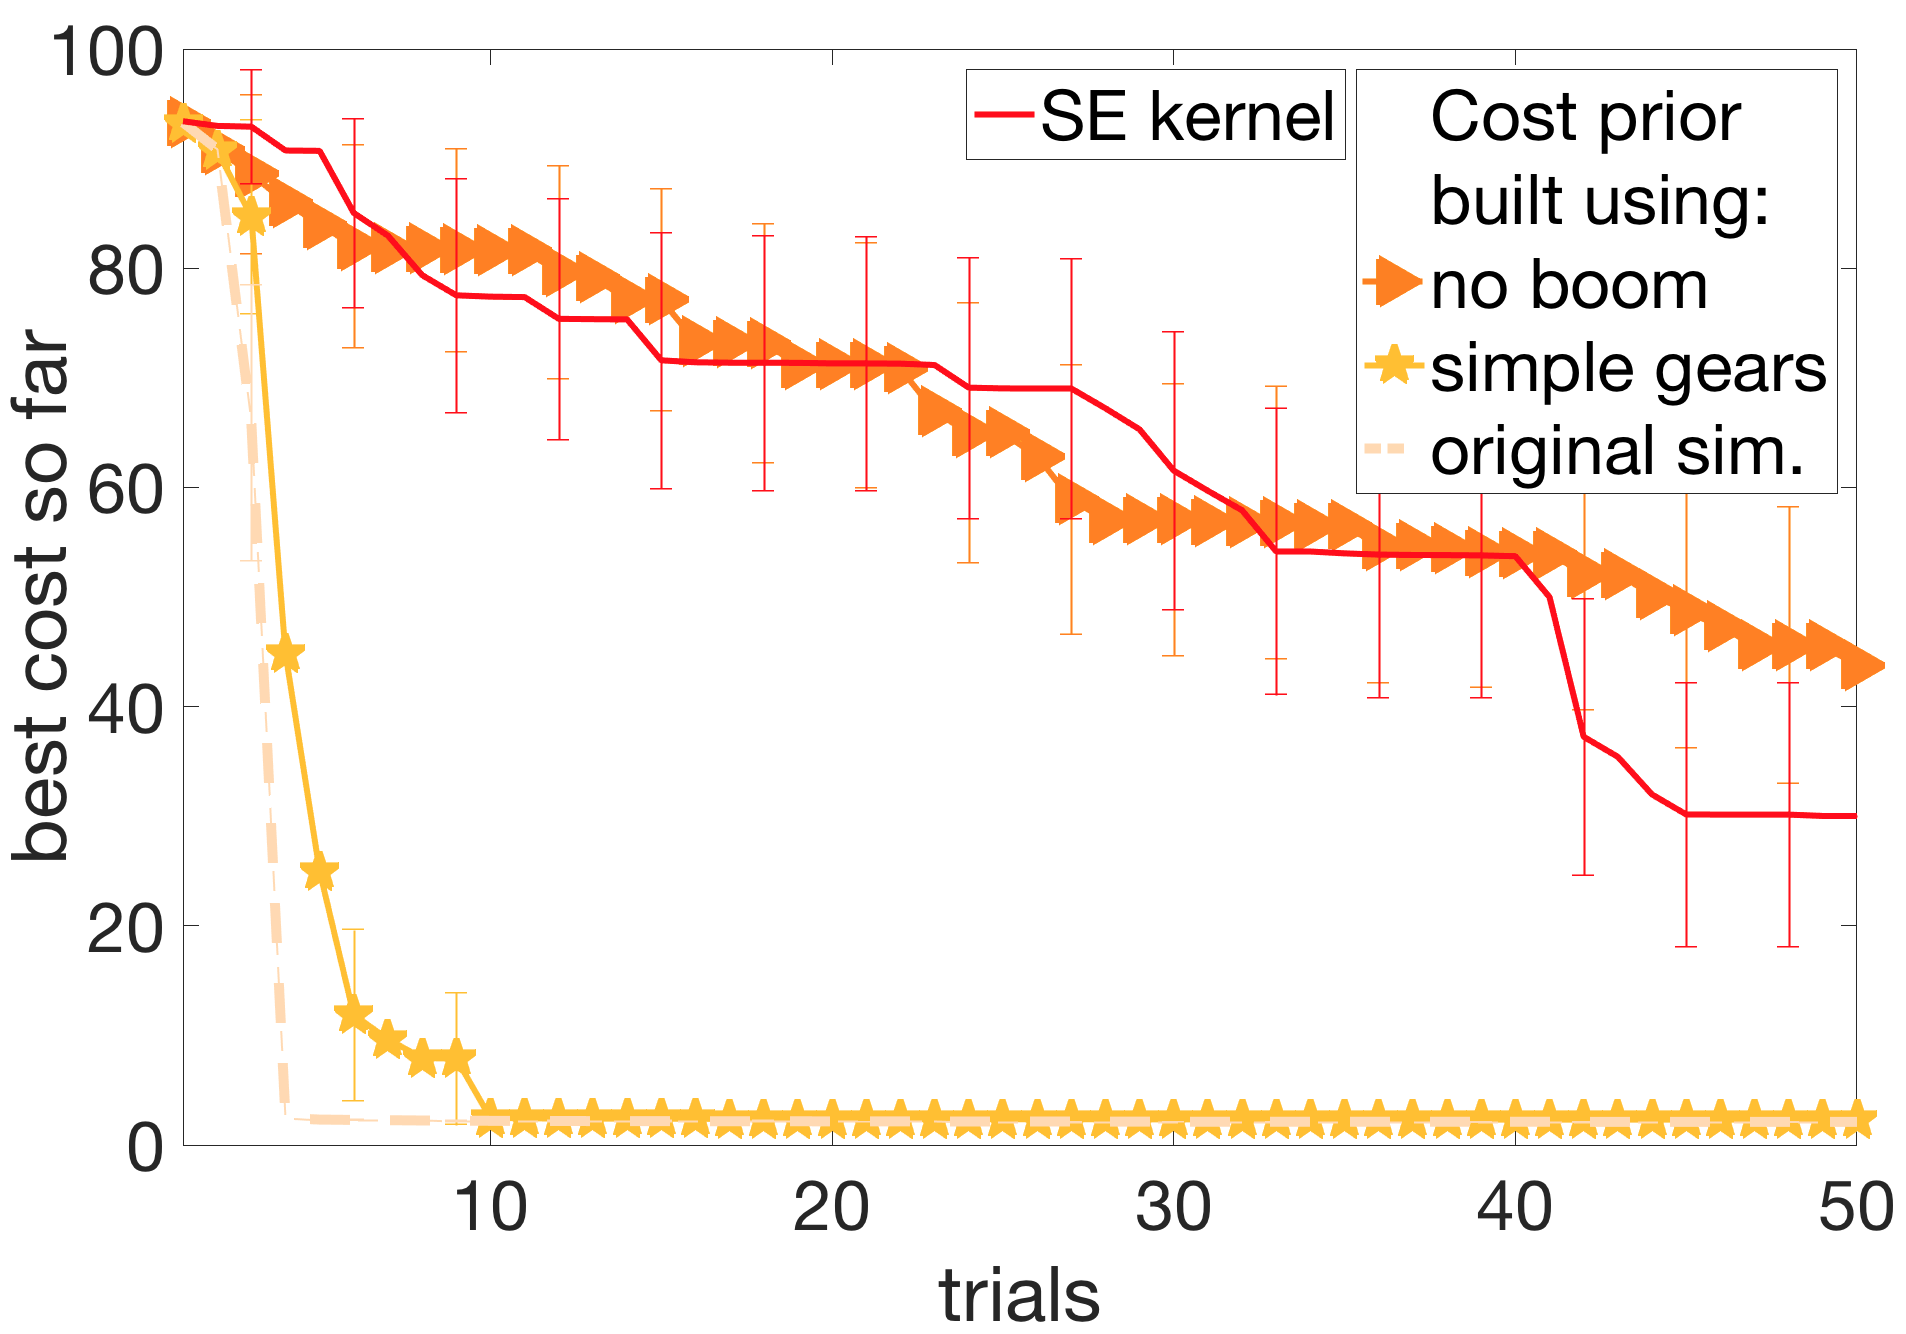
\includegraphics[width=1.0\textwidth]{img/cost_prior_sim_versions.png}
\caption{\small{BO with cost prior: straightforward approach useful for low-to-medium mismatch; but no improvement if mismatch is severe.}}
\label{fig:cost_prior_sim_versions}
\end{subfigure}
\hspace{15px}
\begin{subfigure}[t]{0.47\textwidth}
\centering
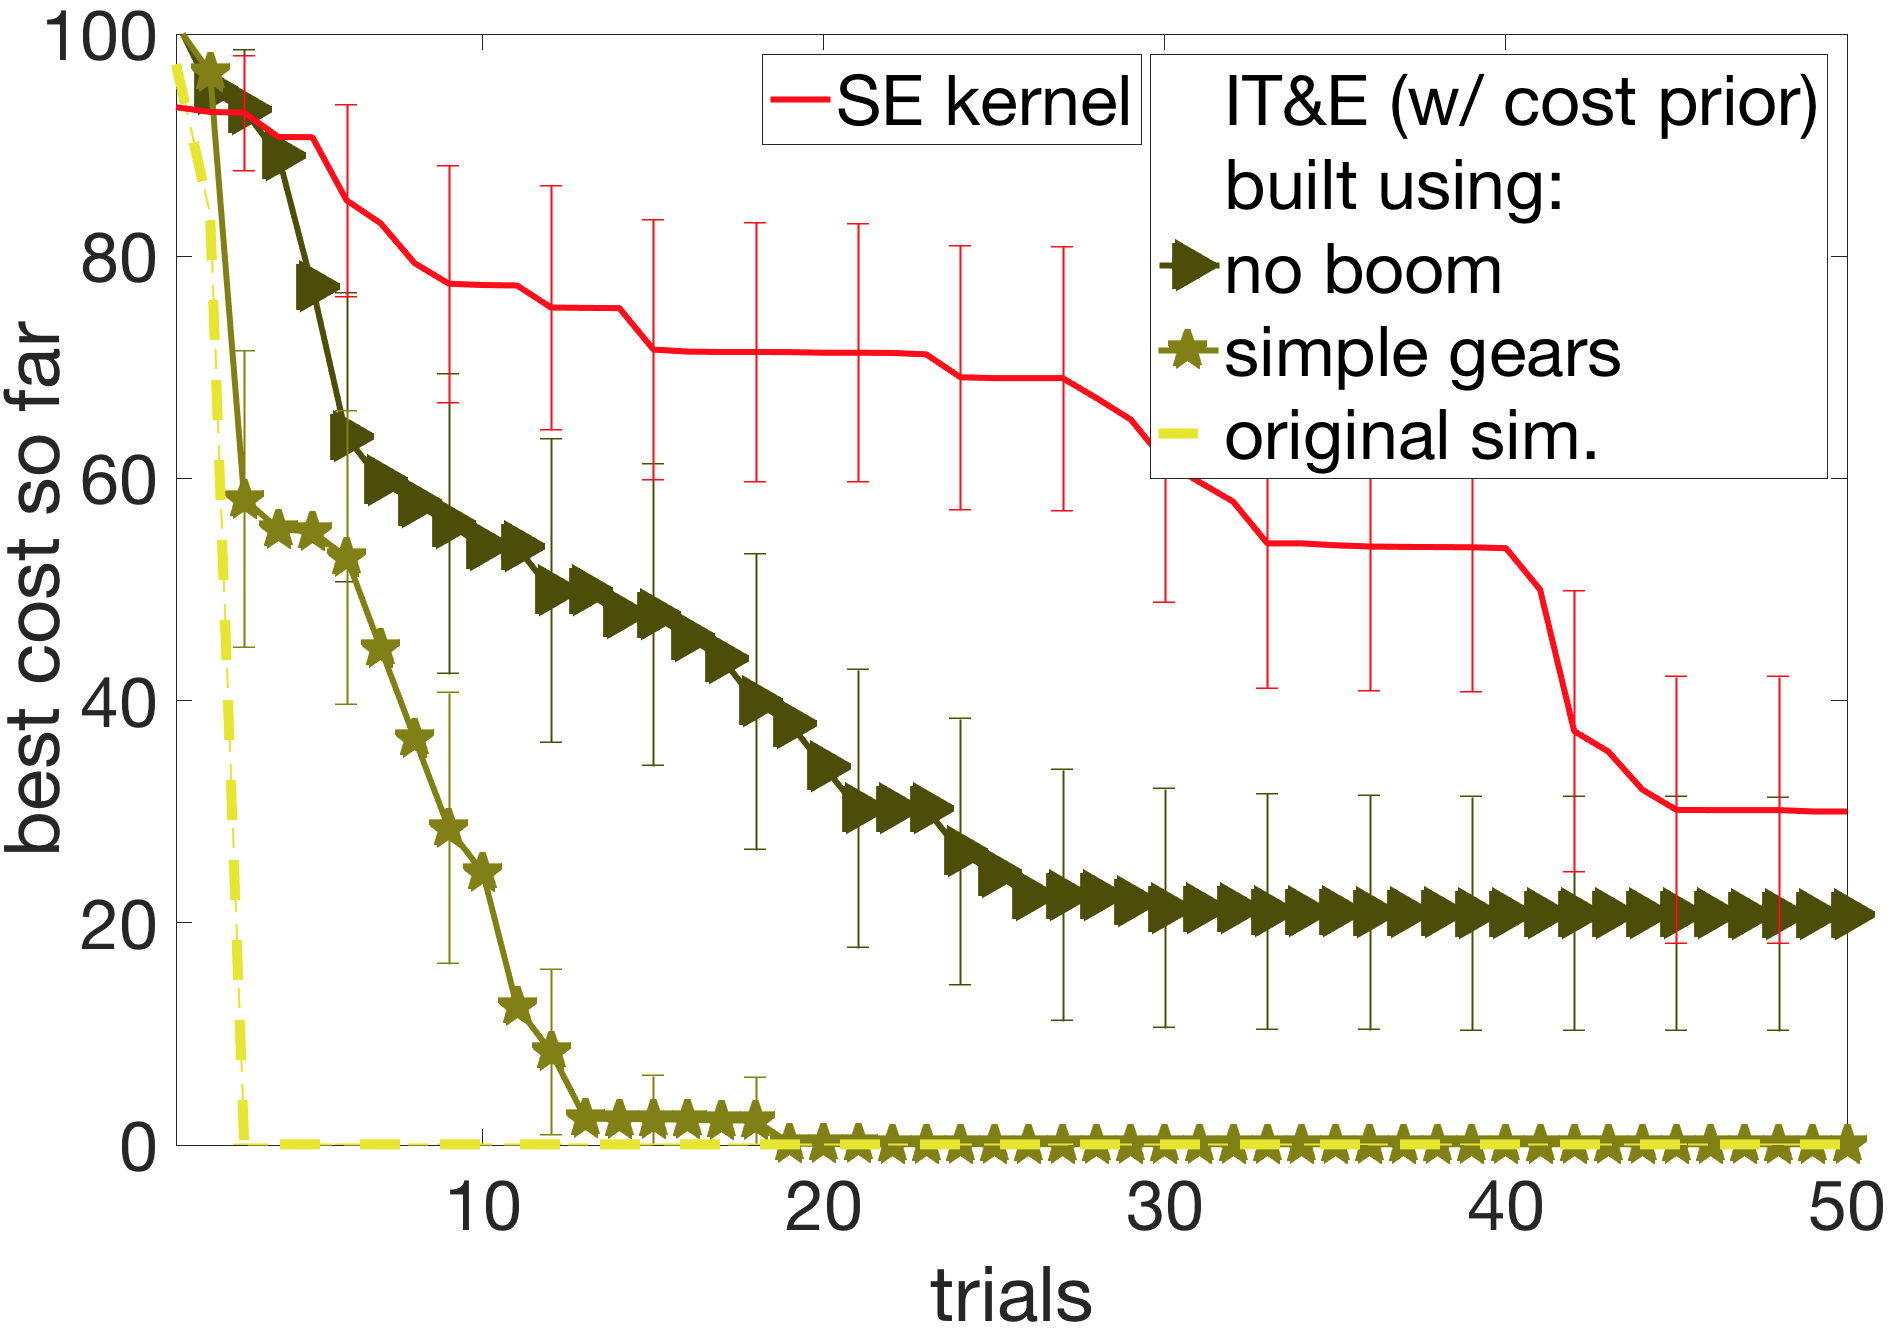
\includegraphics[width=1.0\textwidth]{img/cully_prior_sim_versions.png}
\caption{\small{Performance of IT\&E algorithm (our implementation of \citet{cully2015robots}, adapted to bipedal locomotion).}}
\label{fig:cully_prior_sim_versions}
\end{subfigure}
\caption{\small{BO using prior-based approaches. Mean over 50 runs for each algorithm, 95\% CIs.}}
\label{fig:prior_based_bo}
\end{figure}

It is possible to also combine both prior-based and kernel-based methods, as in \cite{cully2015robots}. We will classify these as `prior-based' methods, since in our experiments prior outweighs the kernel effects for such cases. In our comparison with \cite{cully2015robots}, we will implement a version with and without the prior points. We do not add a cost prior to BO using DoG-based kernel, as this limits us to a particular cost, and high-fidelity simulators. Since both of these can be major obstacles in real robot experiments, we refrain from doing so.


Figure~\ref{fig:cost_prior_sim_versions} shows the performance when using simulation cost in the prior during BO, and learning a model for the difference between simulation and hardware costs \citep{wilson2014using}. BO with a cost prior created using the original version of the simulator illustrates what would happen in the best case scenario, as optimization is merely a look-up here. When the simulator with simplified gear dynamics is used for constructing the prior, we observe significant improvements over uninformed BO prior. However, when the prior is constructed from simplified gear dynamics and no boom setting, the approach performs slightly worse than uninformed BO. This shows that while an informed prior can be very helpful when created from a simulator close to hardware, it can hurt performance if simulator is significantly different from hardware. 


\begin{figure}[t]
\begin{subfigure}[t]{0.47\textwidth}
\centering
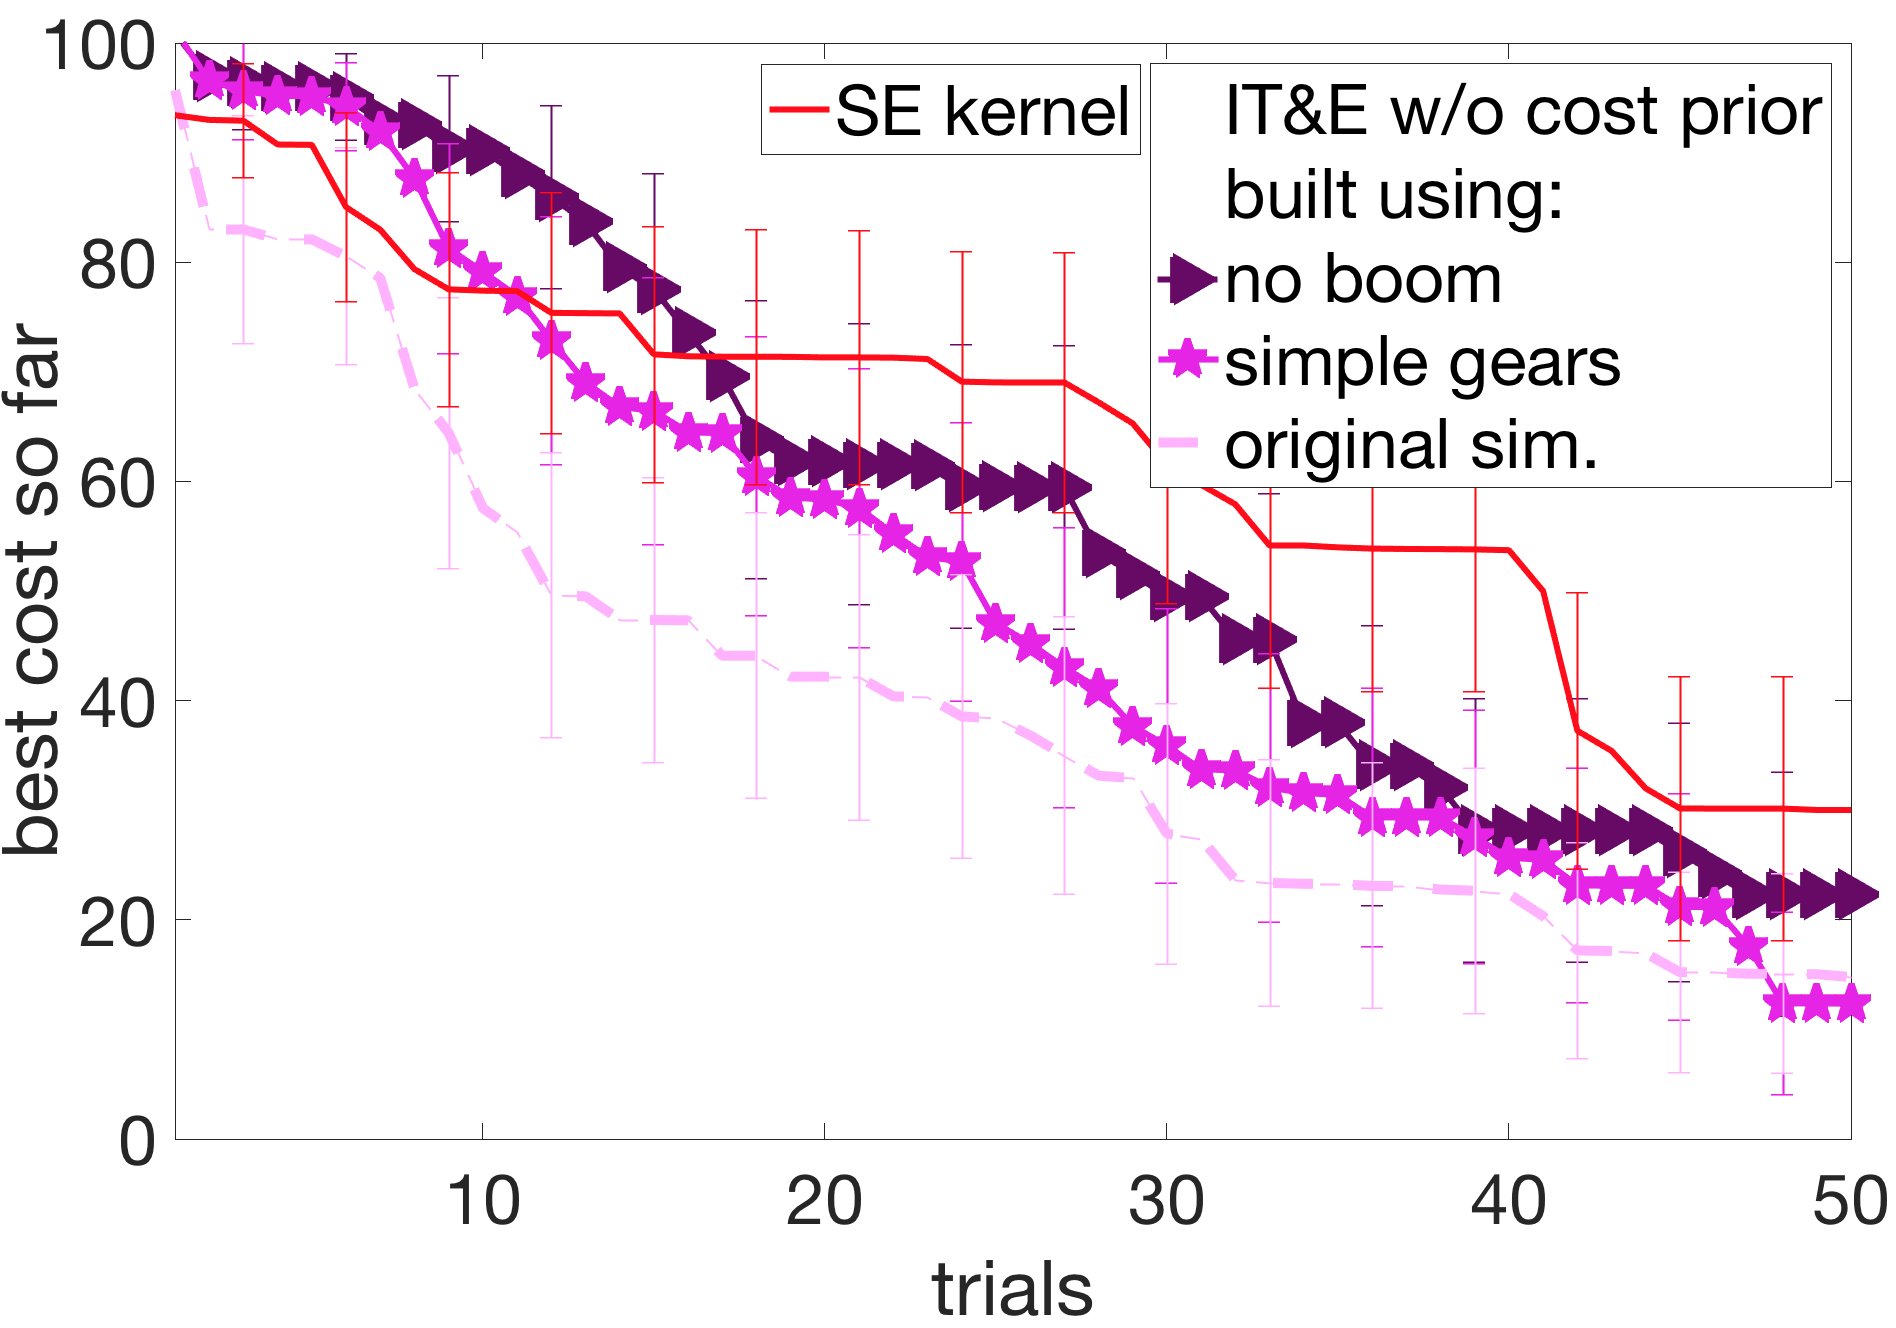
\includegraphics[width=1.0\textwidth]{img/cully_no_prior_sim_versions.png}
\caption{\small{BO using our implementation of IT\&E without cost prior (from \citet{cully2015robots}).}}
\label{fig:cully_kernel_sim_versions}
\end{subfigure}
\hspace{10px}
\begin{subfigure}[t]{0.47\textwidth}
\centering
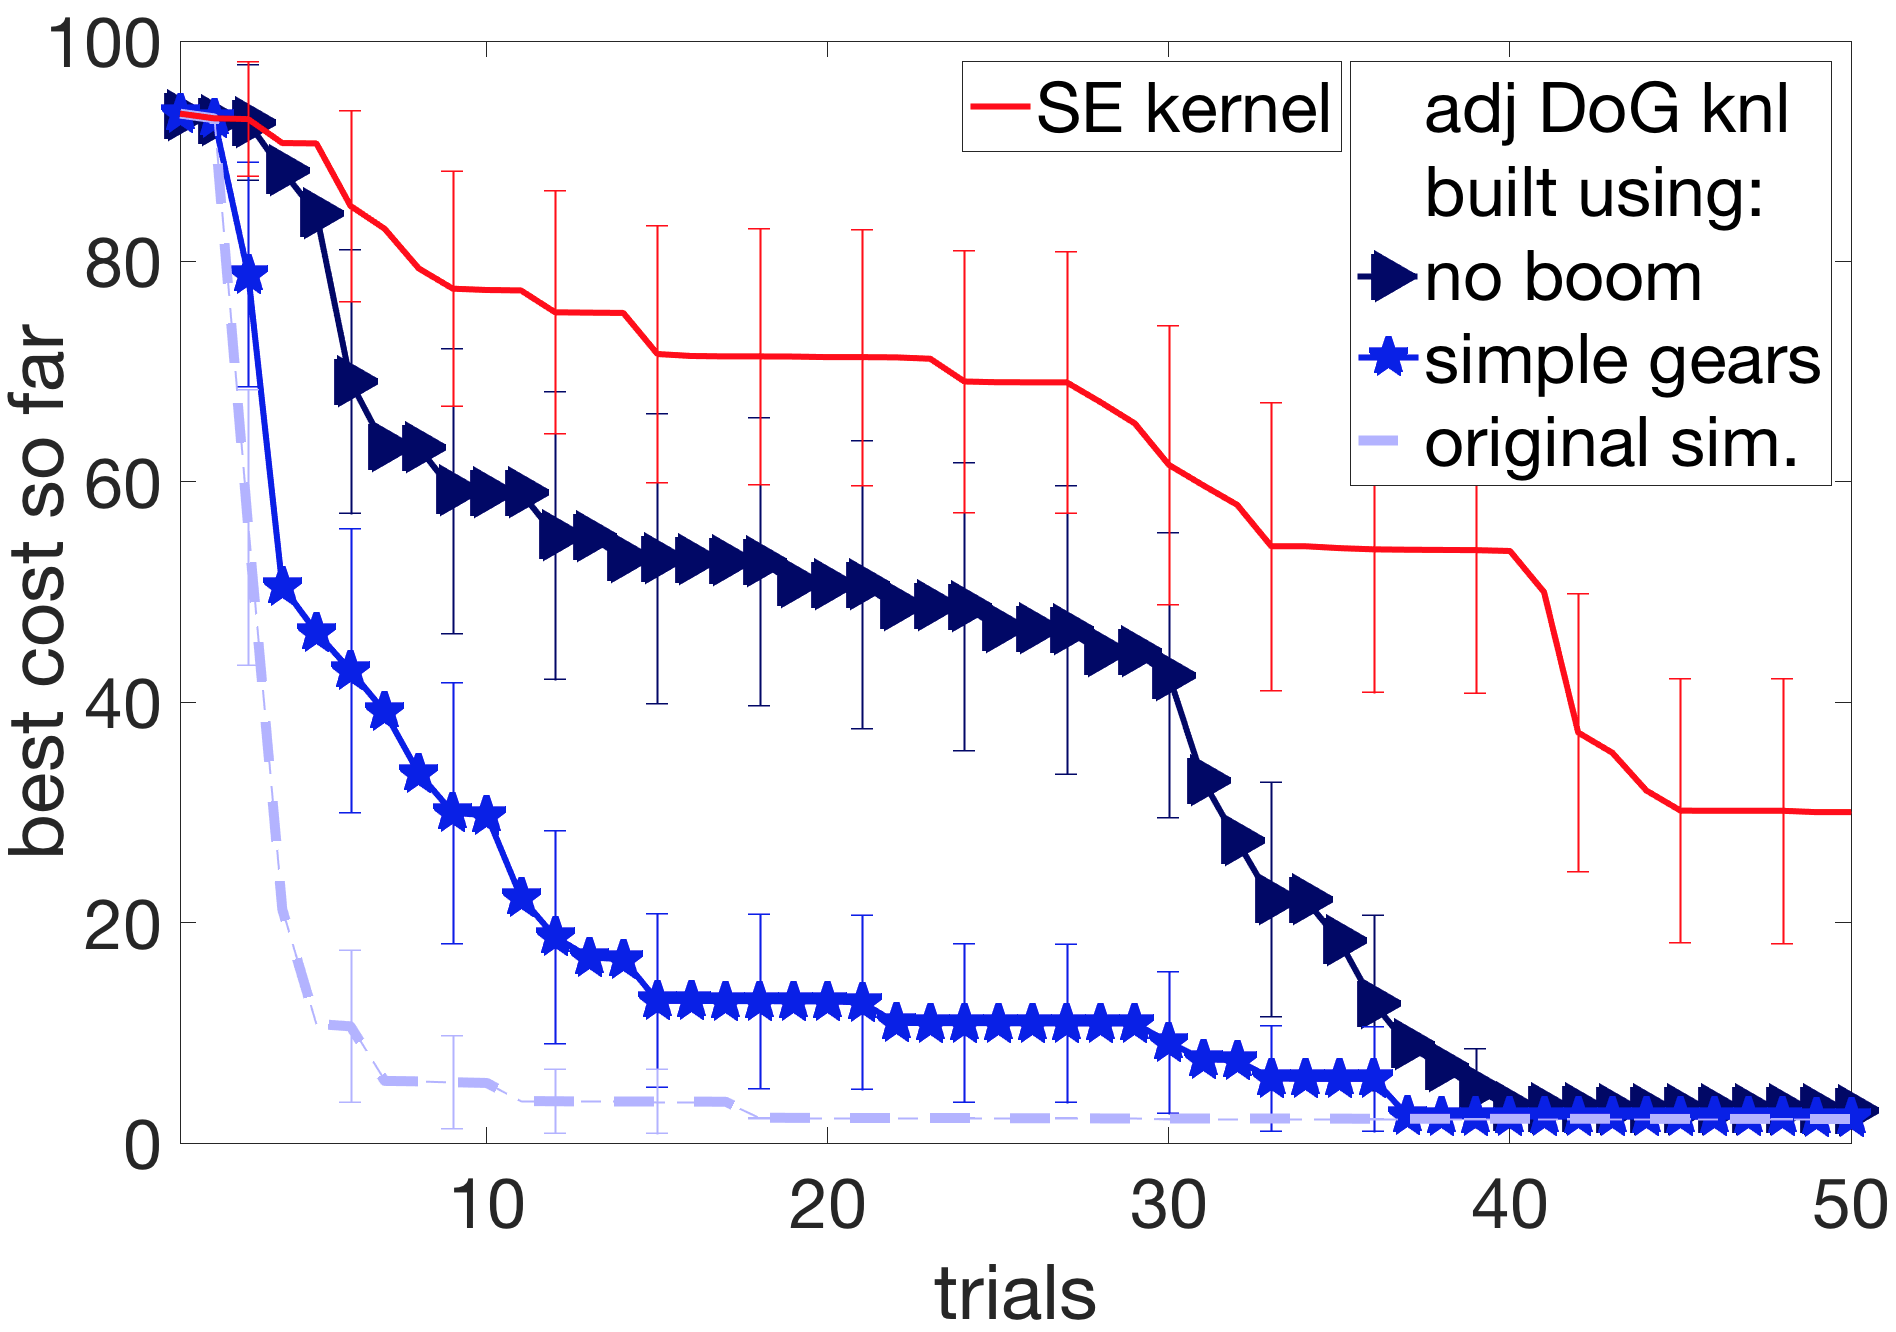
\includegraphics[width=1.0\textwidth]{img/dog_hwadjust1_sim_versions.png}
\caption{\small{BO using $k_{DoG_{adj}}$ constructed from simulators with various levels of mismatch.}}
\label{fig:kernel_hwadjust2_sim_versions}
\end{subfigure}
\caption{\small{BO using kernel-based approaches. Mean over 50 runs for each algorithm, 95\% CIs.}}
\label{fig:prior_based_bo}
\end{figure}


Next, we discuss experiments with our implementation of Intelligent Trial and Error (IT\&E) algorithm from~\citet{cully2015robots}. This algorithm combines adding a cost prior from simulated evaluations with adding simulation information into the kernel. IT\&E defines a behavior metric and tabulates best performing points from simulation on their corresponding behavior score. The behavior metric used in our experiments is duty-factor of each leg, which can go from 0 to 1.0. We discretize the duty factor into 21 cells of 0.05 increments, leading to a $21\times21$ grid. We collect the 5 highest performing controllers for each square in the behavior grid, creating a $21\times21\times5$ grid. Next, we generate 50 random combinations of a $21\times21$ grid, selecting 1 out of the 5 best controllers per grid cell. Care was taken to ensure that all 5 controllers had comparable costs in the simulator used for creating the map. 
Cost of each selected controller is added to the prior and BO was performed in the behavior space, like in \cite{cully2015robots}.

Figure~\ref{fig:cully_prior_sim_versions} shows BO with IT\&E constructed using different versions of the simulator. \mbox{IT\&E} constructed using simplified gear dynamics simulator is slightly less sample-efficient than the straightforward `cost prior' approach. When constructed with the simulator with no boom, \mbox{IT\&E} is able to improve over uninformed BO. However, it only finds walking points in 77\% of the runs in 50 trials in  this case, as some of the generated maps contained no controllers that could walk on the `hardware'. This is a shortcoming of the IT\&E algorithm, as it eliminates a very large part of the search space and if the pre-selected space does not contain a walking point, no walking controllers can be sampled with BO. This problem could possibly be avoided by using a finer grid, or a different behavior metric. However tuning such hyper-parameters can turn out to be expensive, in computation and hardware experiment time.
 


To separate the effects of using simulation information in prior mean vs kernel, we evaluated a kernel-only version of \mbox{IT\&E} algorithm. Figure~\ref{fig:cully_kernel_sim_versions} shows these results. It shows that the cost prior is crucial for the success of IT\&E and performance deteriorates without it. Hence, it is not practical to use IT\&E on a cost different than what it was generated for.

Nonetheless, Figure~\ref{fig:compare_dog} showed that BO with adjusted DoG kernel is able to handle both moderate and severe mismatch with kernel-only information, collected in  Figure~\ref{fig:kernel_hwadjust2_sim_versions}.

In summary, we created two simulators with increasing modelling approximations, and studied the effect of using these to aid optimization on the original simulator. We found that while methods that use cost in the prior of BO can be very sample-efficient in low mismatch, their performance worsens as mismatch increases. \mbox{IT\&E} introduced in \cite{cully2015robots} uses simulation information in both prior mean and kernel, and is very sample-efficient in cases of low mismatch. Even with high mismatch, it performs better than just prior-based BO but doesn't find walking controllers reliably. In comparison, adjusted DoG-based kernel performed well in all the tested scenarios. All of this shows that the adjusted DoG-based kernel can reliably improve sample-efficiency of BO even when the mismatch between simulation and hardware is high. We would like to continue working in this direction and explore the usefulness of even simpler simulators in the future.

%\AR{Add note about smooth cost and performance}

\subsection{Incorrect dynamics parameters}

Our next set of experiments create ``simulated hardware" that is increasingly different from the simulation, in which the DoG features were collected. This is done by changing the mass, inertia, center of mass location, friction coefficient of the ground contact models, ground stiffness and actuator delay, as described in Section \ref{sec:mismatch}.

\begin{figure}[h!]
\centering
    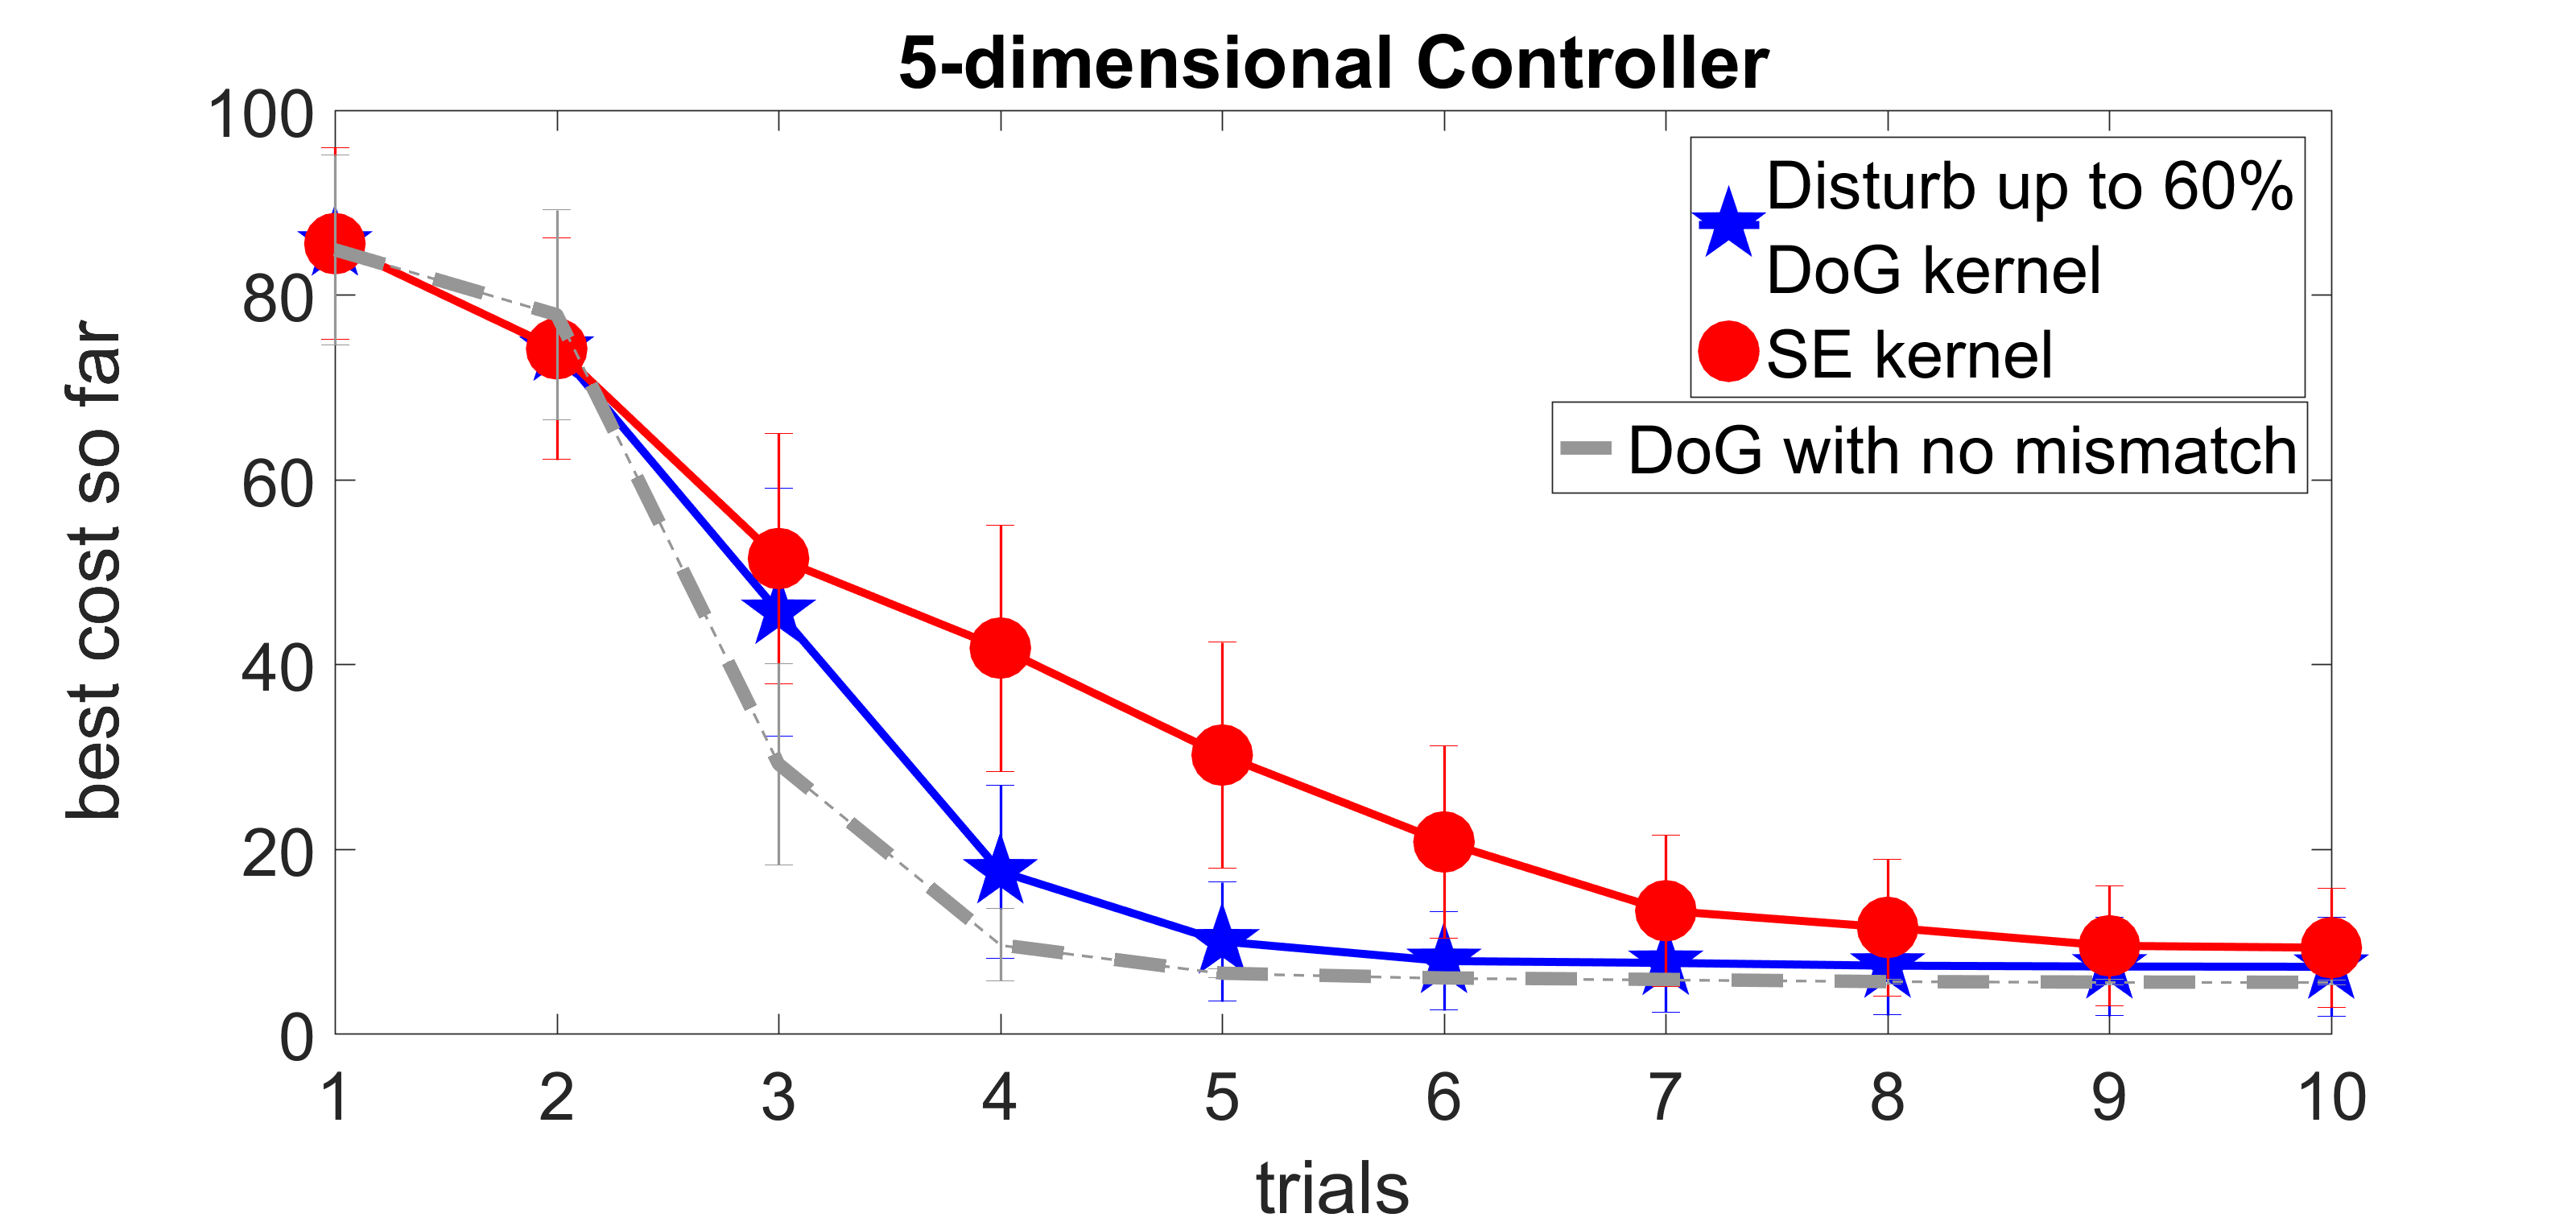
\includegraphics[width=0.65\textwidth]{img/BO_kernel_5d_disturb.png}
    \vspace{0.15cm}
    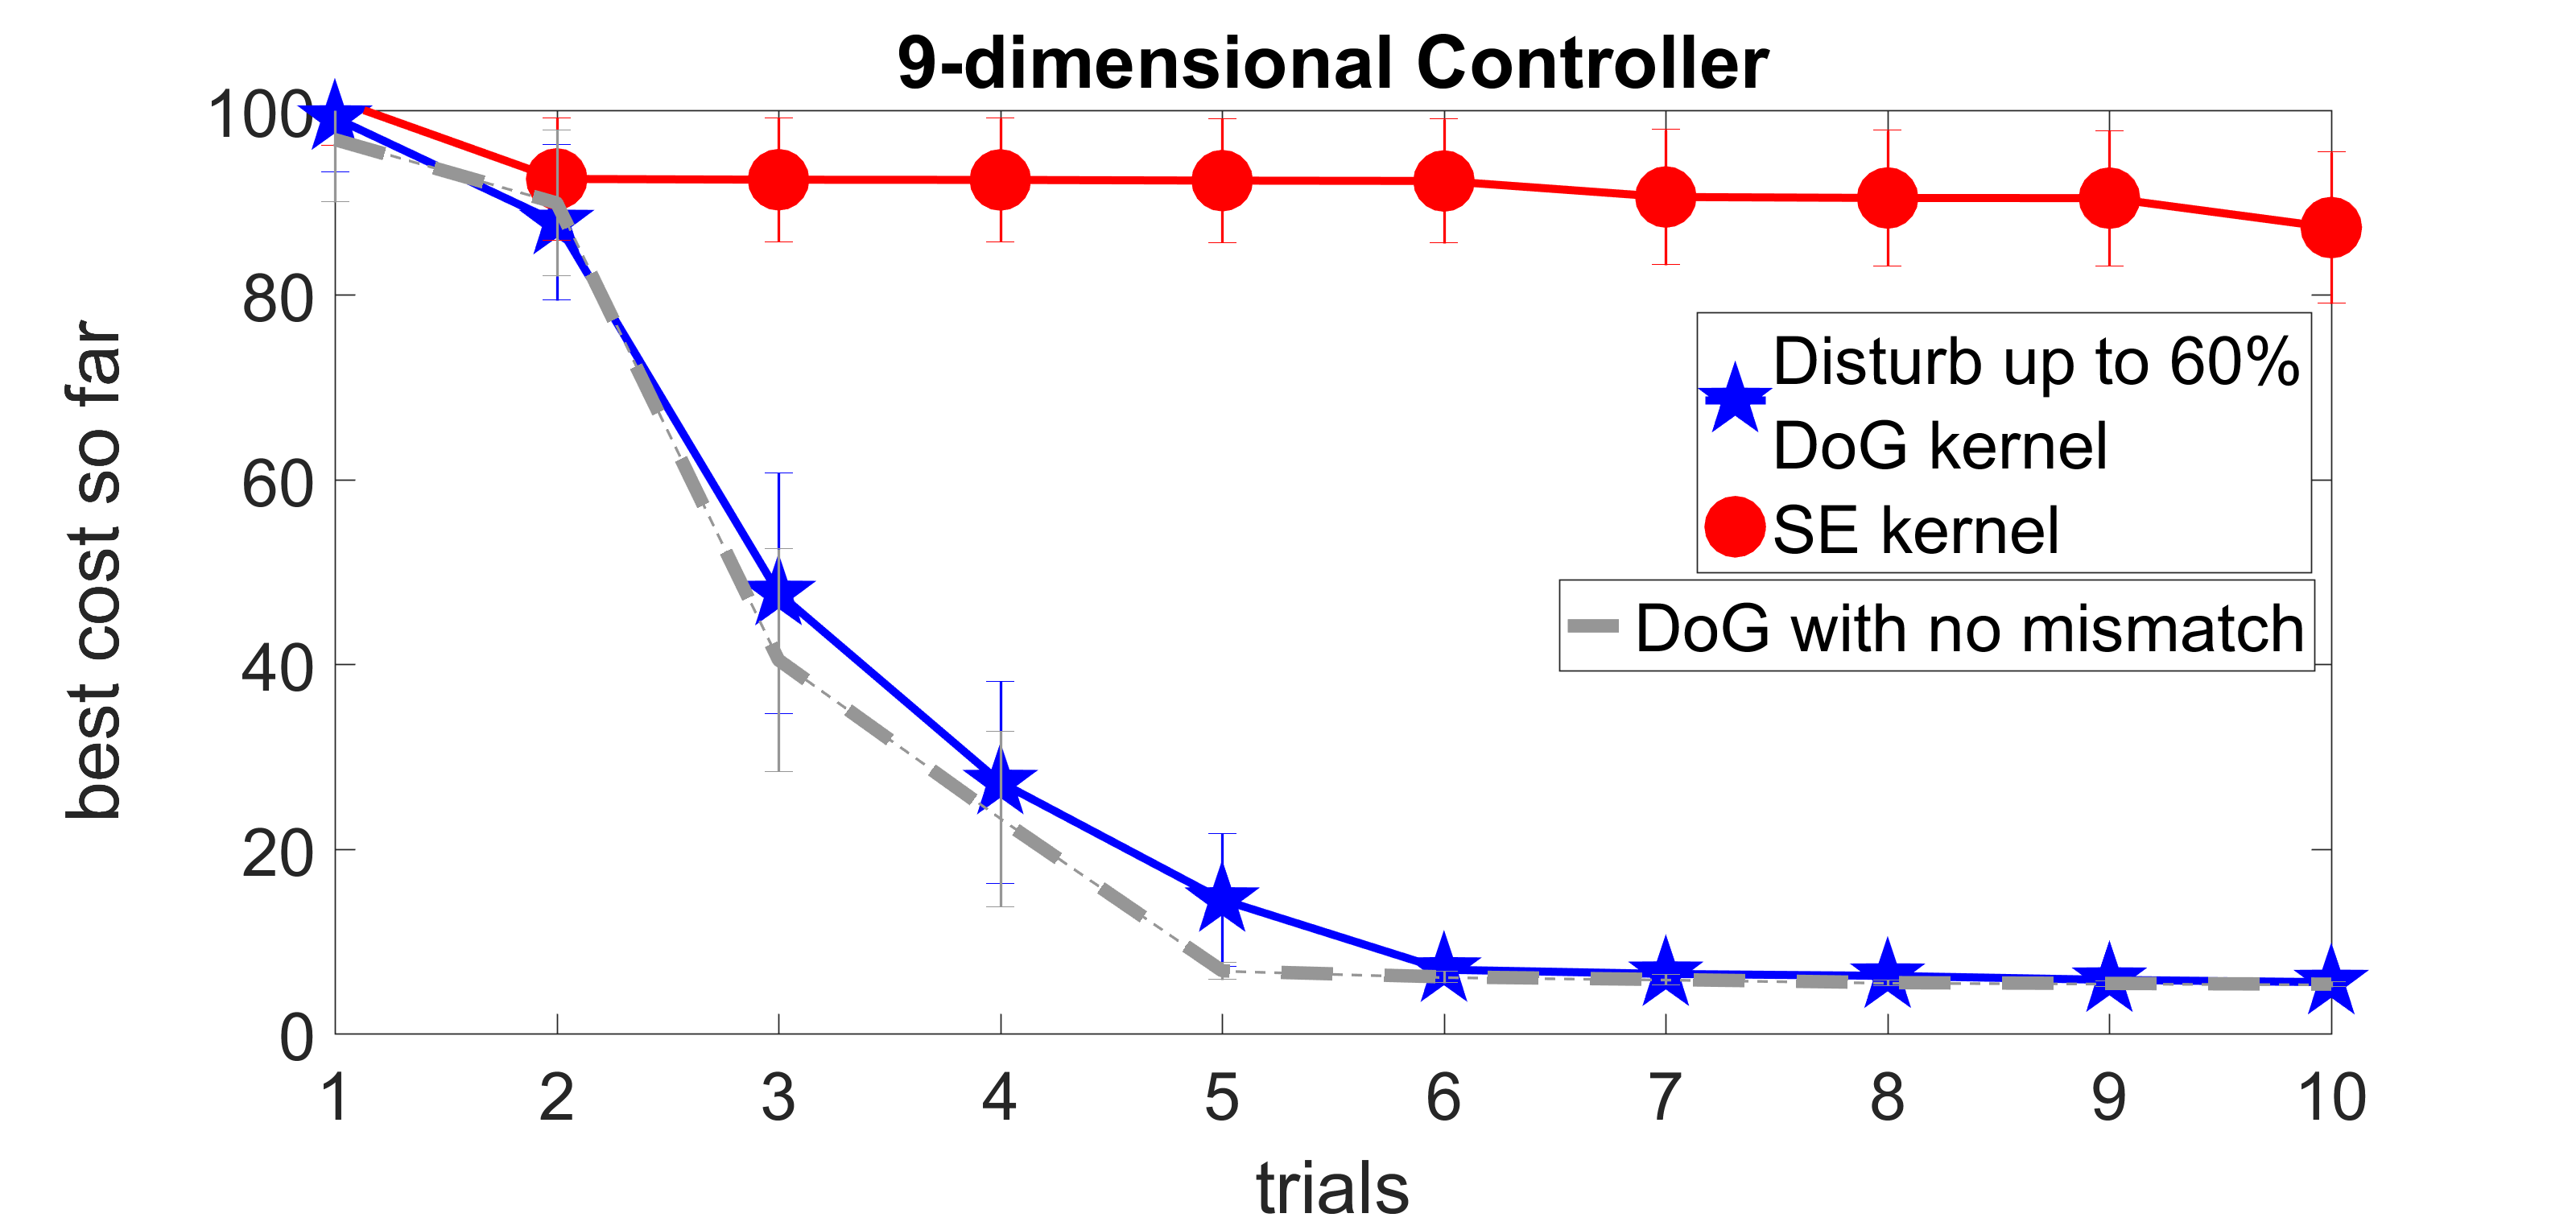
\includegraphics[width=0.65\textwidth]{img/BO_kernel_9d_disturb.png}
    \vspace{0.15cm}
    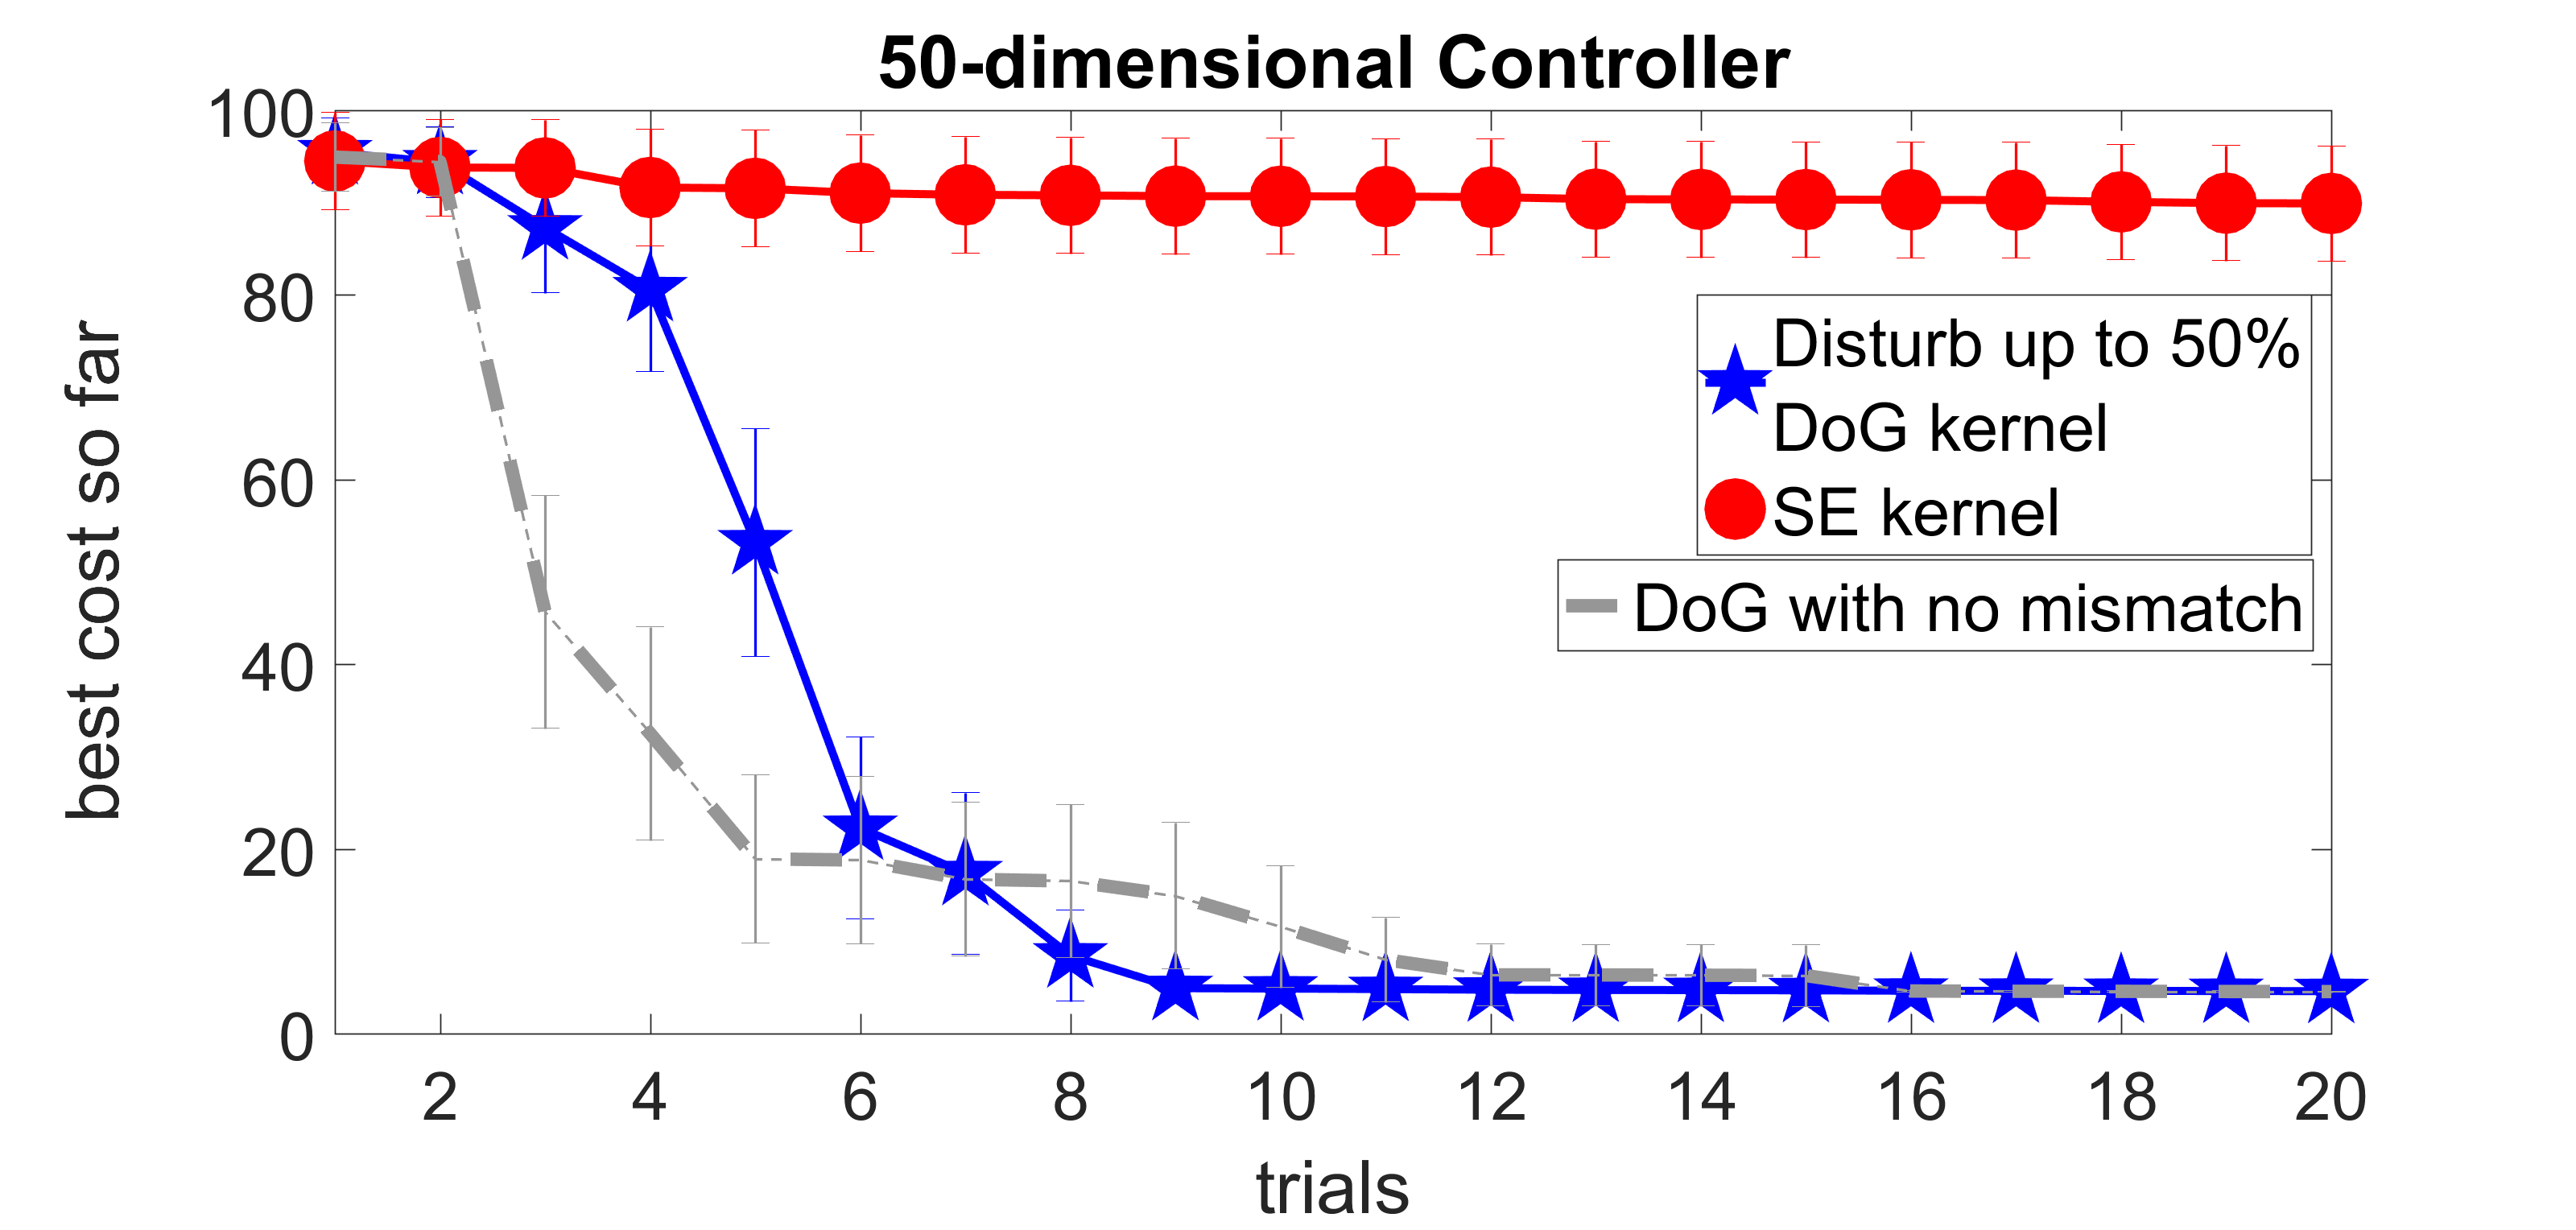
\includegraphics[width=0.65\textwidth]{img/BO_kernel_50d_disturb.png}
    \caption{Performance of DoG and SE kernel with disturbance for 5-dimensional (top), 9-dimensional (middle) and 50-dimensional (bottom) controllers over 50 runs. DoG with no simulation-hardware mismatch is also shown. DoG performs better than SE even on maximum disturbance, and performance does not deteriorate as disturbance increases.}
    \label{fig:dist_controllers}
\end{figure}

As shown in Figure \ref{fig:dist_controllers}, adjusted-DoG kernel obtains walking controllers in less than 10 trials for 5 and 9-dimensional controllers with up to $\pm$ 60\% perturbation of dynamics parameters. In comparison, while for the 5-dimensional controller BO with SE finds walking controllers in less than 10 trials, its performance deteriorates for the 9-dimensional controller. 
Our approach can scale well even to 50 dimensions, learning walking VNMC controllers reliably in less than 20 trials, with up to $\pm$ 50\% perturbation of dynamics parameters.


